\documentclass[a4paper,11pt,oneside,brazilian,
draft=false]{report}%openany,version=last

\setlength{\columnsep}{15pt}
\usepackage{float} 
\usepackage{rotating}
\usepackage{graphicx}
\usepackage{mybook}
\usepackage{fancyhdr} 
\usepackage{pdflscape}
\usepackage{pdfpages} 
\usepackage[toc,page]{appendix}
\usepackage{titlesec}
\usepackage{xcolor}
\usepackage{framed}
\usepackage{titletoc}
\usepackage{longtable}
\usepackage[brazilian]{babel} 
\usepackage{hyperref} 
\usepackage[position=b]{subcaption}
\usepackage{wrapfig}
\usepackage{natbib}        % required for bibliography


\newcommand*{\fancychapterstyle}{%
  \titleformat{\chapter} % command
	[block] % shape
	{\bfseries\Large\itshape} % format
	{	\textsc{\LARGE Relatório Final do Projeto EMMA} 
		\newline \newline  
		\textsc{\Large Capítulo \ \thechapter}
	} % label
	{0.5ex} % sep
	{
    	\rule{\textwidth}{2pt}
    	\vspace{1ex}
    	\centering
    	\huge \textnormal
	} % before-code
	[
		\vspace{-1ex}%
		\rule{\textwidth}{2pt}
		\vfill 
\includegraphics{logo/EMMA-logo}
	] % after-code
}

\newcommand*{\fancyappendixstyle}{%
  \titleformat{\chapter} % command
	[block] % shape
	{\bfseries\Large\itshape} % format
	{	\textsc{\LARGE Relatório Final do Projeto EMMA} 
		\newline \newline  
		\textsc{\Large Apêndice \ \thechapter}
	} % label
	{0.5ex} % sep
	{
    	\rule{\textwidth}{2pt}
    	\vspace{1ex}
    	\centering
    	\huge \textnormal
	} % before-code
	[
		\vspace{-1ex}%
		\rule{\textwidth}{2pt}
		\vfill 
\includegraphics{logo/EMMA-logo}
	] % after-code
}

\newcommand*{\standardchapterstyle}{%
  \titleformat{\chapter}[display]
  {\normalfont\huge\bfseries}{\chaptertitlename\ \thechapter}{20pt}{\Huge}
  \titlespacing*{\chapter}{0pt}{50pt}{40pt}
}
 
\pdfcompresslevel = 9
\oddsidemargin = 31pt
\topmargin = 20pt
\headheight = 12pt
\headsep = 25pt
\textheight = 592pt
\textwidth = 390pt
\marginparsep = 10pt
\marginparwidth = 35pt
\footskip = 30pt
\pagenumbering{gobble}

\begin{document} 
 
\pagenumbering{arabic}  
%%******************************************************************************
%%
%% frontpage.tex
%%
%%******************************************************************************
%%
%% Title......: ROSA - Stoplog Inspection
%%
%% Author.....: GSCAR-DFKI
%%
%% Started....: Nov 2013
%%
%% Emails.....: renan028@gmail.com
%%
%% Address....: Universidade Federal do Rio de Janeiro
%%              Caixa Postal 68.504, CEP: 21.945-970
%%              Rio de Janeiro, RJ - Brasil.
%%
%%******************************************************************************


%%******************************************************************************
%% FRONT PAGE
%%******************************************************************************




%%==============================================================================
%% FRONT PAGE CONTENTS
%%==============================================================================
\thispagestyle{empty}

%% Restart page counter.
\setpagecounter{0}

%% Disable page anchor to avoid multiple page number definition warnings.
\hypersetup{pageanchor=false}

\vspace{4cm}

 \textcolor{gray}{Execução:} \\
\\
\begin{minipage}{\textwidth}
	\centering
	
\includegraphics[width=0.3\textwidth]{logo/lead-logo}
    \hspace{0.5cm}
	
\includegraphics[width=0.3\textwidth,
    height=0.2\textwidth,keepaspectratio]{logo/minerva07}
	
\end{minipage}

\vspace{2cm}

\textcolor{gray}{Financiamento: } \\ 
\\
\begin{minipage}{\textwidth}
	\centering
	
	
\includegraphics[width=0.3\textwidth]{logo/esbr-logo}
	
\includegraphics[width=0.3\textwidth]{logo/aneel-logo}

	
\end{minipage}

\vspace{4cm}

\begin{table}[ht!]
	\centering
	\begin{tabular}{r l|l p{12cm} }
		\textcolor{gray}{Projeto} &&& \textbf{\Large EMMA}\\
			&&& \textbf{Metodologia de Revestimento Robótico de turbinas in situ}\\
			&&& \\
		\textcolor{gray}{Título} &&& \textbf{Relatório final das atividades
		realizadas no projeto}\\
		\textcolor{gray}{PD} &&& 6631-0003/2015 \\
		\textcolor{gray}{Contrato} &&& Jirau 09/15\\
		\textcolor{gray}{Coordenador} &&& Ramon Romankevicius Costa \\
		\textcolor{gray}{Gerente} &&& Breno Bellinati de Carvalho \\
		%\textcolor{gray}{Data:} &&& \today \\
	\end{tabular}
\end{table}


\cleardoublepage

%%==============================================================================
%% AUTHORS AND VERSION PAGE
%%==============================================================================

% \thispagestyle{empty}
% 
% %% Restart page counter.
% \setpagecounter{0}
% 
% \begin{center}
%   %% Version section. --------------------------------------------------------
% 
%   
%  \vfill
%   %% Project section. --------------------------------------------------------
% 
% 
%   %% Authors section. --------------------------------------------------------
% 
%   {\LARGE Versão}
%   \vspace{0.50cm}
% 
% 
% 
%   \begin{center}
%     \begin{tabular}{| l | l | l |}
%     \hline
%    	 Versão 					& Autor			 & Descrição 	 \\ \hline
%    	 1.0 		& Renan  	& Implementação Inicial\\			
%     
%     \hline 
%     \end{tabular}
% \end{center}
% 
% 
% 
% 
% 
% 
% \end{center}
% 
% \newpage

%% Enable page anchor again.
\hypersetup{pageanchor=true}



\tableofcontents
\listoffigures
\listoftables
%TODO list of abbreviations

\fancychapterstyle

\chapter{Resumo gerencial}\label{chap::resumo}

\section{Descrição da Inovação}

A inovação no projeto EMMA é utilizar a robótica para realizar reparo e
revestimento in situ em pás de turbinas de hidroelétricas, ou seja, sem precisar
desinstalar e remover as pás. A metodologia do processo é iniciada com o
ensecamento e entrada do corpo técnico ao circuito hidráulico. A metodologia
desenvolvida segue como explicado pelas imagens.

\begin{figure}[H] 
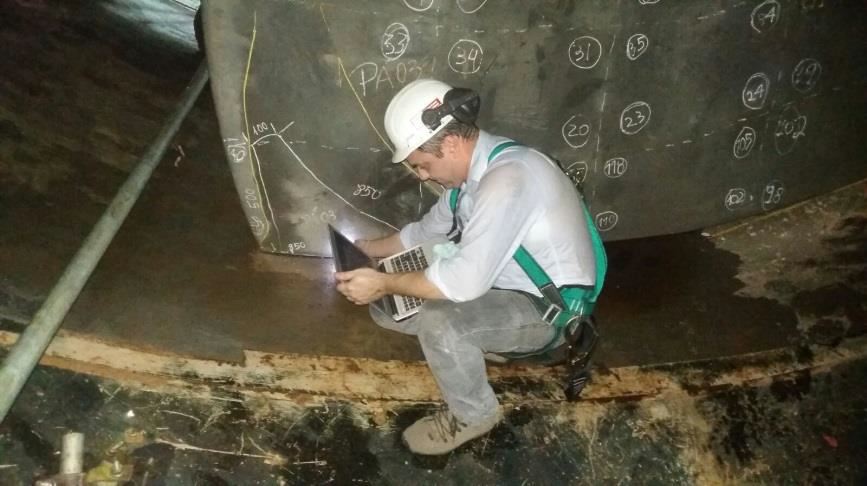
\includegraphics[width=0.9\linewidth, height=4cm]{figs/manolo} 
\caption{A equipe técnica analisa a pá verificando o desgaste do coating
existente e se existem danos a pá em si.}
\label{fig:subim1}
\end{figure}

\begin{figure}[H] 
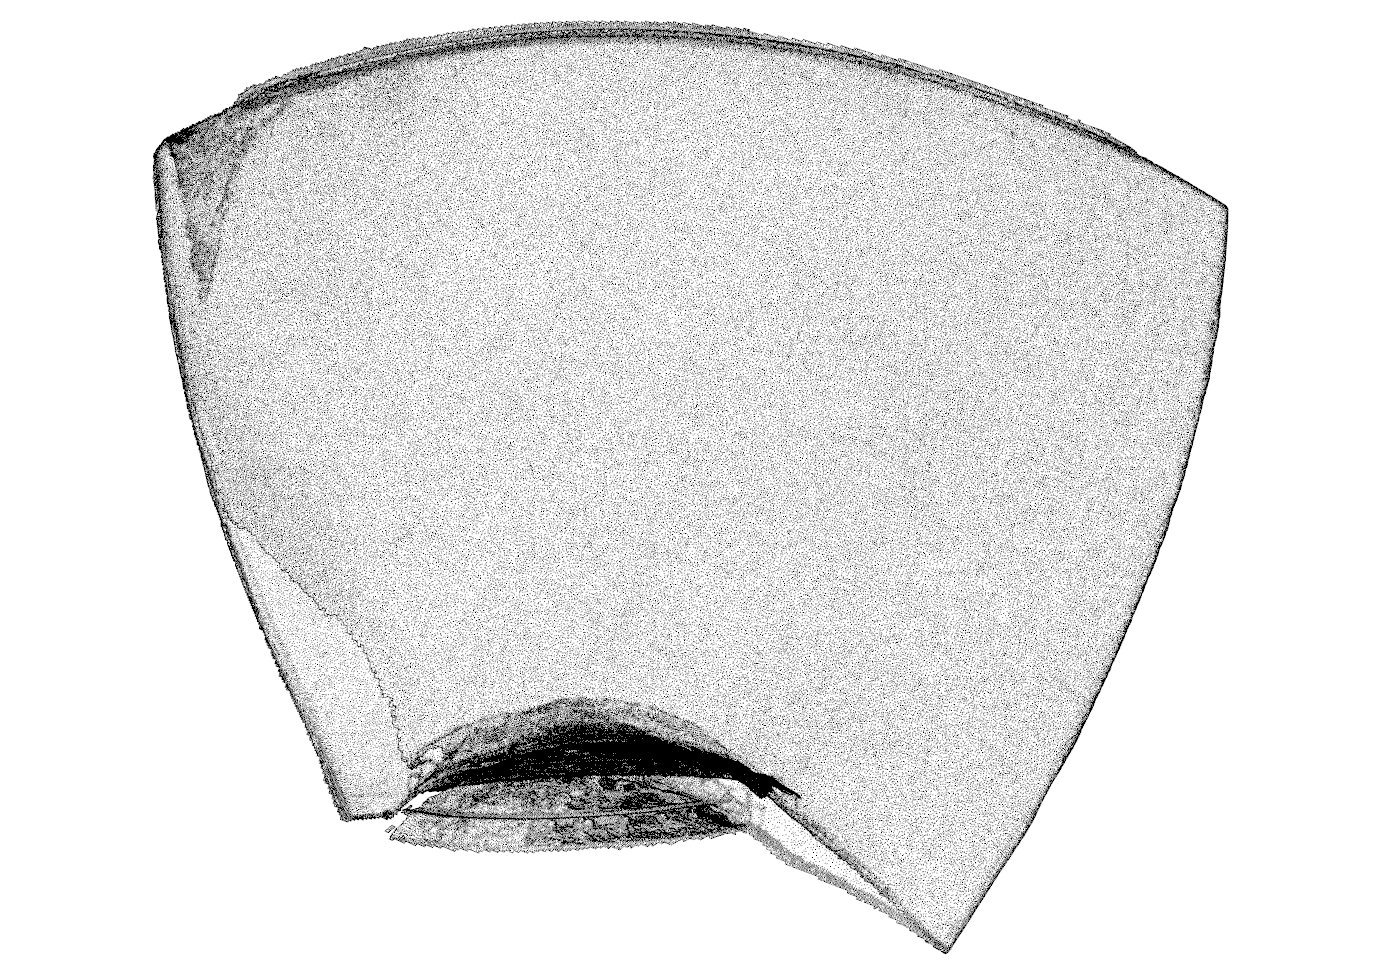
\includegraphics[width=0.9\linewidth, height=4cm]{figs/modelo_pa_faro}
\caption{Dado a necessidade de reparo um laser scanner de metrologia é
utilizado para mapear o dano com uma precisão de 2mm.}
\end{figure}

\begin{figure}[H]
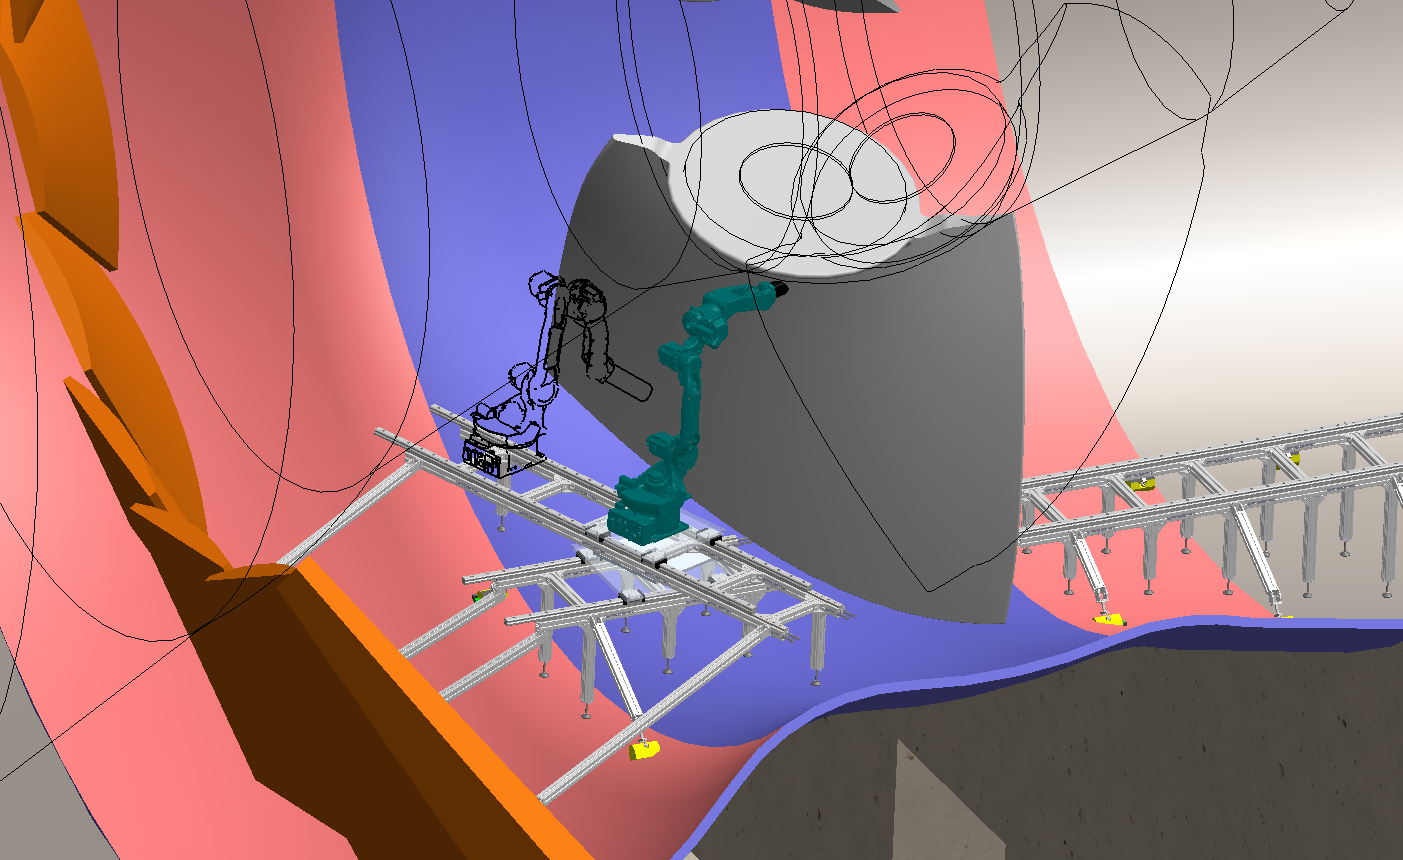
\includegraphics[width=0.9\linewidth, height=4cm]{figs/EMMA_Base_Secundaria_01} 
\caption{Um trilho modular é instalado no ambiente e aconrado através de pinos
magnéticos. O trilho é utilizado para levar o manipulador até a pá e movimentar
o manipulador ao longo da área de trabalho.}
\end{figure}

\begin{figure}[H]
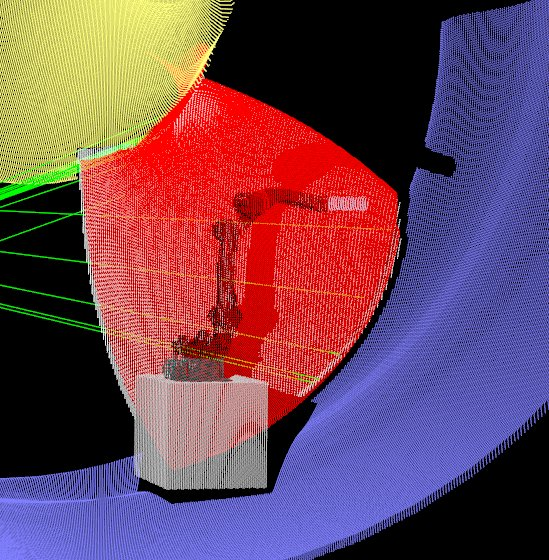
\includegraphics[width=0.9\linewidth, height=4cm]{figs/localizacao}
\caption{Algoritmo de processamento de nuvens de pontos analisam um scan laser
do ambiente e estimam a posição relativa entre o manipulador e a pá.}
\end{figure}


% \begin{figure}[H] 
% \begin{subfigure}{0.5\textwidth}
% 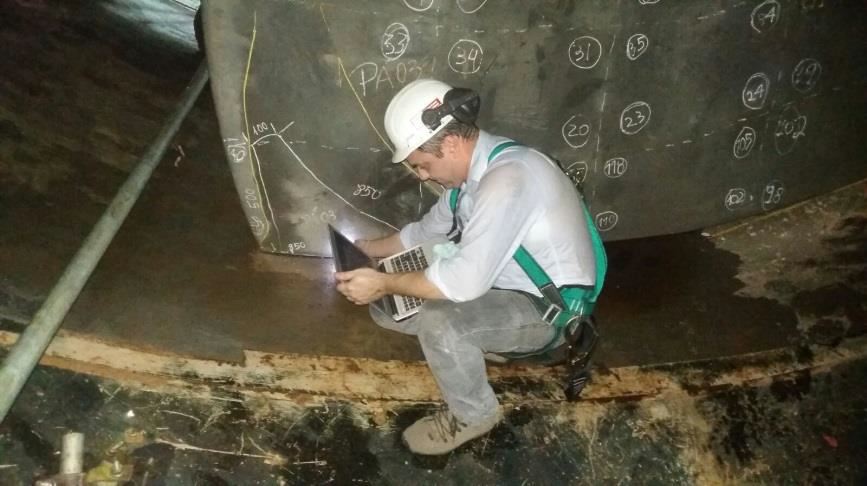
\includegraphics[width=0.9\linewidth, height=4cm]{figs/manolo} 
% \caption{A equipe técnica analisa a pá verificando o desgaste do coating
% existente e se existem danos a pá em si.}
% \label{fig:subim1}
% \end{subfigure}
% ~
% \begin{subfigure}{0.5\textwidth}
% \label{fig:subim2}
% 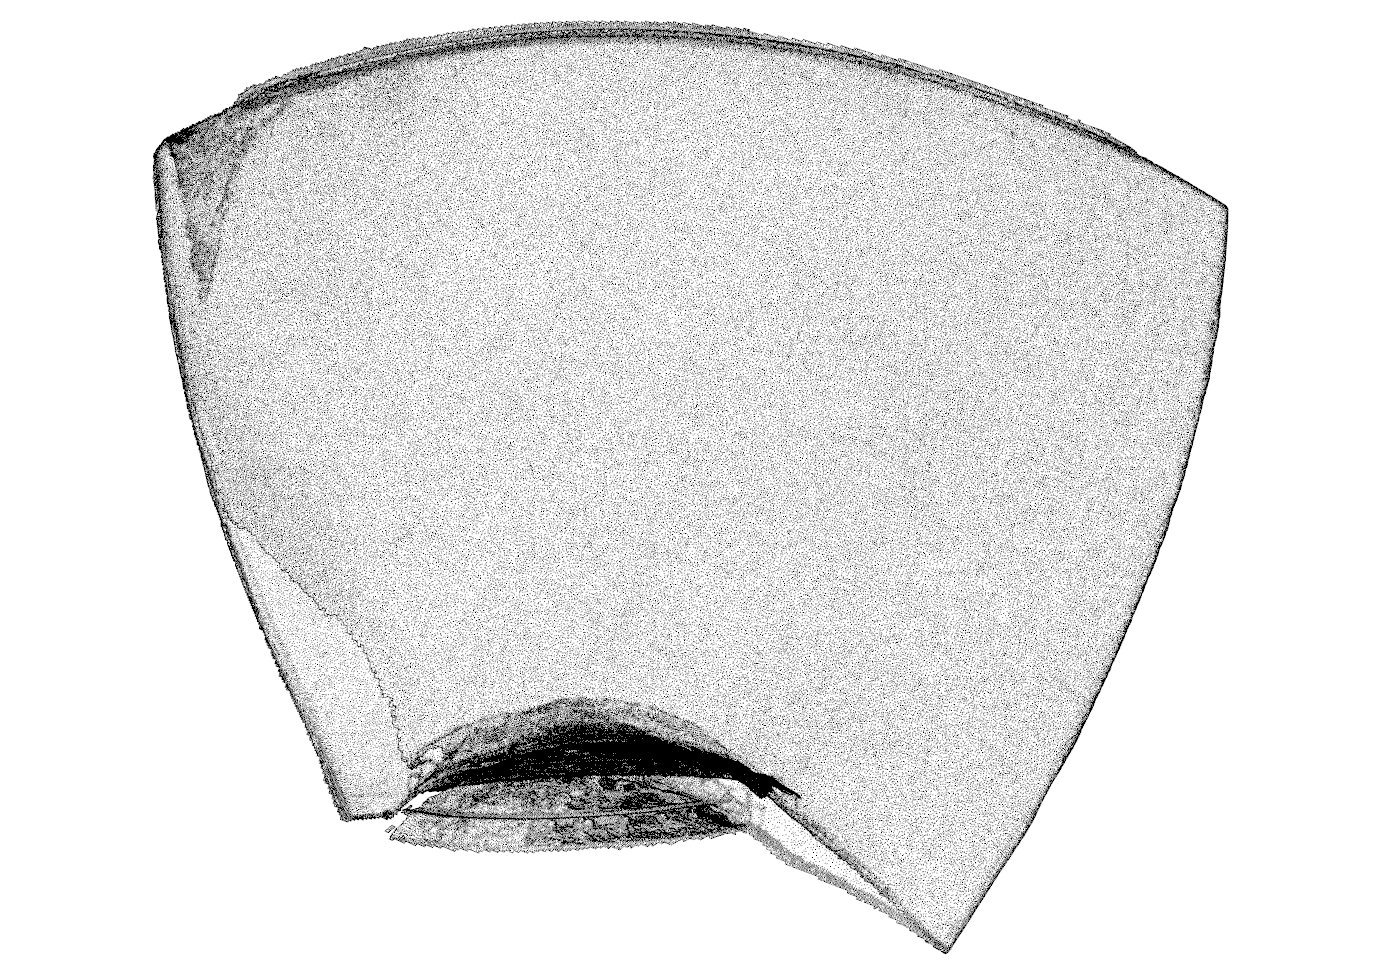
\includegraphics[width=0.9\linewidth, height=4cm]{figs/modelo_pa_faro}
% \caption{Dado a necessidade de reparo um laser scanner de metrologia é
% utilizado para mapear o dano com uma precisão de 2mm.}
% \end{subfigure}
%  \label{fig:image2}
% \end{figure}
% 
% \begin{figure}[H]
% \ContinuedFloat
% \begin{subfigure}{0.5\linewidth}
% 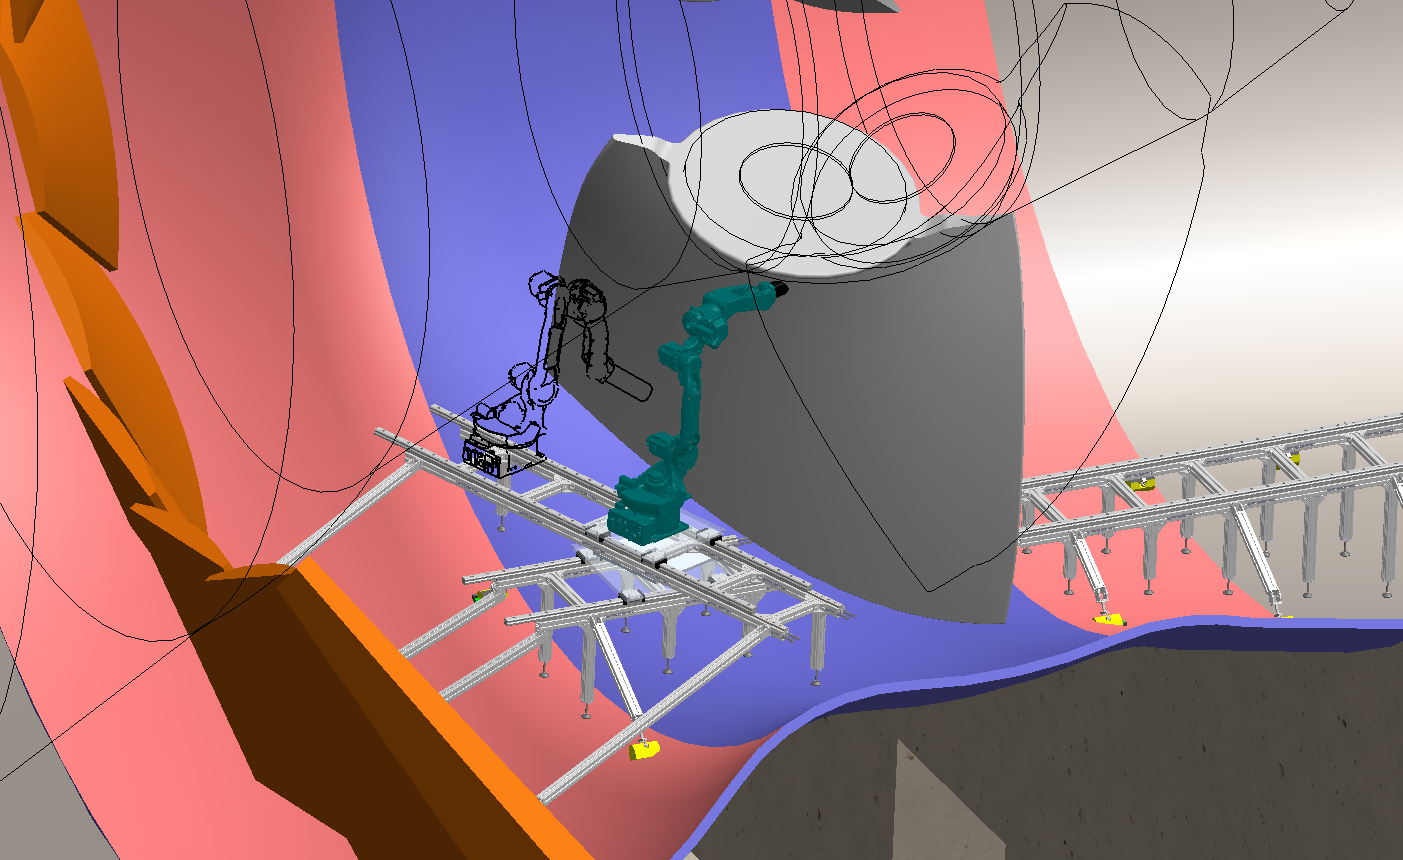
\includegraphics[width=0.9\linewidth, height=4cm]{figs/EMMA_Base_Secundaria_01} 
% \caption{Um trilho modular é instalado no ambiente e aconrado através de pinos
% magnéticos. O trilho é utilizado para levar o manipulador até a pá e movimentar
% o manipulador ao longo da área de trabalho.}
% \end{subfigure}
% ~
% \begin{subfigure}{0.5\linewidth}
% \label{fig:subim2}
% 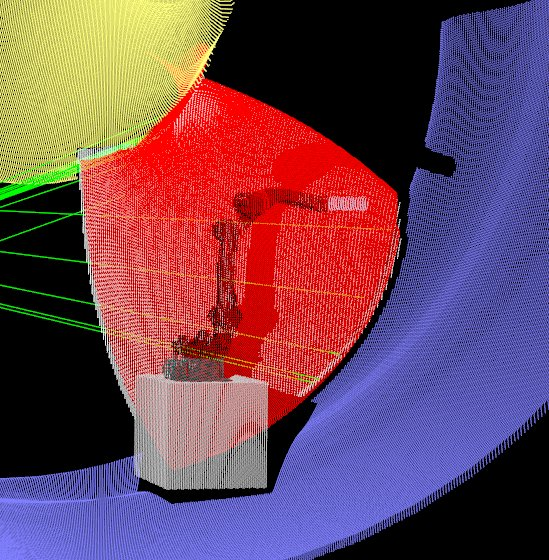
\includegraphics[width=0.9\linewidth, height=4cm]{figs/localizacao}
% \caption{Algoritmo de processamento de nuvens de pontos analisam um scan laser
% do ambiente e estimam a posição relativa entre o manipulador e a pá.}
% \end{subfigure}
%  \label{fig:image2}
% \end{figure}



% \begin{figure}[h!]
% \centering
% \captionsetup[subfigure]{position=b}
% \caption{3D printed wax mould post processing}
% \label{fig:Mould}
% \subcaptionbox{Um trilho modular é instalado no ambiente e aconrado através de pinos
% magnéticos. O trilho é utilizado para levar o manipulador até a pá e movimentar
% o manipulador ao longo da área de
% trabalho.\label{fig:MouldWithSupport}}{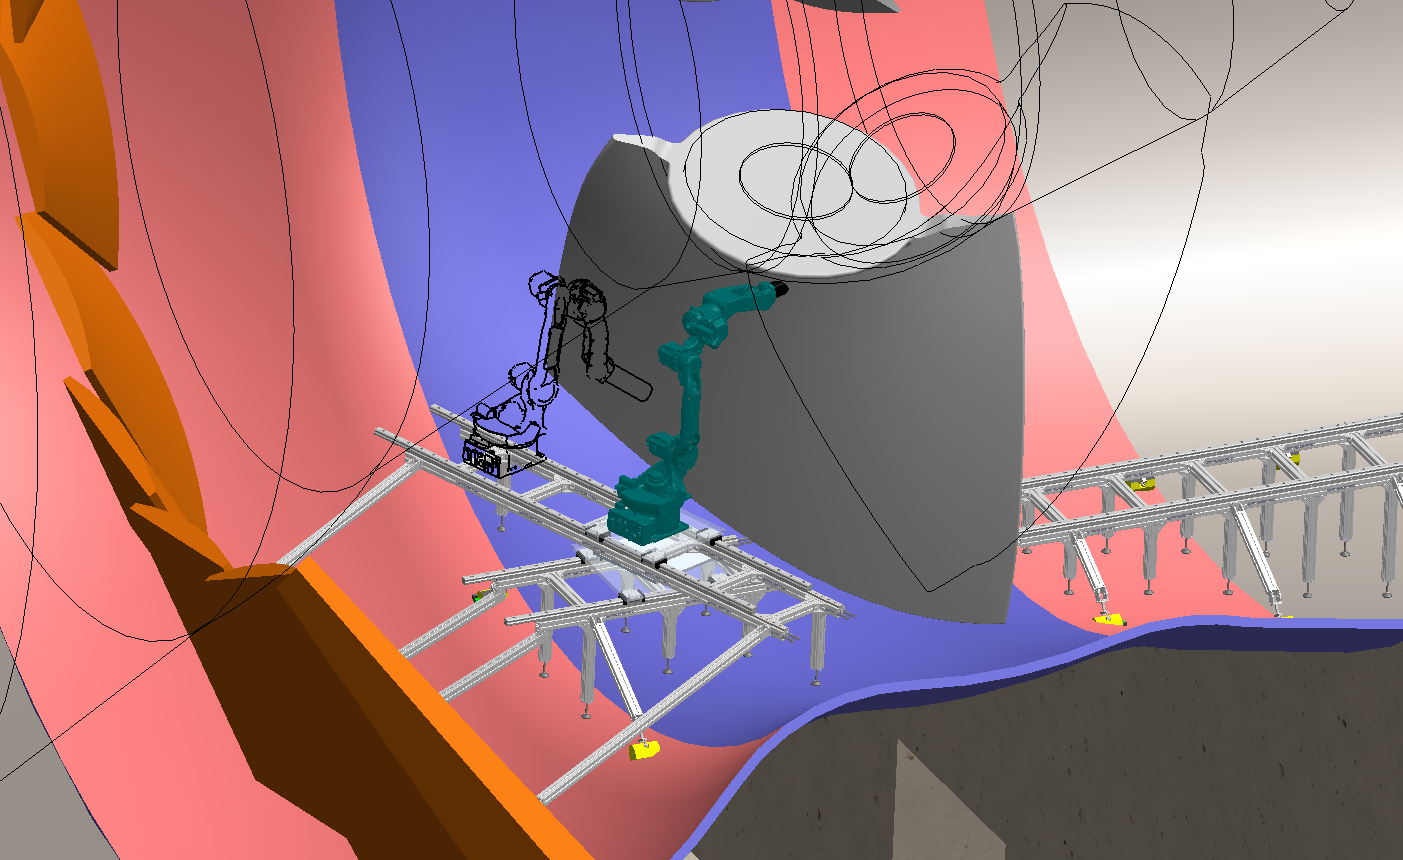
\includegraphics[width=0.5\linewidth, height=4cm]{figs/EMMA_Base_Secundaria_01}}
% \subcaptionbox{Algoritmo de processamento de nuvens de pontos analisam um scan laser
% do ambiente e estimam a posição relativa entre o manipulador e a pá.
% \label{fig:MouldAfterWashing}}{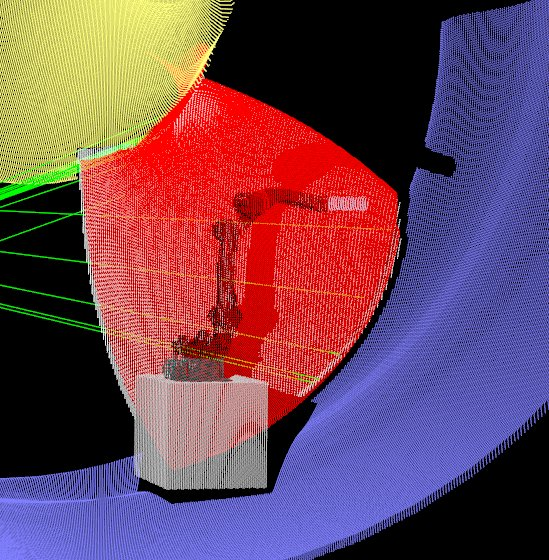
\includegraphics[width=0.5\linewidth, height=4cm]{figs/localizacao}}
% \end{figure}
% \end{document}









\begin{figure}[H]
\ContinuedFloat
\begin{subfigure}{0.5\textwidth}
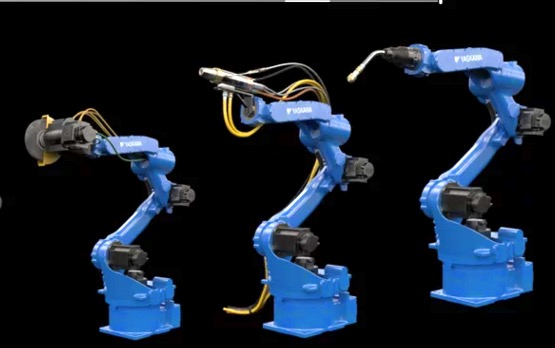
\includegraphics[width=0.9\linewidth, height=4cm]{figs/robots_evo} 
\caption{O equipamento necessário para a tarefa, seja soldagem, esmerilhamento
ou coating é instalado no manipulador e o ambiente e superfície são preparados.}
\end{subfigure}
~
\begin{subfigure}{0.5\textwidth}
\label{fig:subim2}
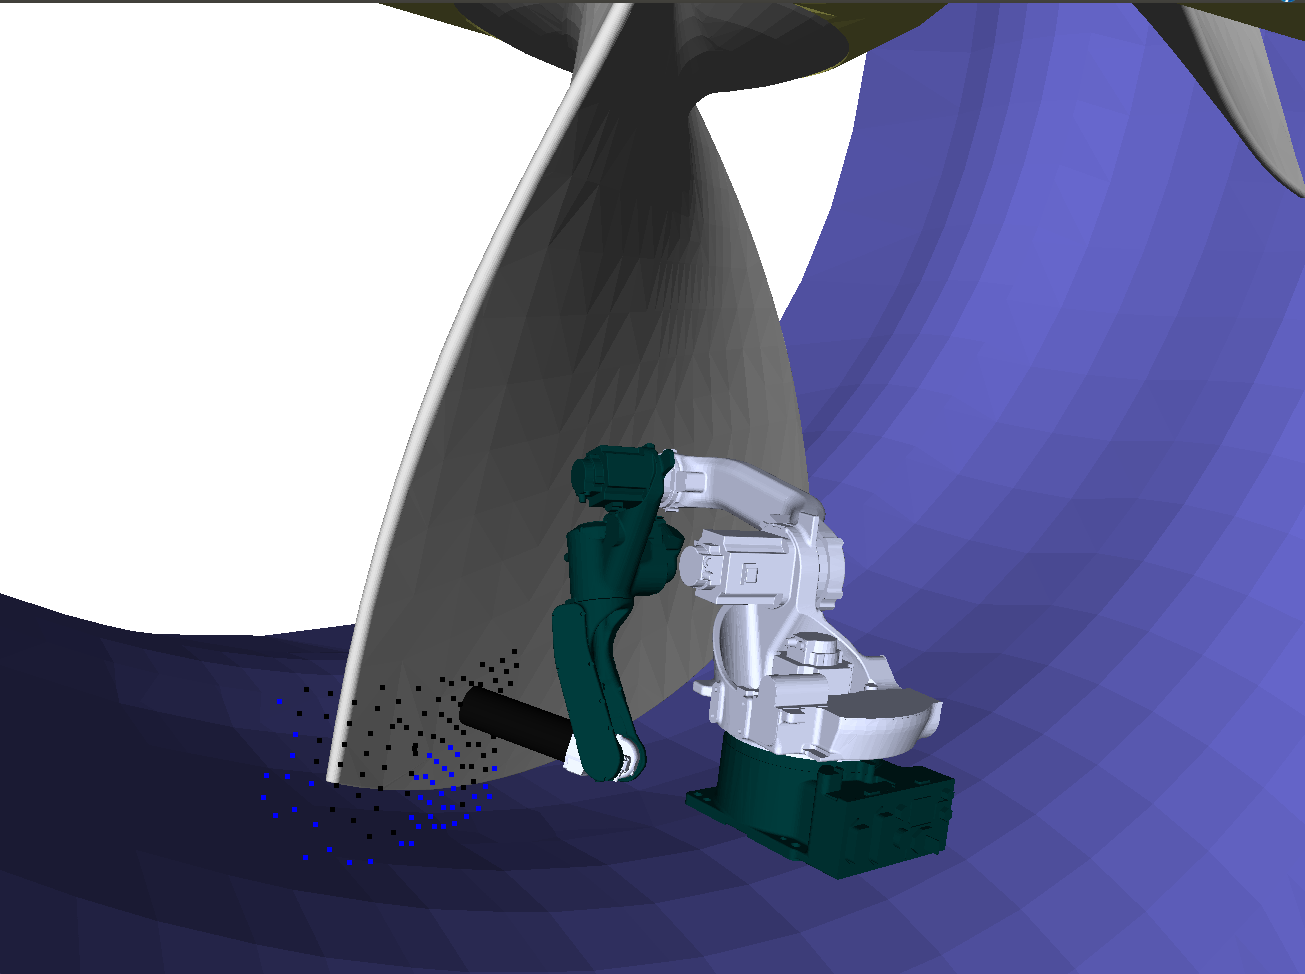
\includegraphics[width=0.9\linewidth, height=4cm]{figs/footleft}
\caption{O algoritmo estima e executa a trajetória para a tarefa planejada.}
\end{subfigure}
 \label{fig:image2}
\end{figure}

O resultado do processo é uma pá restaurada e protegida, aumentando a eficiência
de geração e vida útil da mesma. 

\section{Motivação}

Desgastes por corrosão, erosão e abrasão em pás de turbinas de hidroelétricas
resultam em perda do perfil hidráulico, reduzindo assim a eficiência de geração.
O desgaste reduz também a vida útil da turbina, o tempo de operação entre
paradas de manutenção, assim como, aumentam os custos de manutenção e o tempo
necessário de parada de máquina para a realização do reparo. Logo, significa uma
perda da eficiência de geração, e por consequente um impacto econômico
significativo na operação.
A aplicação de revestimento aumenta a resistência do material contra os
desgastes, custando em torno de 20\% do valor de uma peca nova e representando
um aumento da vida útil em mais de 300\%. Entretanto, dados as limitações da
tecnologia atual, só é possível aplicar o revestimento em bancada, logo, antes
da instalação das pás. Logo, o desenvolvimento tecnológico que possibilite
reaplicar a camada de revestimento dentro do circuito hidráulico resultaria em
um ganho significativo na geração e redução dos custos de operação.
Antes de aplicar o revestimento é necessário reparar a pá recuperando o perfil
hidráulico da mesma, quanto maior a precisão da recuperação do perfil hidráulico
maior a eficiência de geração. Logo, a robótica se torna a ferramenta ideal para a tarefa.

\section{Objetivo}

O objetivo geral do projeto é desenvolver e testar uma metodologia que permita
utilizar a robótica para reparar e revestir pás instaladas em circuitos hidráulicos.

Os objetivos específicos são determinar as metodologias: 

\begin{itemize}
  \item definir o manipulador ótimo para cada hidroelétrica 
  \item movimentar o manipulador dentro do circuito hidráulico
  \item estimar a posição do manipulador com relação ao meio
  \item material e técnica de coating e reparo 
  \item preparar o meio e superfície
  \item logística para instalar um sistema robótico no circuito hidráulico
  \item determinar os riscos associados
  \item planejar e executar a manipulação
  \item representar as diferentes informações do processo para um operador
  \item verificar as perdas de carga do processo de revestimento
  \item integrar e utilizar as diversas ferramentas
  \item mapear o perfil hidráulico e medir os danos
\end{itemize}

\section{Originalidade}

Não existe nenhuma solução ou estudo realizado sobre a aplicação de revestimento
dentro do circuito hidráulico sem desinstalar as pás da turbina. A aplicação de
revestimento para proteção contra abrasão, cavitação, corrosão e erosão em peças
de turbinas de hidrelétricas realizado atualmente é limitada a trabalho em
bancada com a peça desinstalada. O desafio de realizar o trabalho de
revestimento dentro do circuito hidráulico se dá pela dimensão da escotilha de
acesso, que limita o tamanho do robô, pelo posicionamento do robô com relação a
pá da turbina, que se encontra a alguns metros do solo, pelo processo de
aplicação que requer velocidade constante utilizando uma pistola pesada e pelo
controle de temperatura e humidade necessários. Esta pesquisa é inovadora no
setor elétrico brasileiro e é um avanço com relação ao estado da arte.

\section{Aplicabilidade}

A metodologia desenvolvida no projeto  poderá ser aplicada na maioria das
hidroelétricas de médio ou grande porte. A metodologia determina o tamanho e
modelo de manipulador ótimo para o circuito hidráulico em questão, assim como,
qual material de coating a ser aplicado. A restrição para aplicação da tecnologia é
apenas dada pelo espaço entre as pás, em hidroelétricas de pequeno porte a arma
de coating não cabe entre as pás. Logo, a abrangência é nacional, entretanto com
restrição de uso em pequenas unidades geradoras.

\section{Relevância}

A matriz geradora Brasileira é constituída em sua maioria por geração
hidráulica, com um grande número de centrais em rios tipos corredeiras que
possuem reservatórios pequenos. Neste tipo de rio não há tempo de sedimentação
das partículas sólidas na água, essas partículas sólidas, mesmo em quantidades
pequenas, geram um elevado nível de desgaste por erosão e cavitação. Logo, o
projeto é de relevância para o setor elétrico e para a nação, pois aumenta a
eficiência da matriz energética Brasileira, aumenta a disponibilidade da máquina
para geração e reduz os custos de manutenção, representando uma melhora
econômica e social.

\section{Capacitação}

A pesquisa e o desenvolvimento (P\&D) tem como propósito fomentar o avanço
tecnológico e novas maneiras de desenvolver um tipos específicos de conhecimento
no país. O desenvolvimento do EMMA, no âmbito P\&D é um exemplo de como a
parceria entre agências do governo, empresa e universidades podem colaborar para
a capacitação tecnológica e o desenvolvimento de novas tecnologias.

O projeto EMMA possui 4 pesquisadores inscritos no mestrado. Os temas são todos
a pesquisa no campo da robótica, sendo a previsão de conclusão das teses
esperada para a fase 2 e fase 3 do EMMA. Os alunos de mestrado e seus
respectivos cursos são:

\begin{itemize}
  \item Estevão Fróes Ferrão, Programa de Engenharia Mecânica/COPPE, Rio de
  Janeiro
  \item Gabriel Alcantara Costa Silva, Programa de Engenharia Elétrica/COPPE,
  Rio de Janeiro
  \item Eduardo Elael de Melo Soares, Programa de Engenharia Elétrica/COPPE, Rio
  de Janeiro
  \item Julia Ramos Campana, Departamento de Artes e Design, PUC, Rio de Janeiro
\end{itemize}

Para o comprimento dos requisitos de segurança do Ministério do Trabalho e
Emprego, a equipe do projeto foi submetida à capacitação em segurança, nas
normas relevantes às situações encontradas no interior do circuito hidráulico. As certificações foram nas
seguintes normas:

\begin{itemize}
  \item NR10 - Segurança e Instalações e Serviços em Eletricidade
  \item NR33 - Segurança e Saúde nos Trabalhos em Espaços Confinados
  \item NR35 - Trabalho em Altura
\end{itemize}

Os seguintes pesquisadores foram capacitados no curso:

\begin{itemize}
  \item Estevão Fróes Ferrão, Programa de Engenharia Mecânica/COPPE
  \item Gabriel Alcantara Costa Silva, Programa de Engenharia Elétrica/COPPE
  \item Renan Sales de Freitas, Programa de Engenharia Elétrica/COPPE
  \item Eduardo Elael de Melo Soares, Programa de Engenharia Elétrica/COPPE
  \item Julia Ramos Campana %TODO Julia departamento
\end{itemize}
A pesquisa no projeto EMMA proporcionou a elaboração de dois artigos
submetidos/publicados em revistas, abordando os seguintes tópicos: 

\begin{itemize}
  \item Estado da arte e design conceitual de soluções robóticas para
  revestimento de turbinas hidráulicas \textit{in situ} (State of the art and
  conceptual design of robotic solutions for \textit{in situ} hard coating of
  hydraulic turbines).
  \item Solução Conceitual e estudo de viabilidade técnica para para
  revestimento de turbinas hidráulicas \textit{in situ} (EMMA - A robotic
  system for \textit{in situ} hydropower turbine hard coating).
\end{itemize}

\section{Razoabilidade dos Custos}

Atualmente, após a instalação da unidade geradora, não existe método disponível
para proteger a ogiva geradora contra os desgastes de sua utilização. Sendo,
infelizmente, a recuperação sempre o caminho e isso pode ser estimado entre 90 e
120 dias de UG parada. A frequência de paradas de recuperação variam dependendo
da idade da unidade geradora, material, tipo de bacia e etc. A única certeza é
que um dia será necessário. A aplicação de revestimento pode ser realizada
durante as paradas planejadas, sem perda de tempo de geração.
De acordo com a tabela de situação de cavitação em turbina hidráulica no Brasil
(Out/97), em média 5 unidades geradoras apresentaram  cavitação a cada 24.071
horas de operação (2,7 anos), das 36 instalações analisadas. Logo, em Jirau a
aplicação do revestimento in situ significaria em um aumento da disponibilidade
de geração de 600 dias a cada 2,7 anos, considerando turbinas de 75 MW de
potencia, seria equivalente a 1.080.000 MW a cada 2,7 anos.

\section{Metodologia adotada}

O projeto EMMA foi dividido em 3 fases, sendo cada fase um projeto distinto.
Cada fase avançando a tecnologia ao longo da cadeia de inovação. Na primeira
fase foi desenvolvido a metodologia/conceito. Na segunda fase será feito o
desenvolvimento experimental testando o sistema de coating. Na terceira fase
será expando a solução para incluir reparo e validar a tecnologia em outras
centrais hidroelétricas.

Ao início da primeira fase não se sabia se existiria uma solução para o
problema. Os requisitos de acesso, operação e coating são extremamente
limitantes. A metodologia adotada na fase 1 para desenvolver o conceito da
solução foi:

\textbf{Etapa 1}: Levantamento dos requisitos do ambiente, tarefas e
procedimentos.
Estudo do estado da arte e bibliografias existente no tópico. Baseado nos
requisito e estado da arte foi definido uma solução conceito que atende ao problema.

\textbf{Etapa 2}: A solução conceito foi detalhada. Neste detalhamento foi
determinando os equipamentos e fornecedores que seriam adequados a serem
utilizados na solução. Assim como foi realizado pesquisa bibliográfica para
determinar quais os algoritmos e técnicas mais adequadas a serem implementadas
como parte da solução.

\textbf{Etapa 3}:  A solução conceito detalhada foi validada através de
simulações e experimentos em laboratório de alguns conceitos chaves. Um exemplo
foi utilizar o openrave para simular o processo de movimento do manipulador e
experimentos de campos da fixação por pino magnético.

\section{Estratégia de difusão}

A estratégia de difusão adotada no projeto foi a realização de um evento de
transferência de conhecimento dentro da faculdade de porto velho que inclui não
apenas os funcionários da ESBR, mas também os alunos e professores da faculdade.
O evento serviu como um “aulão” em pesquisa aplicada em robótica. Onde cada
pesquisador do projeto, em sua maioria alunos de mestrado da UFRJ, deram uma
aula sobre seus tópicos de pesquisa dentro do projeto.

%TODO foto do evento

\section{Melhorias de processo, equipamento e sistema}

O projeto representa uma melhoria no processo de reparo das pás de turbina
hidroelétricas que atualmente são feitas manualmente. Espera-se que o processo
robótico consiga recuperar o perfil hidráulico para uma margem de 2-5 mm do perfil original.

O fato de o EMMA também realizar o revestimento das turbinas instaladas, algo
antes impossível, o projeto representa uma melhoria no equipamento (pás das
turbinas), pois as mesmas se tornam mais resistentes aos danos corrosão, erosão e abrasão.

Por fim, o projeto também representa uma melhoria a todo sistema de geração de
energia elétrica. Pois, aumenta a vida útil das turbina e mantêm o perfil
hidráulico original, logo um impacto direto no aumento da geração.

\section{Pesquisa Correlatas}

\textbf{Google Schoolar, IEEE, Field Robotics, ... }: nenhum resultado foi
encontrado na revisão bibliográfica para uma solução robótica de aplicação de
revestimento em turbinas hidroelétrica já instaladas no Brasil e no exterior. A
pesquisa revela apenas o desenvolvimento de robôs para reparos in situ da
turbina, capazes de realizar soldagem, em exemplo RoboTurb da UFSC e Scompi da
Hydro-Quebec. Ambos não aplicáveis ao problema de revestimento devido as
limitações do manipulador robótico nos sistemas.

\textbf{INPI}: Nenhuma patente foi encontrada que se enquadre como o produto
objeto da pesquisa e desenvolvimento aqui proposta.

\textbf{ANEEL}: nenhum resultado foi encontrado na base de dados da ANEEL
relevante a um robô para revestimento. Os resultados encontrados referiam-se a
um Robo que inspeciona e corrige problemas em linhas de transmissão; Sistema
Multi-robôs Aéreos para Inspeção de Linhas e Robô para Inspeção Visualde
caldeiras.

\section{Instituição e Equipe}

O LEAD (Laboratório de Controle e Automação, Engenharia de Aplicação e
Desenvolvimento) é fruto de uma parceria entre a Petrobras e a Universidade
Federal do Rio de Janeiro (UFRJ) que visa ao desenvolvimento de novas
tecnologias na área de Automação e Controle.
Na avaliação da estatal brasileira de petróleo, ‘‘o laboratório reforça a
estratégia de desenvolvimento em conjunto de novas tecnologias, o que traz
benefícios tanto para as universidades, que realizam suas pesquisas acadêmicas
em laboratórios de ponta, quanto para a Petrobras que, ao compartilhar
conhecimentos, cria competências para superar seus desafios tecnológicos e
empresariais”.

DARLAN PARAGRAFO RIJEZA

%TODO DARLAN PARAGRAFO RIJEZA

A equipe técnica alocada para a realização do projeto EMMA:

\begin{itemize}
  \item Renan Salles de Freitas, Engenheiro de Controle e
Automação pela UFRJ, Rio de Janeiro, Brasil, e Candidato a Mestre em Ciências em Engenharia Elétrica
pelo Programa de Engenharia Elétrica, COPPE/UFRJ, Rio de Janeiro, Brasil. No
projeto EMMA, Renan é membro da equipe de Controle e Robótica, e responsável
pelas seguintes atividades: Manipuladores industriais: pesquisa de
mercado, análise cinemática, dinâmica e controle; Desenvolvimento do ambiente de
simulação para análise de soluções; Análise de viabilidade técnica do EMMA pela
visão da robótica e do controle; Desenvolvimento e simulação de algoritmos de
planejamento de trajetória.

  \item Estevão Fróes Ferrão possui graduação em Engenharia Mecânica pela Universidade
Federal do Rio de Janeiro (UFRJ), atualmente cursando o mestrado no Programa de Engenharia
Mecânica (PEM-COPPE/UFRJ). Faz parte da equipe do Projeto EMMA, como
Pesquisador/Engenheiro contratado pelo LEAD. Atua na área de Projeto Mecânico,
sendo resposável pela pesquisa, projeto e desenvolvimento de uma solução
mecânica para uma base com graus de liberdade que permitem o posicionamento do
robô utilizado.

\item Julia Ramos Campana é formada em Comunição Técnica e Mídia pelo Instituto de
Tecnologia e Illinois, pós graduada em Design Digital pela Vancouver Film School
e em Gerenciamento de Projeto pela Universidade da Columbia Britânica, é
atualmente aluna do Mestrado em Design pela PUC-RJ. Julia exerce a função de
Designer de interface e Usabilidade no projeto EMMA, trabalhando no
desenvolvimento do software de controle do sistema EMMA e em todas as questões
relacionadas aos usuários, testes e interações humano-automação da pesquisa.
\item Eduardo Elael de Melo Soares, Engenheiro de Controle e Automação pela UFRJ, Rio
de Janeiro, Brasil, e mestrando em Ciências em Engenharia Elétrica pelo
Programa de Engenharia Elétrica, COPPE/UFRJ, Rio de Janeiro, Brasil. No projeto
EMMA, Eduardo é membro da equipe de Controle e Robótica, e responsável pelas
seguintes atividades: Manipuladores de pequeno porte: Pesquisa e análise
geométrica; Realimentação de segurança: Pesquisa de laser 1D para uso em tempo
real; Reconhecimento de ambiente: Escolha e adaptação de técnicas para
reconhecimento da posição do Robô no ambiente; Desenvolvimento e simulação de
algoritmos de planejamento de trajetória.
\item Gabriel Alcantara Costa Silva, Engenheiro de Controle e Automação pela
UFRJ, Rio de Janeiro, Brasil, e mestrando em Ciências em Engenharia Elétrica pelo
Programa de Engenharia Elétrica, COPPE/UFRJ, Rio de Janeiro, Brasil. No projeto
EMMA, Eduardo é membro da equipe de desenvolvimento de software para sistemas
robóticos, e responsável pelas seguintes atividades: Desenvolvimento de técnicas
em visualização, localização e mapeamento 3D; Identificação e
Localização de objetos; Integração do sistema.

\end{itemize}








    
    
  


\chapter{Plano de Projeto}\label{chap::planejamento}


\section{Etapa 1 - Fundação Coppetec}

\begin{figure}[H]
\centering
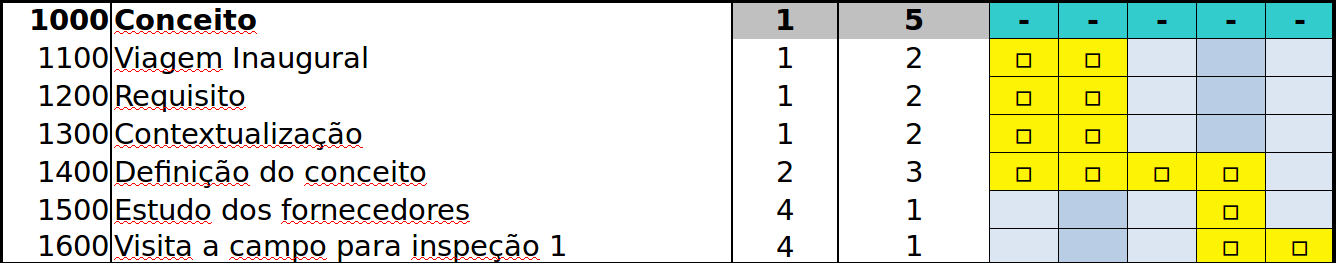
\includegraphics[width=0.9\columnwidth]{figs/etapa1_completo}
\end{figure} 

\textbf{1000 Conceito:} A etapa 1000 do projeto foi executada como prevista. O
objetivo da etapa foi a determinação dos requisitos do problema e concepção de
possíveis soluções. As seguintes trabalhos foram executados dentro desta etapa

\noindent
\textbf{1100 Viagem Inaugural:} Assinatura do termo inaugural do projeto e
análise em campo da problemática

Etapa executada como previsto. 

\begin{figure}[H]
\centering
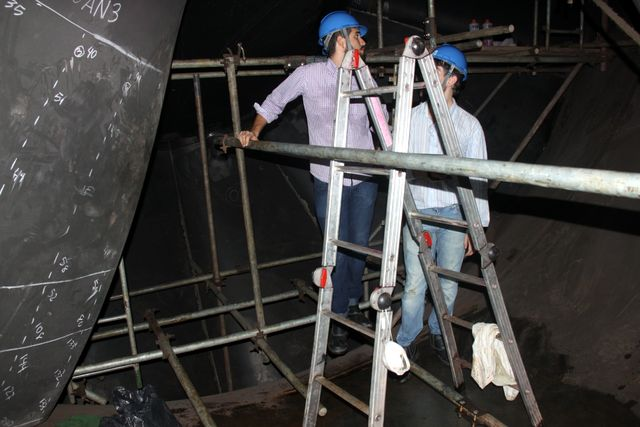
\includegraphics[width=0.6\columnwidth]{figs/img_4967}
\caption{Pesquisadores analisando o ambiente.}
\end{figure}

\noindent
\textbf{1200 Requisito:} Fazer levantamento dos requisitos que afetam a
instalação e utilização de um robô dentro circuito hidráulico.

Etapa executada como previsto. Foram levantados todos os requisitos de acesso,
ambiente e processo de coating.

\noindent
\textbf{1300 Contextualização:} Levantamento das tecnologias existentes no para
aplicações de revestimento em ambientes confinados.

Etapa executada como previsto. Diversas tecnologias foram pesquisadas, como o
robô scompi da hidroquebec. Nenhuma das soluções atuais atendiam os requisitos
de operação do projeto.

\noindent
\textbf{1400 Definição dos conceitos:} Definição de uma solução de um robô capaz
de operar no ambiente e realizar tarefas de revestimento.

Etapa executada como previsto. Foram levantados 3 conceitos viáveis, os quais
foram analisados chegando ao conceito proposto dentro do projeto. Utilizar um
manipulador industrial, acessando o circuito hidráulico pela escotilha de
acesso, com movimentação através de trilhos modulares e alinhamento, mapeamento
e planejamento de trajetória baseado em scan 3D a laser do ambiente.

\begin{figure}
\centering
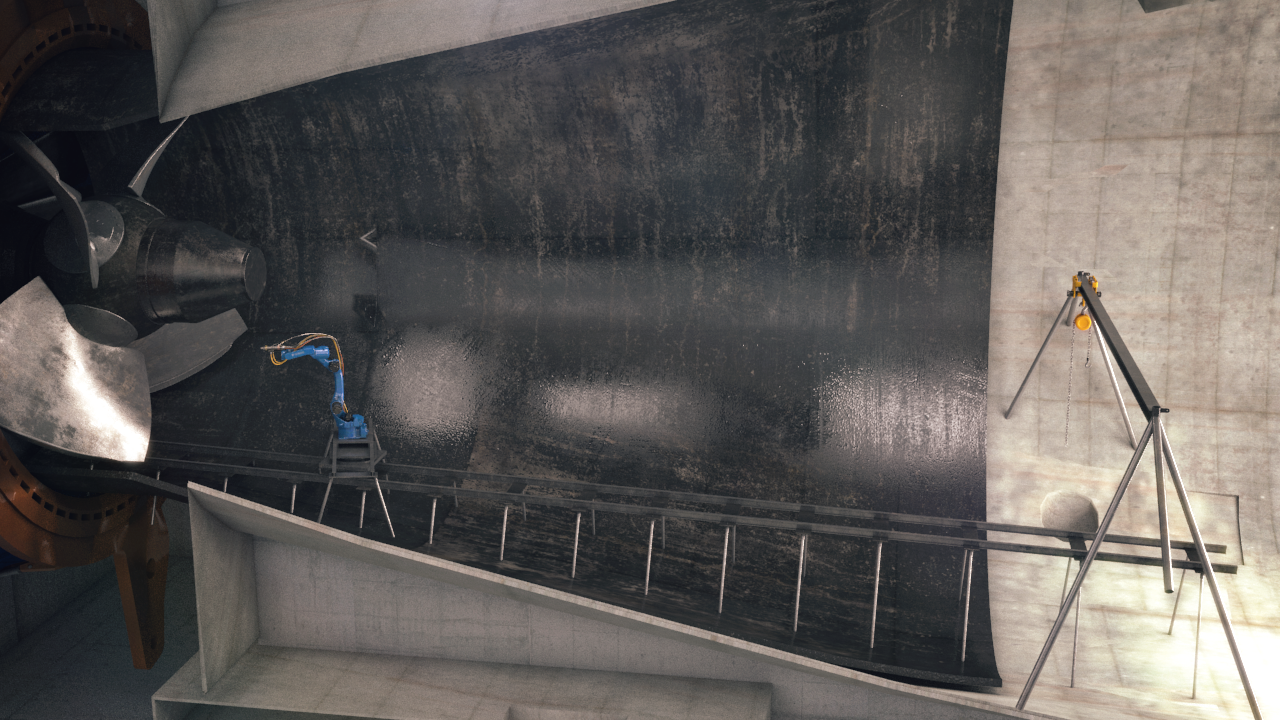
\includegraphics[width=0.9\columnwidth]{figs/turbine_evo}
\caption{Solução conceito.}
\end{figure}

\noindent
\textbf{1500 Estudo dos fornecedores:} Definição dos fornecedores do equipamento
necessário para a pesquisa

Etapa executada como previsto. Foram analisados mais de 50 modelos de
manipuladores distintos, sendo que 5 atendiam os requisitos do problema como
possíveis soluções.

\begin{figure}[h!]
\centering
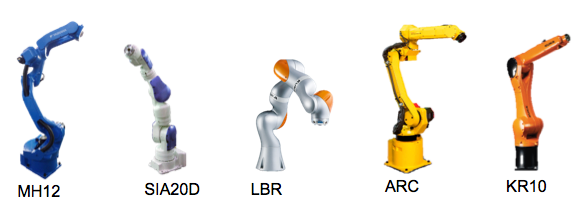
\includegraphics[width=0.9\columnwidth]{figs/robots}
\caption{Possíveis modelos de manipuladores que atendem os requisitos.}
\end{figure}

\noindent
\textbf{1600 Visita a campo para inspeção 1:} foi realizada uma visita inicial
a campo para juntamente com revisão bibliográfica sobre o tema “desgaste”
coletar dados de campo através de inspeção nas pás das turbinas. Essas inspeções
foram realizadas ao longo do projeto para confrontar com o que existe na
bibliografia.


\section{Etapa 02}

\begin{figure}[H]
\centering
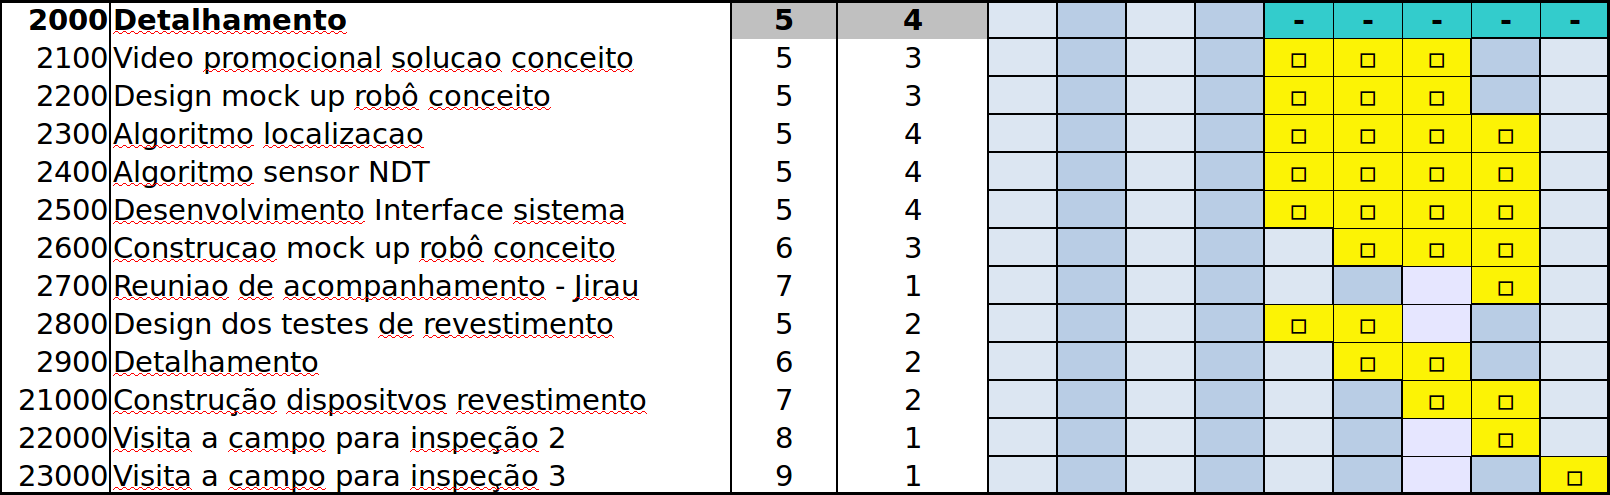
\includegraphics[width=0.9\columnwidth]{figs/etapa2_completo}
\end{figure} 

\noindent
\textbf{2000 Detalhamento:} A etapa 2000 do projeto foi executada existindo
variações entre previsto e executado. O objetivo da etapa foi a análise das
proposições mediante estudos teóricos e design detalhado da possível solução e sistema

\noindent
\textbf{2100 Video promocional solução conceito:} Animação 3D da solução
conceito

Houve atraso no processo de contratação e aprovação do script. A tarefa foi
executada com 3 meses de atraso. Entretanto, o mesmo não impactou no projeto,
pois não era uma tarefa de pré-requisito.

\noindent
\textbf{2200 Design mock up robô conceito:} Design em CAD / Solidworks do
conceito do robô

Tarefa executada como prevista. Foram realizado diversos designs para possíveis
bases para a solução conceito, assim como análises geométricas, cinemática,
dinâmica e de manipulabilidade para definir o manipulador.

\begin{figure}\centering
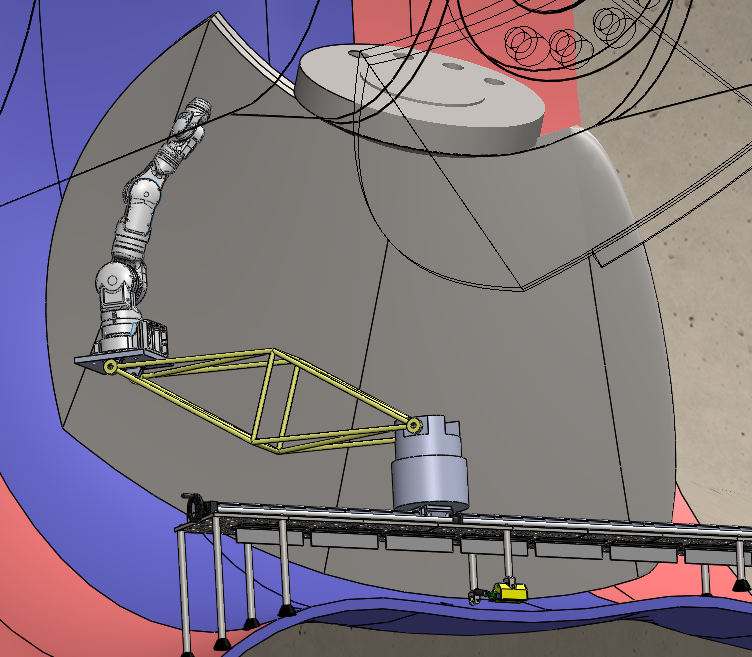
\includegraphics[width=0.6\columnwidth]{figs/EMMA_Base_Conceito_PRR}
\caption{Possível base para o manipulador dentro do ambiente do circuito
hidráulico.}
\end{figure} 


\noindent
\textbf{2300 Design dos testes de revestimento:} %TODO DARLAN

\noindent
\textbf{2400 Algoritmo de localização:} definir o algoritmo/técnica que irá
localizar o robô com relação a turbina.

Tarefa executada como prevista. Foi determinado que o melhor e mais preciso
método é escanear o robô e a pá com um laser de metrologia e a estimar posição
relativa das nuvens de pontos resultantes.

\begin{figure}[H]
\centering
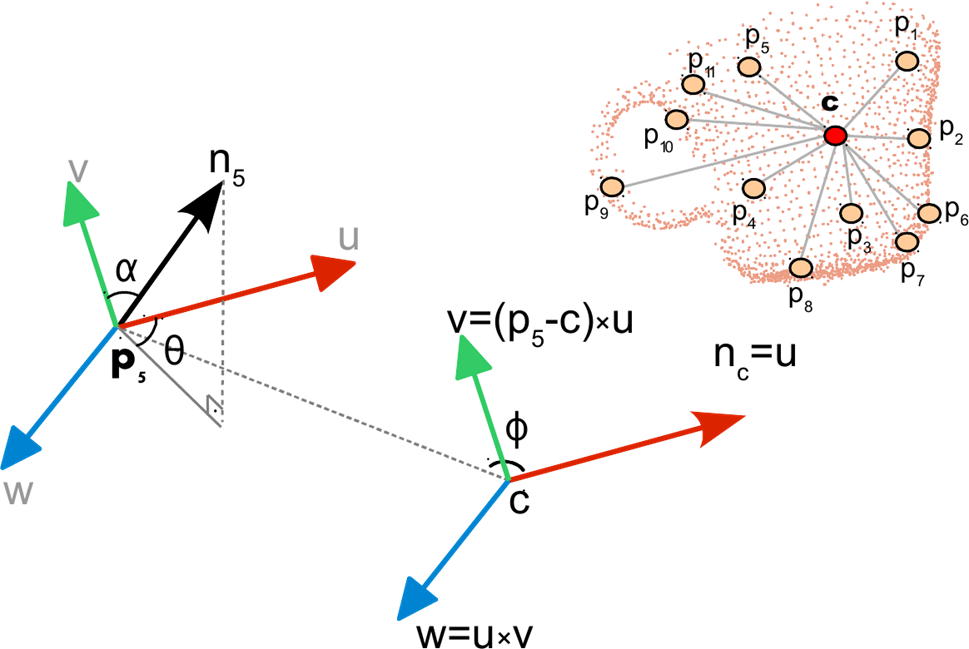
\includegraphics[width=0.6\columnwidth]{figs/pc_position}
\caption{Posição relativa entre duas nuvens de pontos.}
\end{figure} 

\noindent
\textbf{2500 Algoritmo sensor NDT:} Algoritmo que irá avaliar e mapear a
qualidade do revestimento.

Tarefa executada como prevista. Foi determinado que o método mais eficiente é
utilizar um humano para rapidamente realizar uma amostragem de alguns pontos com
sensor ultra-som manual. A solução robótica seria em uma alusão “matar um mosquito com basuca”.

\noindent
\textbf{2600 Desenvolvimento Interface sistema:} Interface gráfica de controle e
utilização do sistema

Essa tarefa foi estendida para 8 meses, se tornando uma teses de mestrado dada
sua complexidade. A solução conceito possui um volume muito grande de interação
e informação para o usuário. Logo, adotou-se um estudo metódico,
estabelecendo-se toda a metodologia para determinar a interface e como cada
informação será representada.

\noindent
\textbf{2700 Construção mock up robô conceito:} Construção do mock up do robô
que aplica o revestimento

Tarefa executada como previsto. Foi construído todo o ambiente do circuito
hidráulico e manipulador através de impressão 3D em uma escala 1:20.

\begin{figure}[h!]
\centering
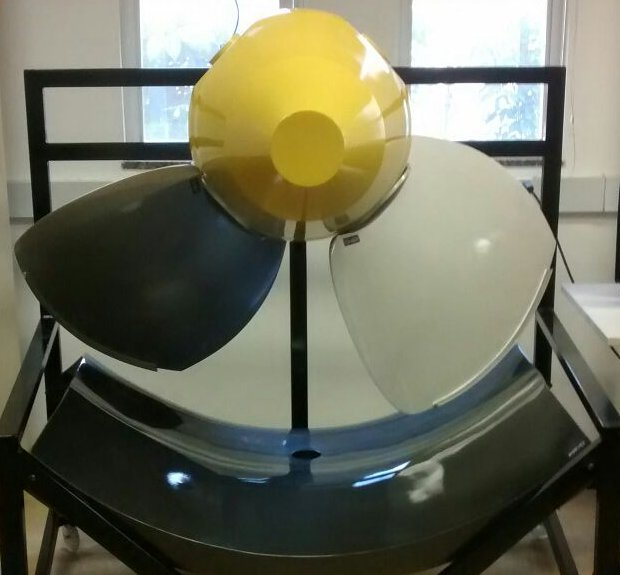
\includegraphics[width=0.6\columnwidth]{figs/maquete}
\caption{Maquete utilizada no desenvolvimento do conceito.}
\end{figure} 

  
\noindent
\textbf{2800 Design dos testes de revestimento:} %TODO DARLAN

\noindent
\textbf{2900 Reunião de acompanhamento:} Reunião de acompanhemento do projeto.
Tarefa executada como prevista.

\noindent
\textbf{21000 Construção dispositivos revestimento:}


\noindent
\textbf{22000 Visita a campo para inspeção 2:}


\noindent
\textbf{23000 Visita a campo para inspeção 3:}

\begin{figure}\centering
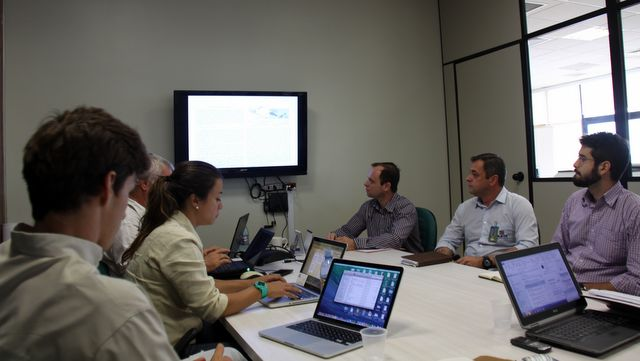
\includegraphics[width=0.6\columnwidth]{figs/img_4836}
\caption{Reunião de acompanhamento em Jirau.}
\end{figure} 

\section{Etapa 03} 

\begin{figure}[H]
\centering
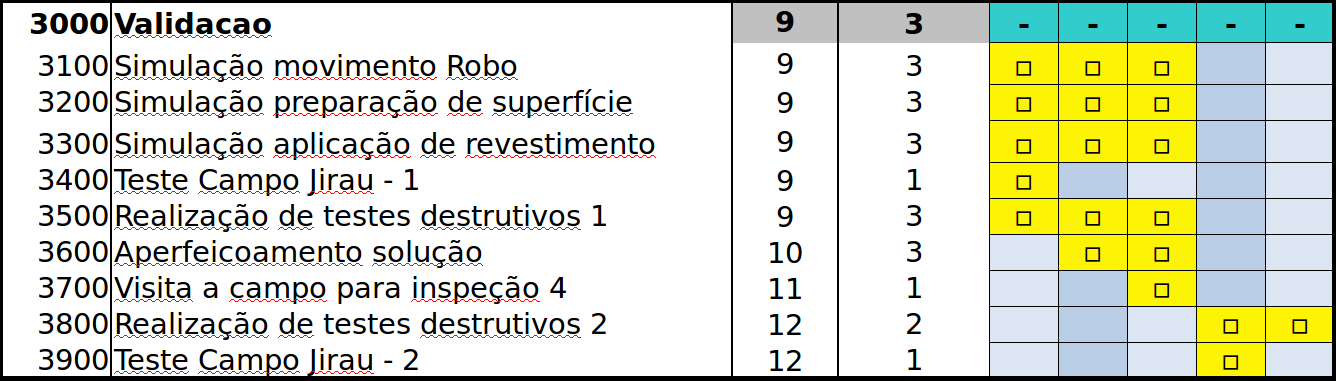
\includegraphics[width=0.9\columnwidth]{figs/etapa3_completo}
\end{figure} 

\noindent
\textbf{3000 Detalhamento:} A etapa 3000 do projeto foi executada existindo
variações entre previsto e executado. O objetivo da etapa é validação da solução
detalhada através de simulação e experimentos.

\noindent
\textbf{3100 Simulação movimento robô:} 
Simulação dos movimentos do robô sobre a turbina, verificando limites e singularidades

Tarefa executada como prevista. Foi utilizado o simulador Openrave.  

\noindent
\textbf{3200 Simulação preparação de superfície:}
Testes para avaliar a modificação do procedimento de jateamento para a sua adequação ao ambiente proposto no projeto;

\noindent
\textbf{3300 Simulação aplicação revestimento:}

Aplicação em amostras de testes para qualificação de materiais e procedimento de aspersão para posterior avaliação comparativa do desempenho dos sistemas de revestimentos.


\noindent
\textbf{3400 Teste de Campo Jirau 01:} Teste da solução  em Jirau sobre
condições reais de operação

Tarefa executada antes do previsto. Os testes de campo foram executados durante
a viagem de acompanhamento que ocorreu na etapa 2900. Foram testados os
conceitos de acoplamento magnético e mapeamento 3D com laser scanner.
\begin{figure}
\centering
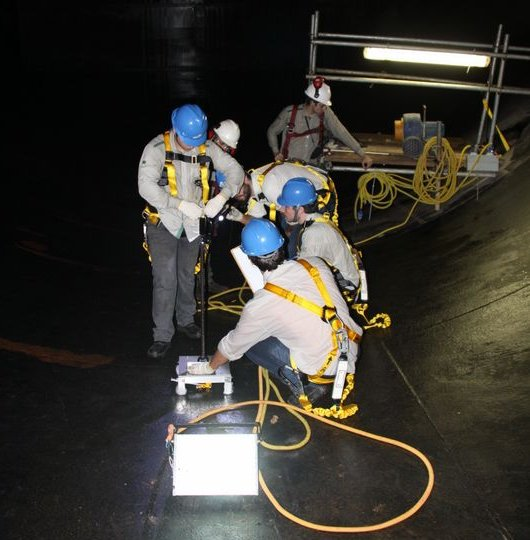
\includegraphics[width=0.6\columnwidth]{figs/base}
\caption{Teste de campo com a base  magnética}
\end{figure}

\noindent
\textbf{3500 Realização dos testes destrutivos – 1}
Realização dos testes para verificar se o revestimento mantém as 
características técnicas exigidas para a aplicação após mudanças de parâmetros. Nessa etapa foram realizados os testes de qualificação dos revestimentos antes e após mudanças de parâmetros e realização de ensaios destrutivos comparativos normatizados. 

\noindent
\textbf{3600 Aperfeiçoamento da solução:}
Aperfeiçoamento da solução baseado nos resultados dos testes de campo 

Tarefa atrasada em 1 mês com impacto de atraso de 1 mês no projeto. O cálculo da
posição relativa entre o robô e a pá, baseado em dados reais do sensor de
metrologia testado em campo, está com um erro de 0,1-0,2 graus o que resulta em
um erro de posição da extremidade do manipulador na ordem de centímetros. A
ordem de grandeza desejada para poder fazer reparo do perfil hidráulico é em
milímetros. Logo, as técnicas de alinhamento continuando sendo aprimoradas.

\begin{figure}\centering
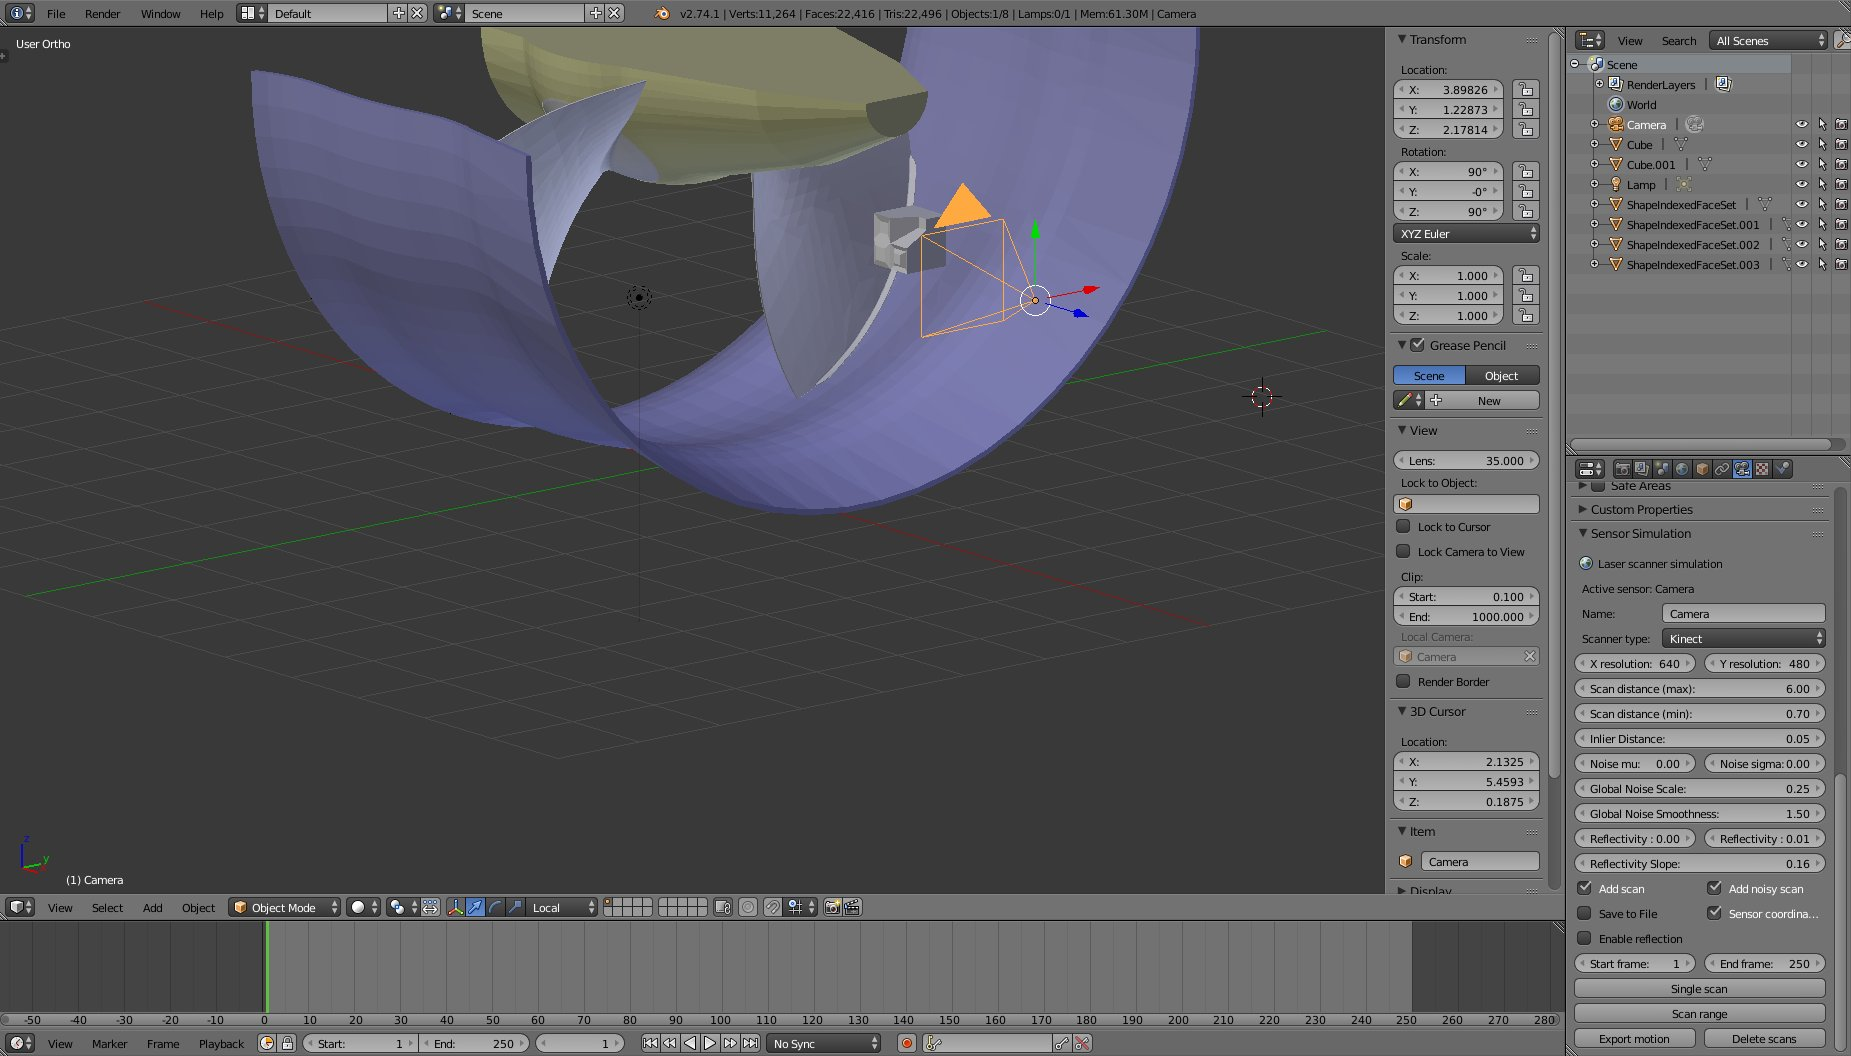
\includegraphics[width=0.6\columnwidth]{figs/blensor_screen}
\caption{Estimando posição relativa usando um simulador para análise dos
resultados.}
\end{figure} 


\noindent
\textbf{3700  Visita a campo para Inspeção 4:}
A inspeção nas pás é realizada com o fim de avaliar o progresso do desgate nas superfícies das pás e também determinar o tipo e a severidade em cada região da pá. 

\noindent
\textbf{3800 Realização dos testes destrutivos 2:}

Continuação da realização dos testes destrutivos após anális dos resultados prévio. As amostras que estvam em atraso na antrega dos resultados de cavitação foram realizadas nessa etapa. Também foram testes de aplicação de revestimento orgânico para melhoria das características do revestimento.


\noindent
\textbf{3900 Teste de Campo Jirau 02:} Teste da solução  em Jirau sobre
condições reais de operação.

Tarefa cancelada. As informações necessárias para esta fase do
projeto foram coletadas durante o teste de campo 01. 

\section{Etapa 04} 

\begin{figure}[H]
\centering
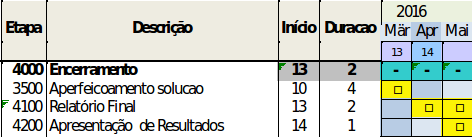
\includegraphics[width=0.7\columnwidth]{figs/etapa4}
\end{figure} 

\noindent
\textbf{4000 Encerramento:} A etapa 4000 do projeto foi executada existindo
variações entre previsto e executado. Inicialmente esta etapa era para ser
iniciada em março e encerrada em abril. Entretanto a mesma sofreu um atraso de 1
mês devido a necessidade de mais tempo para encerrar a etapa de aperfeiçoamento
da solução. O objetivo da etapa é preparar os relatórios finais e artigos acadêmicos do projeto.

\noindent
\textbf{4100 Relatório Final:} Relatório de encerramento do projeto no formato
P\&D Aneel e artigos acadêmicos.

Etapa executada como prevista. 

\noindent
\textbf{4200 Apresentação dos resultados:} Difusão dos conhecimentos.

Etapa executada como prevista. Foi realizado um evento na faculdade de Porto
Velho, onde os pesquisadores do projeto EMMA realizaram uma aula de pesquisa
aplicada explicando as pesquisas desenvolvidas, seus conceitos e resultados.
 

\chapter{Estudo do conceito para metodologia e revestimento robótico
de turbinas \textit{in situ}}
\section{Introdução}
O Brasil é um dos países mais ricos do mundo em recursos hídricos, facilitando o
desenvolvimento e investimento em geração de energia a partir desse recurso. A
energia hidráulica é a mais dominante em todo o país, e o Brasil é o segundo
país com maior consumo de energia hidrelétrica no mundo com capacidade
instalada de 70.000 MW, 433 usinas hidrelétricas em
operação\footnote{International Energy Agency (2010), http://www.iea.org/.}.

Estima-se que a reforma e melhoria das grandes usinas construídas resultariam
em um aumento potencial de 32.000 MW \citep{goldemberg2007energia},
número que pode ser alcançado, em grande parte, pela manutenção das turbinas
geradoras da energia elétrica. As turbinas estão constantemente expostas aos
fenômenos de abrasão e cavitação, os quais determinam sua vida útil.

O fenômeno de cavitação está muito bem estudado e detalhado em
\cite{escaler2006detection}, onde são apresentadas seus tipos, ocorrências e os
efeitos nas diferentes turbinas. Esse fenômeno físico pode causar erosões na
máquina hidráulica (figura~\ref{fig::cavitacao}), gerando instabilidade de fluxo
de água, vibrações excessivas e redução da eficiência da turbina.

\begin{figure}[h!]
	\centering	
	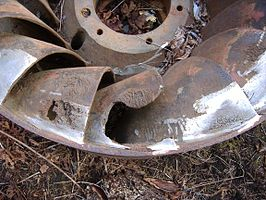
\includegraphics[width=0.7\columnwidth]{sota/figs/intro/cavitacao}
	\caption{Ilustração de uma pá de turbina que sofreu erosão por cavitação.}
	\label{fig::cavitacao}
\end{figure}

A fim de reduzir o desgaste da pá contra cavitação ou abrasão e aumentar a sua
vida útil, utiliza-se a técnica de revestimento por asperção térmica, que pode ser comparada com uma
tinta que protege à exposição com o ambiente. O procedimento é realizado
antes da instalação das pás na turbina por um robô, pois exige alta precisão
e velocidade, além de expelir substâncias nocivas à saúde. Apesar de suficiente para a proteção da pá, o
revestimento também tem vida útil e precisa ser refeito de tempos em tempos para
garantir a proteção da pá contra os fenômenos físicos.

No caso específico da usina hidrelétrica de Jirau, construída no rio Madeira,
os fenômenos de abrasão são intensos devido ao grande número
de partículas que o rio carrega diariamente, reduzindo ainda mais a vida útil do
revestimento.
Portanto, há a necessidade de manutenção regular, o que, na situação atual,
exige paralização da máquina, desmontagem da turbina, posicionamento de cada pá
na área designada ao revestimento, aplicação do revestimento, montagem da
turbina e recalibração. O tempo de paralização para a realização de
toda a manutenção pode levar de um a dois meses, significando uma grande perda
na geração de energia. 

A primeira etapa do projeto EMMA, pesquisa e desenvolvimento
realizados pela Fundação COPPETEC, em parceria com a empresa Rijeza, ANEEL e
ESBR, é um estudo de viabilidade técnica de um sistema robótico para realizar
revestimento por aspersão térmica de turbinas \textit{in situ}, ou seja, dentro
do ambiente da turbina (aro câmara). O projeto tem como objetivo reduzir
significativamente o tempo de manutenção do revestimento por ser realizado no
ambiente confinado da turbina e, portanto, não havendo necessidade de sua
desmontagem.

Este capítulo está dividido da seguinte forma: a seção 2 descreve
detalhadamente o problema, contextualiza o leitor no ambiente da usina de
Jirau e descreve as possíveis tarefas do robô; a seção 3 faz um levantamento do
estado da arte; a seção 4 descreve os projetos conceituais para o robô; e a
seção 5 conclui e descreve os próximos passos para o projeto EMMA. 



 
\section{Descrição do problema}\label{sec::consideracoes}

O fenômeno de cavitação e abrasão em hidroturbinas provoca desgaste
superficial por erosão e alteração do perfil
hidráulico da pá, gerando redução da eficiência na geração de energia.
Uma solução preventiva é o revestimento por metalização das pás, o qual aumenta a eficiência na
geração de energia por gerar uma estrutura mais lamelar, e fornece maior
resistência a desgastes. No caso da usina hidrelétrica de Jirau, o revestimento
das pás é realizado antes da montagem e instalação da turbina, porém devido ao grande número de
partículas e sedimentos que o rio madeira carrega e à cavitação, o revestimento
deve ser aplicado novamente em intervalos curtos de tempo
\citep{santa2009slurry}. A desmontagem da turbina, aplicação de novo
revestimento nas pás e remontagem são um processo muito custoso e deverá ser
feito regularmente. Portanto, há a necessidade de o procedimento ser
executado dentro do aro câmara, \textit{in situ}, onde as pás são instaladas.

A cavitação é a formação de cavidades de vapor (bolhas), em um líquido, devido a
quedas repentinas de pressão. Quando o líquido é sujeito ao aumento de pressão,
as bolhas implodem, ocasionando ondas de choque \citep{brennen2013cavitation}.

Em hidroturbinas, o fenômeno de cavitação é comum próximo às pás ou
na saída da turbina. O líquido apresenta a combinação
de componentes cinético, potencial gravitacional e energia de fluxo. O
componente cinético é em virtude do fluxo da água (velocidade), o potencial tem
relação com a altitude, e a energia de fluxo é energia que um fluido contém
devido à pressão que possui. De acordo com o princípio de Bernoulli, o princípio
da conservação para os fluidos, implica-se que, para uma mesma altitude, o
aumento da componente cinética acarreta em uma diminuição da pressão, ocorrendo
cavitação. 

Quando há cavitação, a formação de bolhas grandes altera as características do
escoamento, ocasionando oscilações ou vibrações na máquina que, por
conseqüência, prejudicam o rendimento do sistema hidráulico. As bolhas
pequenas, ao colapsar, geram ondas de choque de alta frequência, podendo provocar erosões se
próximo à superfície metálica.

Além da cavitação, como a água atravessa o aro câmara em grande velocidade, o
acúmulo de sedimentos irá provocar desgaste abrasivo, isto é, perda de material
pela passagem de párticulas rígidas. 

Nesta seção, são apresentadas as formas de reduzir os danos da cavitação pela
tecnologia de revestimento por metalização, a contextualização do problema no
caso da usina hidrelétrica de Jirau e as tarefas que um sistema robótico deve
realizar para solucionar o problema.


\subsection{Descrição do processo HVOF}\label{sec::desc_hvof}
O revestimento por aspersão térmica (ou metalização) é um processo em que
partículas aquecidas são pulverizadas em uma superfície a fim de melhorar ou
restaurar suas propriedades e dimensões. O revestimento estende a vida útil do
material, aumentando significantemente a sua resistência à erosão e corrosão.
Os diferentes tipos de metalização são: por chama, arco elétrico, detonação,
chama de alta velocidade (HVOF), plasma, a frio e a quente.

Um sistema de metalização é composto por: uma pistola de aspersão, responsável
pelo derretimento e aceleração das partículas a serem depositadas na
superfície; um alimentador, que fornece o pó (partículas) através de tubos;
um fornecedor do material de combustão; um robô para manipular a pistola; uma
fonte de alimentação elétrica para a pistola; um console de controle para o
sistema.

No caso específico das pás (aço inox 420) das turbinas da usina hidrelétrica de
Jirau, antes da montagem da turbina, a metalização tipo HVOF é realizada em
ambos os lados da pá pela empresa RIJEZA com um manipulador industrial de 150 kg
de carga máxima, permitindo controle de vibrações com boa margem de segurança, já que a massa do
sistema pode chegar a 10 kg (cabos e pistola). O tempo
mínimo do processo é de 6 horas por lado da pá.

O HVOF consiste em alimentar, numa câmara de combustão, o material de
revestimento (carboneto de tungstênio), uma mistura gasosa do combustível (propano) e
oxigênio. De acordo com os dados fornecidos pela empresa RIJEZA, a pistola de 8
Kg projeta uma chama de $3000^oC$, que pulveriza as partículas com velocidade de
700 a 1000 m/s, gerando uma força de recuo de 15 N.

O manipulador robótico deve possuir precisão de 5 mm, a pistola no efetuador
deve permanecer a uma distância que varia entre 230 e 240 mm, e ângulo de $90^o
\pm 60^o$, em relação à superfície. O manipulador deve ser capaz de
mover a pistola a velocidade constante de 40 m/min, e não pode permanecer uma
posição da pá por muito tempo (parada), pois há acúmulo de material, deformando a
superfície. Trocas de direção ou sentido na movimentação do manipulador são
considerados como parada, logo as trocas deverão ser realizadas em áreas
exteriores à superfície da pá ou chapas de sacrifício são utilizadas. 

Placas de sacrifício, ou mascaramento, são chapas colocadas em regões onde as
peça não podem ser jateadas ou revestidas. Geralmente uma chapa de qualquer tipo
de aço pode ser utilizada, pois a chama não fica parada sobre ela por um longo
período, não aquecendo-a o suficiente para danificar. Quando a pistola
permanece, em funcionamento, a chama é apontada para algum lugar onde não tenha obstáculos.

 % As informações do processo
% podem ser observadas na figura~\ref{fig::hvof}.
 
%\begin{figure}[h!]	
%	\includegraphics[width=\columnwidth]{sota/figs/intro/hvof.pdf}
%	\caption{Foto do efetuador do manipulador e pistola HVOF.}
%	\label{fig::hvof}
%\end{figure}

Em relação às condições de operação: o espaço da aplicação HVOF é confinado,
com excesso (100 a 140 dB), gases nocivos e com risco de explosão podem
ser exalados; a pá pode atingir temperaturas de até $110^oC$; as condições de
umidade e temperatura devem ser ideais para o processo; e há perda de $40\%$
das partículas pulverizadas  \citep{wu2006rebound}, que são espalhadas pelo
ambiente. Portanto, algumas medidas devem ser tomadas para a execução do
processo: a operação deve ser remota, não há presença de pessoas \textit{in
loco}; os gases presentes e umidade/temperatura devem ser constantemente
monitorados; o robô manipulador é selado; as partículas desperdiçadas devem
ser removidas (limpeza); e o desligamento do sistema deve ser acompanhado por corte de gás.

A qualidade do revestimento é geralmente avaliada por um instrumento que
realiza a medida de porosidade, oxidação, dureza e rugosidade da superfície. O
processo é realizado manualmente, de maneira rápida e fácil, por um operador.

A tabela~\ref{tab::hvof} resume as restrições e especificações do
projeto:

\begin{center}
\begin{tabular}{  c | c  }
  \hline
  \textbf{Componente} & \textbf{Dado} \\ \hline
  Massa da pistola HVOF & 8 Kg  \\ \hline
  Massa dos cabos HVOF & 12 Kg  \\ \hline
  Tempo HVOF por pá & 6 horas \\ \hline
  Temperatura da chama HVOF & $3000^oC$ \\ \hline
  Recuo da pistola & 15 N \\ \hline
  Precisão do manipulador & 5 mm \\ \hline
  Distância pistola-pá & 230-240 mm \\ \hline
  Ângulo pistola-pá & $30^o$-$90^o$ \\ \hline
  Velocidade do manipulador & 40 m/s \\ \hline
  Ruído HVOF & 100 a 140 dB \\ \hline
  Temperatura da pá & $110^oC$ \\
  \hline
\end{tabular}
\captionof{table}{Dados principais do processo HVOF}
%\caption{Dados principais do processo de metalização HVOF}
\label{tab::hvof}
\end{center}

%Sistemas robóticos não devem utilizar magnetismo como meio de aderência, já que
%o aço inox 420 não apresenta alta permeabilidade magnética e a alta temperatura
%da pá deve inviabilizar essa solução. Adesão por ventosas é uma solução
%viável, pois material não causa dano ao revestimento, porém a escolha do
%material da ventosa deve ser estudado,já que a pá quente pode ocasionar em
%perda de sucção, como em ventosas emborrachadas.


\subsection{Descrição dos requistios de operação de HVOF}

O processo de metalização de turbinas hidrelétricas tem alguns pré-requisitos
que devem ser respeitados para uma correta aplicação e fixação da camada de
material durante o revestimento. Essa subseção descreverá as etapas necessárias
de preparação da superfície a fim de se assegurar a manutenção da qualidade dos resultados e do
perfil hidráulico da pá. 

\subsubsection{Jateamento da superfície da pá}\label{sec:jat}

O processo de metalização sobreposto a uma superfície que já possui uma camada
protetora desgastada não apresenta um resultado tão satisfatório se comparado
com o processo realizado em uma superfície crua. Por esse motivo é recomendado
que seja realizado um processo de jateamento abrasivo. 

O jateamento consiste em direcionar um fluxo de material abrasivo na superfície
do material a fim de se erodir a mesma e retirar o material depositado na camada
superficial. Outra característica desse processo é a capacidade de aumentar a
rugosidade da superfície e, assim, aumentar o poder de adesão da nova camada a
ser metalizada.  

O processo de jateamento para o tratamento específico da superfície das pás da
turbina utiliza óxido de alumínio como material abrasivo e pode ser realizado
por um operador. A infraestrutura necessária para esse processo é uma fonte de
ar comprimido, geralmente proveniente de um compressor de ar, para propulsionar
o particulado que forma o jato abrasivo. %\textbf{A preparação do ambiente no
% envolto da pá, o escoamento do material e
%as consequências da realização desse processo não foram analisados} e,
%possivelmente, será necessária a implementação de infraestrutura de suporte
%para proteção dos equipamentos adjacentes que não receberão o jateamento,
%limpeza do material depositado e exaustão do particulado suspenso.

\subsubsection{Reparo de danos existentes}

Danos existentes na superfície da pá ou em sua estrutura podem reduzir a sua
eficiência e até mesmo a própria integridade da pá, prejudicando a segurança 
da operação. O processo de metalização não tem a capacidade de reparar
danos severos na superfície ou danos estruturais como rachaduras. A inspeção
para procura desses defeitos deve ser realizada antes da realização do processo
de metalização, uma vez que a superfície jateada, ou seja, em metal cru sem
camada de proteção, facilita a visualização de danos. %Os procedimentos para
%reparos de danos estruturais ou referentes a rachaduras não serão cobertos por
%este documento.

Os danos causado por cavitação, como explicado na seção
\ref{sec::consideracoes}, pode alterar o perfil hidráulico da pá e deve ser
reparado sempre que possível. O procedimento de reparo varia de acordo com a
severidade dos danos causados. À medida que a profundidade das cavidades geradas
na pá e a extensão dos danos vão aumentando, medidas mais extremas se tornam
necessárias e, por isso, a estratégia de reparo para esse tipo de dano deve
estar alinhada com o tipo de processo que se deseja utilizar. Inspeções e
reparos mais frequentes significam processos mais simples, enquanto que reparos
mais espaçados podem resultar até na inutilização da pá. Os procedimentos mais
utilizados para o reparo de danos causados por cavitação são:

\begin{itemize}
  \item Reparo com materiais não fundidos à superficie;
  \item Reparo por solda;
  \item Reparo por solda e placa sólida.
\end{itemize}

\paragraph{Reparo com materiais não fundidos à superficie}
Para pequenos danos, é possível utilizar processos nos quais não é necessário
fundir o material depositado para preenchimentos das cavidades ao material da
superfície metálica da pá. Os processos e materiais utilizados, usualmente na
indústria, são: 

\begin{itemize}
\item Epoxy;
\item Cerâmica;
\item Revestimento por metalização;
\item Neoprene;
\item Urethane.
\end{itemize}

Vale ressaltar que a solução proposta para a metalização de uma camada protetora
para se evitar os danos causados pela cavitação também poderia ser utilizado
para preencher danos passados, desde que respeitem o limite de espessura
para o tipo de processo utilizado


\paragraph{Reparo por solda}

O preenchimento dos danos causados devido à cavitação por solda é o procedimento
mais comum, pois possibilita uma maior deposição de material e não obriga a
realização de reparos com uma frequência elevada. Esse processo consiste na
deposição de solda em camadas, até o completo preenchimento. A
superfície deve ser, então, esmerilhada até entrar em conformidade com as
medidas padrão de qualidade para o perfil hidráulico da pá a ser reparada. Essa tarefa
é normalmente realizada por mão de obra altamente qualificada e existe, também,
na literatura a presença de soluções automatizadas, como os robôs Roboturb e Scompi
\citep{roboturb,scompi}

\paragraph{Reparo por solda e placa sólida}

Para casos de danos mais severos, pode ser necessária a utilização de placas
para o preenchimento de grandes extensões. O processo de fixação das placas é
realizado por solda, assim como o preenchimento do volume restante. O processo
de solda, esmerilhamento e verificação é comum ao procedimento padrão utilizando
somente solda.
















\subsection{Contextualização do Ambiente}\label{sec::desc_contex}

A usina hidrelétrica Jirau é do tipo fio d'água, na qual são utilizadas turbinas
do tipo bulbo de eixo horizontal. Como a geração de energia depende da altura da queda d'água e da vazão do rio, as turbinas do tipo bulbo utilizam uma grande vazão de
água para produzirem energia elétrica suficiente. A figura
\ref{fig::bulb_turbine} e a tabela \ref{tab::bulb_turbine} ilustram uma turbina
do tipo bulbo e o grandes dutos necessários para comportar o grande volume de água que passa através da turbina. 
 
\begin{figure}[h!]	
	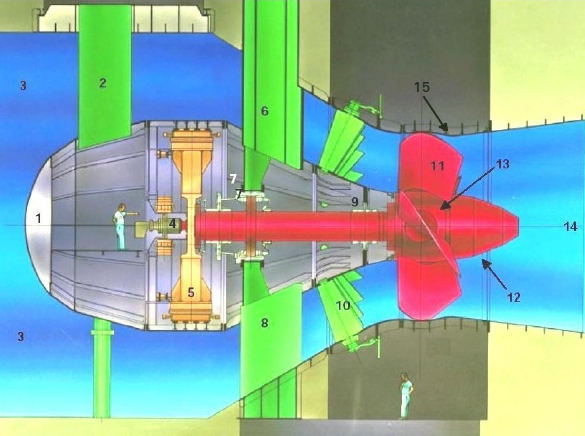
\includegraphics[width=\columnwidth]{sota/figs/intro/bulb_turbine2}
	\caption{Ilustração de uma turbina do tipo bulbo.}
	\label{fig::bulb_turbine}
\end{figure}

\begin{center}
\begin{tabular}{  c | c  }
  \hline
  \textbf{Número} & \textbf{Componente} \\ \hline
  1 & Nariz do bulbo \\ \hline
  2 & Tubo de acesso ao gerador  \\ \hline
  3 & Câmara de adução  \\ \hline
  4 & Cabeçote Kaplan  \\ \hline
  5 & Gerador Síncrono  \\ \hline
  6 e 8 & Estrutura de sustentação \\ \hline
  6 & Tubo de acesso à turbina \\ \hline
  7 e 9 & Mancais Combinado e Guia \\ \hline
  10 & Distribuidor \\ \hline
  11 & Pás do Rotor \\ \hline
  12 & Cone ou Ogiva \\ \hline
  13 & Cubo \\ \hline
  14 & Tubo de sucção/descarga \\ \hline
  15 & Aro Câmara \\
  \hline
\end{tabular}
\captionof{table}{Componentes principais de uma turbina tipo bulbo}
%\caption{Componentes principais de uma turbina tipo bulbo}
\label{tab::bulb_turbine}
\end{center}



Atualmente, caso seja necessário algum reparo ou inspeção na turbina, é necessário que se interrompa o fluxo de água e que 
toda a água em seu interior seja drenada. Para manutenção do rotor, existe uma escotilha de acesso de diâmetro limitado. Entretanto, caso deseje-se realizar 
a metalização de pás já instaladas, utilizando-se os processos atuais, é
necessária a retirada de todo o aro câmara, desmontagem completa do rotor e logística de transporte das pás até o local
onde a metalização será realizada. Essa operação, caso necessite ser realizada, demandaria a mobilização
de diversas equipes de manutenção, operação de pórtico rolante e transporte,
além de impossibilitar a utilização da turbina durante várias semanas.
No contexto da solução proposta, os pontos de interesse da turbina são:

\begin{itemize}
  \item Hélice e pás;
  \item Aro Câmara e regiões adjacentes;
  \item Escotilhas de acesso;
  \item Tubo de Sucção;
  \item Infraestrutura disponível
\end{itemize} 

\subsubsection{Hélice e pás}
 
O rotor ou hélice da turbina é constituído do cubo, as pás e o cone. 
Nas turbinas da usina Jirau, cada pá mede, aproximadamente, 2,5m de altura e
3m de largura. A partir do interior da turbina, todas as superfícies da pá são
alcançáveis, com exceção da borda e do lip da pá. O único ponto de acesso à
essa regiâo é por meio da escotilha superior de acesso. A figura
\ref{fig::blade_rijeza} exemplifica uma pá do rotor presente na usina Jirau recém metalizada no galpão da Rijeza.

\begin{figure}[h!]
	\centering	
	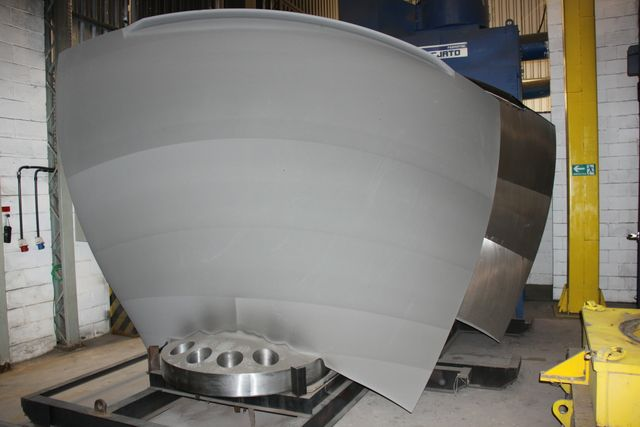
\includegraphics[width=0.7\columnwidth]{sota/figs/viagem/img_4887}
	\caption{Pá do rotor recém metalizada.}
	\label{fig::blade_rijeza}
\end{figure}

A angulação de cada pá em relação ao fluxo d'água pode ser alterado em 29$^o$,
14.5$^o$ para cada lado a partir da posição inicial, não havendo sobreposição
entre as pás, como ilustrado na figura \ref{fig::blades_angle}.
Essa angulação pode ser explorada para otimizar o espaço de trabalho necessário
para o processamento da pá e também influencia o acesso à região
entre o distribuidor e o rotor, uma vez que não existe acesso pela montante da
turbina. Entretanto, vale observar que esta angulação não pode ser alterada
manualmente e só pode ser realizada uma vez, antes do desligamento da turbina. A
posição do rotor também pode ser manualmente alterada, possibilitando que o mesmo seja girado em ambas as direções e sem limite de revoluções. Entretanto, essa operação é uma tarefa imprecisa e envolve um certo risco às pessoas que a realizam. Sendo
assim, a solução proposta deve otimizar o número de rotações necessárias para o processamento de todas as pás.

\begin{figure}[h!]	
	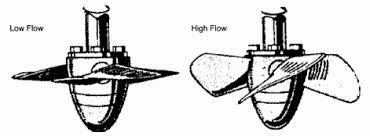
\includegraphics[width=\columnwidth]{sota/figs/intro/blades_angle}
	\caption{Exemplo de limites de rotação das pás do rotor.}
	\label{fig::blades_angle}
\end{figure}

\subsubsection{Aro Câmara e regiões adjacentes}

O aro câmara, assim como o a região próxima ao distribuidor e também ao tubo de
sucção possuem superfícies metálicas. Essa característica possibilita a
exploração de soluções de fixação magnética.

Somente a região compreendida pelo aro câmara é plana e tendo como agravante a presença do distribuidor na região à 
montante ao rotor. É necessário que a inclinação presente nessas superfícies seja contabilizada e uma solução eficiente 
de apoio ou plano elevado seja desenvolvida caso haja necessidade de fixação de alguma parte do sistema. Atualmente todo 
o trabalho é realizado por meio da montagem de andaimes ancorados por cordas. %A
%figura \ref{fig::andaime} ilustra uma estrutura utilizada no modo de inspeção e
%manutenção atuais.

%\begin{figure}[h!]	
%	\centering
%	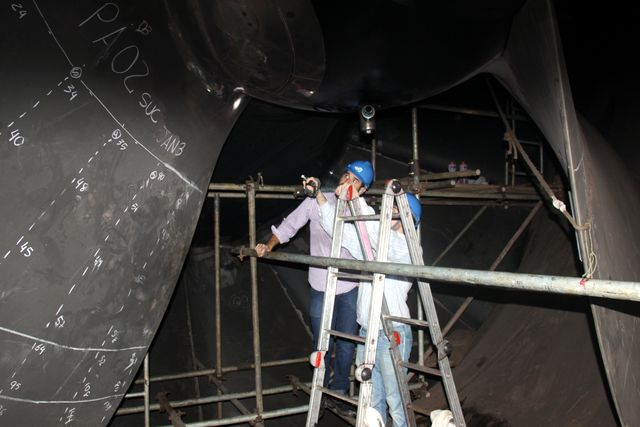
\includegraphics[width=0.8\columnwidth]{sota/figs/viagem/img_4969}
%	\caption{Andaime montado no interior da turbina e ancorado por cordas}
%	\label{fig::andaime}
%\end{figure}

 
\subsubsection{Escotilhas de acesso}
O acesso à turbina se dá por duas escotilhas, uma inferior, localizada no ínicio do tubo de sucção 
próxima ao aro câmara e outra superior, localizada na parte superior do aro câmara.

A escotilha inferior, ilustrada na figura \ref{fig::esc_inf} é o acesso
utilizado para a entrada de pessoas na turbina e todo material utilizado para reparos é transportado através dessa escotilha. Na usina Jirau existem dois 
tipos de escotilha de acesso inferior, sendo a menor delas possuindo 80cm de diâmetro. 

A escotilha superior é utilizada, principalmente, para a inspeção visual do
estado dos Lips das pás.
O diâmetro do acesso superior é de aproximadamente $35.7cm$, limitando as
dimensões dos equipamentos que podem ser transportados através da escotilha. As figuras \ref{fig::esc_sup_ext} e
\ref{fig::esc_sup_int} ilustram o acesso à escotilha superior pelo exterior ao
aro câmara e a visão pelo interior da turbina,
respectivamente.

\begin{figure}[h!]	
	\centering
	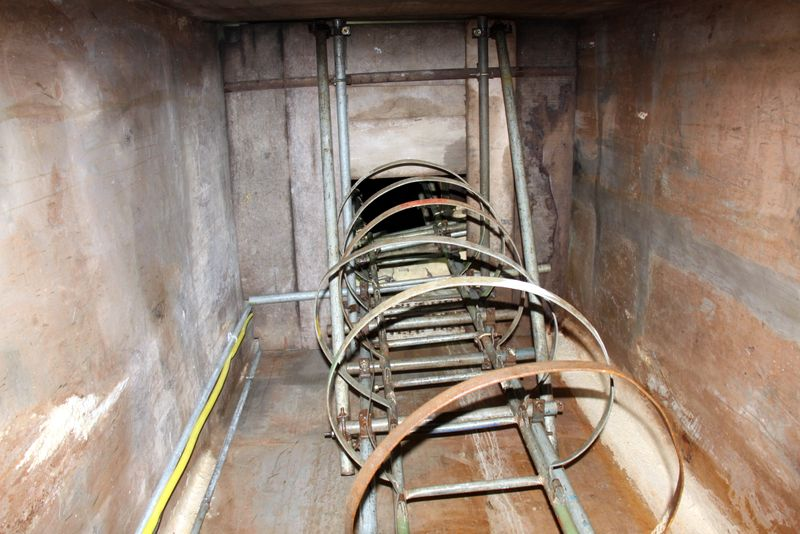
\includegraphics[width=0.8\columnwidth]{figs/esc_inf}
	\caption{Vista exterior da escotilha inferior.}
	\label{fig::esc_inf}
\end{figure}




\begin{figure}[h!]	
	\centering
	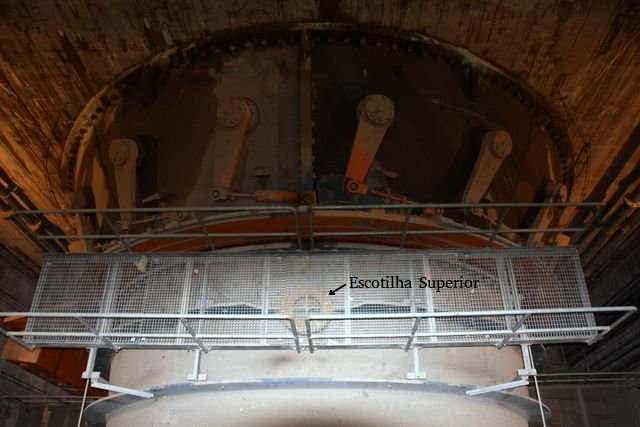
\includegraphics[width=0.8\columnwidth]{sota/figs/viagem/img_4979_mod}
	\caption{Vista da escotilha superior pelo exterior do aro câmara}
	\label{fig::esc_sup_ext}
\end{figure}

\begin{figure}[h!]	
	\centering
	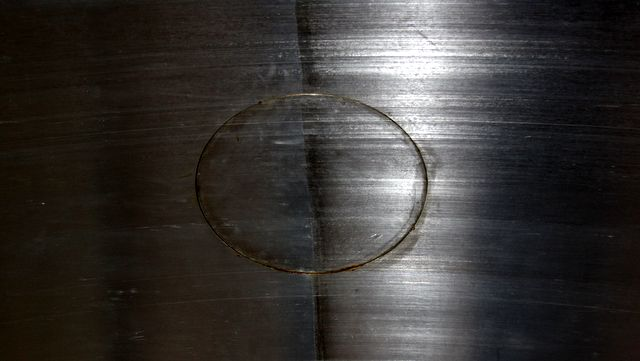
\includegraphics[width=0.8\columnwidth]{sota/figs/viagem/img_4982}
	\caption{Vista da escotilha superior pelo interior do aro câmara}
	\label{fig::esc_sup_int}
\end{figure}

\subsubsection{Tubo de sucção}

Ao final do tubo de descarga está localizado o vão dos stoplogs 
de jusante ou da comporta vagão e, em seguida, o leito do rio, como ilustrado
na figura \ref{fig::tubo_suc}.
Caso os stoplogs não estejam inseridos, existe um vão de, pelo menos, 10 m de largura. Porém, não
é válida a utilização deste vão como acesso à turbina, pois há grande fluxo de
água devido à abertura do distribuidor. O distribuidor não é fechado
imediatamente por questões ambientais, já que este é o escoamento de peixes.

%criando assim
%um acesso extra para um sistema submarino. A figura \ref{fig::tubo_suc}
%exemplifica a magnitude do tamanho do acesso, deixando claro que o limitante de
%tamanho do sistema para a utilização desse acesso é o vão de entrada do
% stoplog, ilustrado na figura \ref{fig::stoplog}. Outra alternativa é utilizar um
%guindaste e submergir o sistema pelo próprio rio, entretanto o sistema ficaria
%sujeito as condições do ambiente.

\begin{figure}[H]
	\centering	
	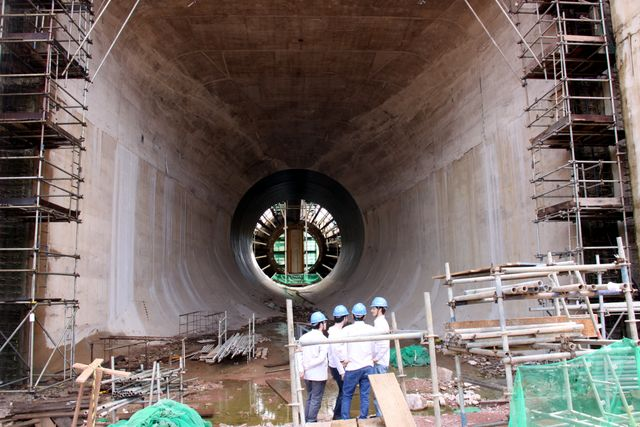
\includegraphics[width=0.8\columnwidth]{sota/figs/viagem/img_5086}
	\caption{Abertura do tubo de sucção para o leito do rio, em fase de
	construção.}
	\label{fig::tubo_suc}
\end{figure}

\subsubsection{Infraestrutura disponível}
É importante ressaltar a infraestrutura dísponível para o desenvolvimento da solução. 
Após o ensecamento da turbina, é possível a disponibilização de energia elétrica
e ar comprimo em seu interior, ambos importantes para o processo de metalização. Outro fator 
importante é a presença de um pórtico rolante que tem acesso até o andar diretamente 
inferior ao aro câmara, posicionando todo o equipamento necessário nas proximidades 
da escotilha de acesso inferior. É possível também o acesso direto, por meio de pórtico, 
à escotilha superior.

\begin{figure}[h!]	
	\centering
	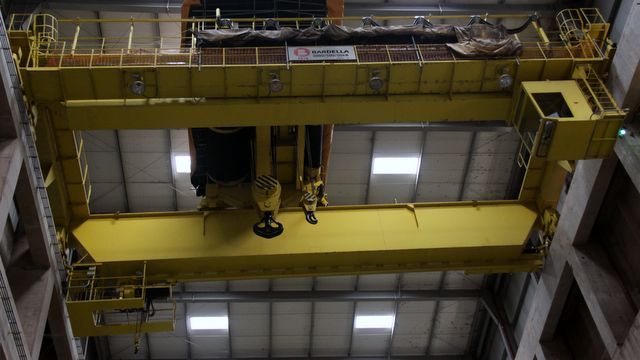
\includegraphics[width=0.8\columnwidth]{sota/figs/viagem/img_4989}
	\caption{Pórtico rolante com acesso ao exterior do aro câmara}
	\label{fig::portico}
\end{figure}


O ambiente pode ser resumidamente caracterizado pelas dimensões das pás,
elemento a ser processado; características do aro câmara, estrutura que limita o
espaço de trabalho do robô; e pelos acessos nos quais o sistema terá que
utilizar:

\begin{itemize}
  \item \textbf{Pás do rotor} - Material aço inox 420. Dimensões 2.5 x 2.5 m de superfície;
  \item \textbf{Aro Câmara} - estrutura cilíndrica com raio de 3.95 m e
  superfície metálica;
  \item \textbf{Acessos}: 
  	\begin{itemize}
    	\item Escotilha superior - 35 cm de diâmetro;
  		\item Escotilha inferior - 80 cm de diâmetro;
  		\item Tubo de descarga - 20 x 20 m, porém acessado pelo rio. 
  	\end{itemize}
\end{itemize}







\subsection{Descrição das tarefas do robô}
\label{desc_taref}
Esta subseção descreve as tarefas básicas do robô para o revestimento de
turbinas \textit{in situ}. Em linhas gerais, o robô a ser desenvolvido deve ser
capaz de realizar a tarefa de revestimento tal qual seria feita caso a pá não estivesse instalada na
tubina e de uma maneira autônoma. A pá, antes de ser submetida ao
processo de revestimento, deve estar em conformidade com o gabarito, perfil hidráulico de uma pá
intacta. Portanto, uma tarefa do robô é realizar o mapeamento do perfil
hidráulico, construir um modelo 3D e analisar imperfeições.

Em caso de deformações, causados por cavitação e abrasão, estas precisam
ser removidas manualmente ou de forma automatizada, possivelmente por
soldagem. A tarefa de soldagem pode
ser realizada por operador, manualmente, por não possuir todas as restrições
da tarefa de revestimento (velocidade, precisão, carga e etc), porém o ambiente
pode dificultar a operação de forma que a execução por um robô seja
indispensável. 

Após as pás estarem de acordo com o gabarito, faz-se a
identificação do desgaste do revestimento, medindo sua espessura em pontos
pontos específicos sobre a superfície da pá. Manualmente esse
processo é realizado eficientemente em 10 min, justificando a não necessidade de
esta ser uma tarefa do robô. 

Em caso de necessidade de aplicação
de novo revestimento, é necessária a remoção do revestimento antigo por
jateamento, a fim de deixar a superfície rugosa e aumentar sua aderência. A
tarefa de jateamento é atualmente realizada maualmente, mas também pode ser
realizada pelo robô. Como ambos os lados da pá são revestidos, o jateamento deve
ser realizado em ambos os lados. Vale ressaltar que, em teoria, pode-se aplicar revestimento por metalização sem retirar o último revestimento,
porém esse processo ainda se encontra em fase de estudos na Rijeza.
%Segue-se o exemplo de empresas de aviação, onde existe a
%prática de retirar todo o revestimento antigo antes de aplicar o novo.

Por fim, o robô deverá aplicar o revestimento como
forma de prevenir o dano causado pelos fenômenos abrasivos. O robô projetado
para fazer o revestimento precisa preencher todos os requisitos discutidos na
subseção~\ref{sec::desc_hvof} e ser adaptável ao ambiente, cujos as restrições
são discutidos na subseção~\ref{sec::desc_contex}. 

Das tarefas a serem relizadas, são destacadas as seguintes:

\textbf{Tarefas que podem ser executadas manualmente:}
\begin{itemize}
  \item Inspeção e análise de danos na pá, tanto para reparo quanto para
  revestimento;
  \item Reparo;
  \item Montagem do sistema;
  \item Jateamento da superfície;
\end{itemize}

\textbf{Tarefas que poderão ser executadas pelo robô:}
\begin{itemize}
  \item Modelar o perfil hidráulico;
  \item Calibração;
  \item Jateamento;
  \item Reparo (soldagem e esmerilhamento);
  \item Revestimento por metalização;
\end{itemize}




\section{Estado da arte}\label{sota/sota}
 
O estudo do estado da arte de robôs para a realização de HVOF em pás de turbinas
hidráulicas contempla os sistemas que atendem a alguns dos requisitos: operar
em ambientes de alta periculosidade; capacidade de carga para os dispositivos HVOF;
manipular a pistola HVOF com velocidade de $0.67 m/s$; precisão de 5mm; ter
área de trabalho de 2.5 m x 2.5 m; e operar sob superfícies 3D de geometria
complexa. As soluções foram divididas em subseções de acordo com as tecnologias
de fixação dos robôs.


 
\subsection{Robôs sobre trilhos}
\label{sec::rail}
Na indústria, a automatização de processos de metalização, é
normalmente realizada com a utilização de manipuladores robóticos, pois oferece
a versatilidade de tarefas e espaço de trabalho necessários para esse
tipo de aplicação. Entretanto, um sistema composto por um braço robótico capaz
de operar em toda a extensão da superfície da pá da turbina hidrelétrica
não é compacto, nem móvel o suficiente para ser instalado e desinstalado para a
operação de manuntenção \textit{in-situ}.

A introdução de uma junta prismática acoplada a um trilho é uma estratégia para
reduzir o tamanho e o peso de um manipulador robótico.  Assim, é possível estender o
 espaço de trabalho do robô, sem adicionar peso ao manipulador, uma vez que o
 trilho pode usar as estruturas presentes no ambiente como apoio. 

Na literatura foram encontradas duas soluções para aplicações de manutenção e
inspeção, como solda, específicas para o contexto de turbinas hidráulicas. As
aplicações diferem, principalmente, na estratégia de fixação do sistema
de trilhos.
O Roboturb \citep{roboturb} realiza a fixação
diretamente na pá do rotor, enquanto o robô Scompi \citep{scompi} utiliza um
trilho fixado em
estruturas adjacentes à pá ou peça a ser reparada.

O Roborturb consiste em um manipulador robótico com seis juntas de revolução e
uma junta primsática acoplada a um trilho flexível, como pode ser observado
na figura \ref{fig::roboturb}, utilizado para o preenchimento de cavidades
geradas por cavitação.
O trilho pode ser conformado e, então, fixado à superfície da pá por meio de um
 sistema passivo de ventosas ou ímãs. O robô tem a possibilidade de utilizar dois 
 efetuadores distintos, o primeiro consiste em um sensor ótico para inspeção do 
 estado de erosão da pá e o segundo consiste em uma ferramenta de solda do 
tipo tocha plasma PWH-4A com alimentador automático de arame, responsável pelo 
depósito de solda para o preenchimento das cavidades identificadas pelo sistema.


%TODO Abelha: Posicionar corretamente as figuras
    \begin{figure}[h!]	
		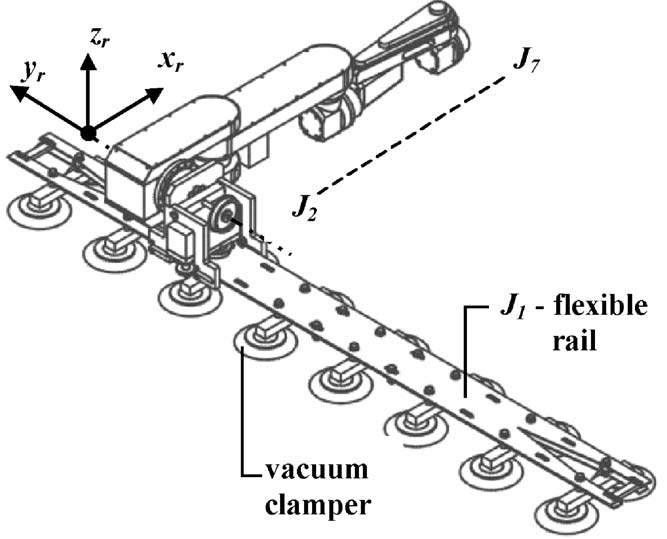
\includegraphics[width=\columnwidth]{sota/figs/trilhos/roboturbpaper}
		\caption{Roboturb - Manipulador robótico sobre trilho flexível}
		\label{fig::roboturb}
	\end{figure}
	\begin{figure}[h!]
		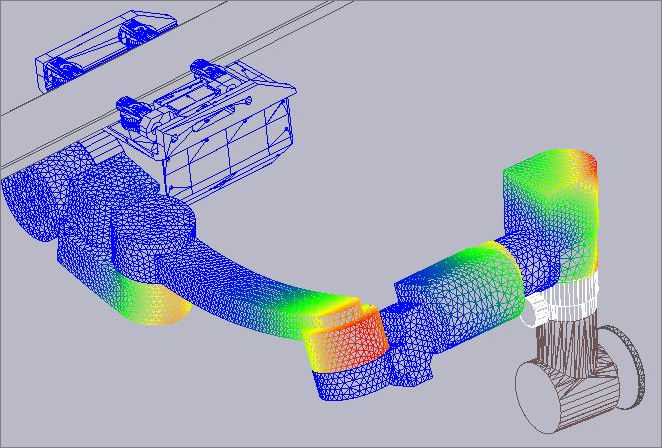
\includegraphics[width=\columnwidth]{sota/figs/trilhos/scompi}
		\caption{SCOMPI - Manipulador robótico sobre trilhos rígidos}
		\label{fig::scompi}
	\end{figure}

Por sua vez, o robô Scompi, fig \ref{fig::scompi}, é um manipulador
multipropósito projetado para realizar reparos em turbinas do tipo \textit{Francis},
 como solda e esmerilhamento das pás. O sistema possui seis graus de liberdade,
 sendo consitituído por um braço robótico com cinco juntas de revolução, e o
 último grau de liberdade proveniente de uma junta prismática que percorre um sistema de 
 trilhos retos ou curvos que são projetados para cada aplicação especificamente. 


Sistemas baseados em trilhos tem como maior benefício a redução do tamanho e,
consequentemente, do peso do manipulador necessário para a execução de tarefas
em um espaço de trabalho que englobe toda a superfície da pá.
Essa redução proporciona facilidade de transporte do robô até o interior da
turbina e também possibilita o projeto de manipuladores que tenham a rigidez
necessária para a realização das tarefas desejadas. 

Manipuladores robótico fixos, rígidos o suficiente para aguentar as forças intrínsecas ao
processo de metalização e com espaço de trabalho necessário para trabalhar em
toda a extensão da superfćie da pá seriam muito pesados.
Entretanto, sistemas baseados em trilhos com fixação na própria pá do rotor, necessitam que
o trilho seja movido caso se deseje que toda a superfície da pá sofra
manuntenção, uma vez que a área em que o trilho está apoiado não pertence ao espaço de
trabalho do robô. Em adição, sistemas com fixação de trilhos nas estruturas
adjacentes à pá devem atentar as condições para a instalação disposta pelo
ambiente para equilibrar a relação de custo benefício entre facilidade de
instalação/remoção do trilho e a robustez.

\textbf{Vantagens:}
\begin{itemize}
  \item Redução do tamanho necessário do manipulador;
  \item Redução do peso do manipulador
\end{itemize}

\textbf{Desvantagens:}
\begin{itemize}
  \item Necessidade de instalação e remoção dos trilhos;
  \item Necessidade de movimentação dos trilhos (para trilhos fixados
  diretamente nas pás)
\end{itemize}



 
\subsection{Robôs escaladores}\label{sota_climbers}
Robôs escaladores são sistemas capazes de sustentar seu próprio peso contra a
gravidade, movendo-se em simples ou complexas estruturas geométricas, como
paredes, tetos e telhados, palhetas de turbinas e plantas nucleares.
Essa classe de robôs oferece eficiência operacional em ambientes
de alta periculosidade, sendo utilizados visando saúde e segurança dos
trabalhadores, como em inspeção e limpeza de arranha-céus, diagnóstico de
tanques de armazenamento em plantas nucleares, solda e manutenção de cascos de
navios e palhetas de turbinas \citep{armada2003application}. 

Os grandes desafios nos projetos de sistemas escaladores são mobilidade e
aderência, além de consumo de energia, capacidade de carga e peso. Em
\cite{modular} e \cite{climbsurv}, os robôs escaladores são divididos em tipos
de locomoção:
pernas; como andador; utilizando segmentos deslizantes; rodas; esteiras; avanço
pendurado por braços; por cabos; e biomimética. E categorias de adesão: sucção
ou pneumática; magnética; eletrostática; química; preensão; e híbrida.

No caso específico deste estudo da arte, destacam-se os robôs escaladores com as
seguintes aplicações:

\begin{itemize}
  \item \emph{Navios e turbinas}: RRX3 para soldagem
  \citep{rrx3}, \emph{Climbing Robot for Grit Blasting} para limpeza
  \citep{crgb} e ICM Robot para inspeção \citep{icm};
  \item \emph{Industrial}: ROMA II \citep{roma} e
  CROMSCI \citep{CROMSCI}, ambos para inspeção; 
 \item \emph{Planta petroquímica}: TRIPILLAR \citep{tripillar} para inspeção.  
\end{itemize}

O RRX3 (figura~\ref{rrx3}), Daewoo Shipbuilding and Marine Engineering, é um
robô para a soldagem de casco de navios. Possui adesão por preensão, locomoção transversal utilizando segmentos deslizantes e locomoção
longitudinal por rodas. Possui um manipulador de 1.5 m com três juntas
prismáticas e três juntas de revolução (3P3R) para a operação de soldagem. 

As características principais do robô são: base e manipulador com
capacidades de carga de 120 kg e 5 kg, respectivamente; manipulador com precisão
milimétrica e efetuador de baixa velocidade; robustez para operar em ambiente de
alta periculosidade; opera instrumento de solda; e locomoção transversal é
restrita à aplicação.

\begin{figure}[ht]
\centering
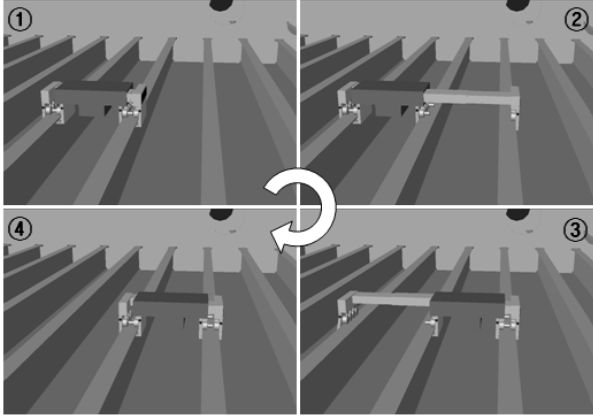
\includegraphics[width=\columnwidth]{sota/figs/climbers/RRX3_moving.jpg}
\caption{Translação horizontal do robô RRX3.}
\label{rrx3}
\end{figure}

O \emph{Climbing robot for Grit Blasting} (figura~\ref{grit}), University of
Coruna, é um robô para jateamento abrasivo em navios. O robô utiliza duas plataformas deslizantes com sistema de adesão por
ímã magnético. Os módulos apresentam movimentação relativa entre si e pode rotar
para compensar as curvaturas do casco do navio ou desviar de objetos. 

As características principais do robô são: base com
capacidade de carga de sistema abrasivo semelhante a HVOF; base com
locomoção de precisão milimétrica; locomoção ampla, mas não aplicável a
estruturas complexas; e não possui manipulador, sendo necessário percorrer todo
o casco.

\begin{figure}[ht]
\centering
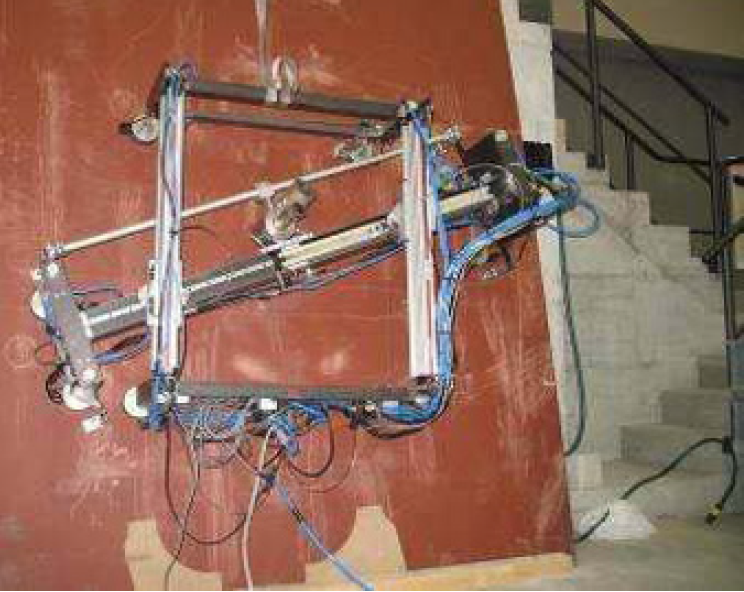
\includegraphics[width=\columnwidth]{sota/figs/climbers/grit.png}
\caption{Climbing robot for Grit Blasting}
\label{grit}
\end{figure}

\emph{The Climber} (figura~\ref{icm}), ICM Robotics, é um robô para inspeção de
turbinas eólicas, remoção de revestimento, limpeza de superfície, e aplicação de revestimento.
Possui adesão pneumática (sucção) e locomoção por esteiras. 

As características principais do robô são: base com capacidade de carga de 25
kg; base com locomoção de precisão milimétrica; manipulador modular pode ser
acoplado à base; manipulador de dimensão reduzida e baixa velocidade; e
locomoção apresenta restrição a algumas curvaturas acentuadas.

\begin{figure}[ht]
\centering
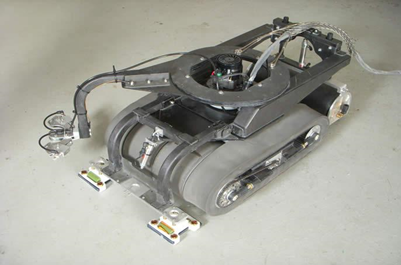
\includegraphics[width=\columnwidth]{sota/figs/climbers/icm.png}
\caption{Robô The Climber da ICM Robotics}
\label{icm}
\end{figure}

O ROMA II (figura~\ref{roma2}), Universidade Carlos II de Madrid, é um robô para
inspeção de ambientes complexos. A sua tecnologia de adesão é pneumática (sucção) e
locomove-se como uma lagarta (biomimética). Sua movimentação e planejamento de
trajetória são realizados de maneira ótima de forma a garantir estabilidade e
evitar obstáculos. 

As características principais do robô são: base com grande capacidade de carga;
base com locomoção de precisão milimétrica; não possui manipulador; locomoção em
ambientes de grande complexidade.

\begin{figure}[ht]
\centering
%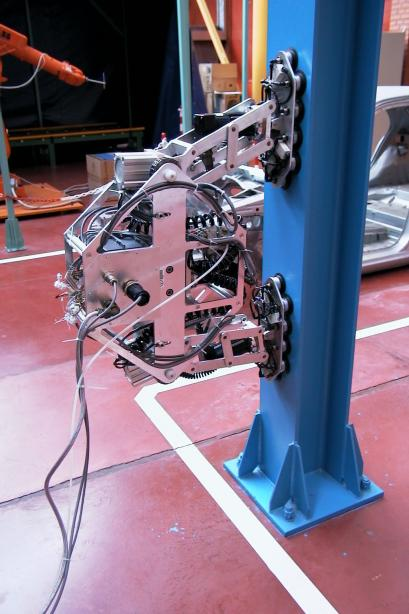
\includegraphics[width=8.4cm]{sota/figs/climbers/roma2.jpg}
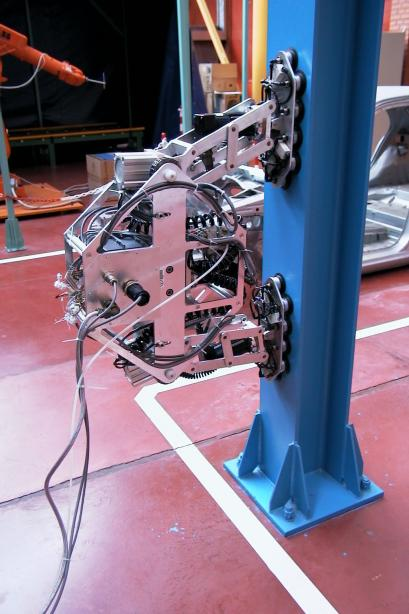
\includegraphics[width=\columnwidth]{sota/figs/climbers/roma2.jpg}
\caption{ROMA II.}
\label{roma2}
\end{figure}

CROMSCI (figura~\ref{cromsci}), Kaiserslautern University of Technology, é um
robô autônomo para inspeção de grandes paredes de concreto, como pilares de pontes, barragens. Seu
sistema de adesão é composto por sete câmaras de vácuo (sucção), com um sistema
de controle por válvulas e sensores de pressão para reagir rapidamaente a
condições adversas. Locomove-se com rodas omnidirecionais para locomoção.

As características principais do robô são: base com pouca capacidade de
carga; base com locomoção de precisão milimétrica; não possui manipulador; e
apresenta baixa velocidade.

\begin{figure}[ht]
\centering
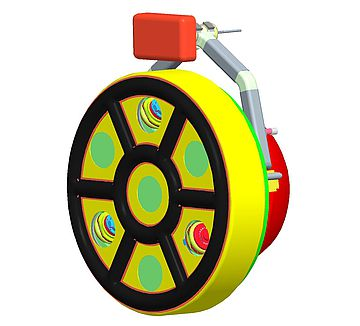
\includegraphics[width=\columnwidth]{sota/figs/climbers/cromsci.jpg}
\caption{Robô CROMSCI.}
\label{cromsci}
\end{figure}

TRIPILLAR (figura~\ref{tripillar}), École polytechnique fédérale de Lausanne, é
um robô escalador de pequeno porte (96 x 46 x 64 mm) desenvolvido para a inspeção de plantas
petroquímicas. Utiliza um sistema como pernas de lagarta magnéticas em um
formato triangular. Locomove-se por esteiras.

As características principais do robô são: base com pouca capacidade de
carga; base com locomoção de precisão milimétrica; sistema robusto a aplicações
em ambientes de alta periculosidade; sistema de controle simples; robô de
pequenas dimensões; não possui manipulador; sistema ainda não testado em estruturas geométricas complexas.


\begin{figure}[ht]
\centering
\includegraphics[width=\columnwidth]{sota/figs/climbers/tripillar.png}
\caption{Robô TRIPILLAR.}
\label{tripillar}
\end{figure}
   
Os robôs escaladores são utilizados em diversas aplicações e possuem diferentes
soluções de aderência e locomoção, como foi exposto nesta subseção. Não há,
até o momento, um robô escalador que possui todas as características
exigidas para a tarefa de HVOF em pás de turbinas, porém a adaptação de
alguns desses sistemas, como \emph{The Climber} da ICM Robotic, pode gerar
soluções completas.

As vantagens e desvantagens para solução de robôs escaladores são:

\textbf{Vantagens:}
\begin{itemize}
  \item Facilidade de instalação;
  \item Manipulador de pequenas dimensões, já que o robô se movimenta sob a pá
  da turbina;
  \item Base de pequenas dimensões;
  \item Pouco peso;
  \item Autonomia durante a operação em uma pá; 
\end{itemize}

\textbf{Desvantagens:}
\begin{itemize}
  \item Sistema de locomoção complexo com desvio de obstáculo e planejamento de
  trajetória;
  \item Desafio mecânico na construção de uma estrutura capaz de sustentar seu
  peso mais o manipulador com sistema HVOF;
  \item Robô deve ser manualmente instalado em cada pá ou um complexo sistema
  de locomoção por braços deverá ser desenvolvido;
  \item Sistema de segurança do robô deverá ser bem desenvolvido;
  \item Bateria limitada ou sistema de gerenciamento de umbilical para robôs
  móveis;
\end{itemize} 
\subsection{Robôs cabeados}
São classificados como robôs cabeados quaisquer sistemas robôticos que façam
uso de um conjunto de cabos e/ou cordas para auxiliar ou mesmo garantir seu
posicionamento adequado na sua região de trabalho. Sendo assim, robôs cabeados
podem possuir outros métodos de fixação em conjunto com seu cabeamento.

A idéia do uso de um sistema de cabos surge naturalmente quando o deslocamento
se mostra majoriamente restrito a um plano vertical e não há exigência de
grandes velocidades de deslocamento. O sistema é usado como forma de reduzir o
preso e melhorar o desempenho de um braço mecânico de mesmo alcance, ou diminuir a complexidade e
a força de aderência necessária para um escalador.

Para exemplificar essa categoria foram selecionados dois robôs. O
\textit{torboMate} é um escalador que possui adesão magnética que o
permite caminhar livremente. Pode ter dois ou um
emissor de jatos com capacidade para abastecimento em até 4000 bar. Possui 45 kg
e atinge uma velocidade de até 20 m/min \citep{torbo}.

\begin{figure}[ht]
	\centering
	\includegraphics[width=8.4cm]{sota/figs/cables/torbo}
	\caption{Robô TorboMate "Crawler", \cite{torbo}}
	\label{fig:cables:torbo}
\end{figure}

RIWEA é um robô puramente cabeado, no sentido em que ele não possui nenhum
outro tipo de forma de ajuste de posição além do sistema de cabos. É um
conceito de robô de estrutura aberta que faz uso de quatro cordas para se
deslocar verticamente \citep{jeon2012maintenance}. Seu maior diferencial reside
na capacidade de se adaptar a curvatura da pá mantendo sempre um ponto de apoio
sobre ela, sendo também menos suceptivel a vibrações \citep{riwea}.

\begin{figure}[!h]
	\centering
	\includegraphics[width=\columnwidth]{sota/figs/cables/riwea}
	\caption{Robô RIWEA, sua cinemática adaptável ao formato da pá, \cite{riwea}}
	\label{fig:cables:riwea}
\end{figure}

Em geral, podemos sumarizar as caraterísticas do robôs cabeados segundo as
seguintes vantagens e desvantagens.

\textbf{Vantagens:}
\begin{itemize}
  \item Redução da carga sobre a fixação do robô / maior capacidade de carga.
  \item Alcance do robô pelo cabeamento pode ser estendido a baixo custo.  
\end{itemize}

\textbf{Desvantagens:}
\begin{itemize}
  \item Complexidade do sistema de gestão do cabeamento.
  \item Necessidade de um ponto de apóio superior para fixação dos cabos.
\end{itemize}



\subsection{Manipulador com base esférica}
Um projeto de pesquisa e desenvolvimento foi apresentado em
\cite{motta2010prototype} com o objetivo de propor metodologia, simulação e
os passos para construção de um sistema robótico para recuperar danos materiais
em pás de turbinas hidráulicas. O sistema robótico faz
reparo utilizando a tecnologia de soldagem a arco elétrico, antes realizada
manualmente em ambientes de alta periculosidade com temperaturas que variam
entre $40^o C$ e $99^o C$, e operações que duram em torno de 10 horas. 

O robô deve atender aos seguintes requisitos:
\begin{itemize}
  \item Capacidade de operar em qualquer posição: horizontal, vertical,
  invertida;
  \item Pouco peso para portabilidade e fixação às pás;
  \item Rigidez à deflexão: carga no punho do manipulador ocorre em qualquer
  direção e extensão;
  \item Grande precisão;
  \item Disponibilidade de peças no mercado;
  \item Controle com interface de usuário;
  \item Grande área de trabalho;
  \item Facilidade de adesão às pás de turbinas hidráulicas.
\end{itemize}

A solução para o sistema robótico apresenta topologia esférica, como pode ser
visto na figura~\ref{fig:esferico} e características:

\begin{figure}[ht]
\centering
\includegraphics[width=8.4cm]{sota/figs/esferico/esferico.jpg}
\caption{Ilustração do projeto do manipulador com base esférica.}
\label{fig:esferico}
\end{figure}

\begin{itemize}
  \item Três (3) graus de liberdade no manipulador (2R1P) e dois graus de
  liberdade no punho (2R);
  \item Mapeamento de superfície 3D com laser;
  \item Eletrônica embarcada;
  \item Soldagem por arco elétrico;
  \item Fixação nas pás por dispositivos magnéticos ou de sucção;
  \item Baixo custo;
  \item Área de trabalho em forma de anel com 2.5 m e 60 cm de altura;
  \item Peso 30 kg e dimensões 30 x 25 x 100 cm;
  \item Robô com manipulador autônomo;
\end{itemize}

O sistema robótico de manipulador com base esférica apresenta solução compatível
para a aplicação de HVOF em pás de turbinas hidráulicas, já que sua aplicação
original é soldagem das pás, semelhante ao desafio deste artigo. Todas as suas
características são vantagens e aplicam-se à solução de um sistema para HVOF.
Há, porém, desafios particulares na metalização das pás e que são desvantagens
da solução:

\textbf{Desvantagens:}
\begin{itemize}
  \item A metalização deve ser realizada em toda a pá. Portanto, o sistema
  deverá ser manualmente trocado de posição, pelo menos 4 vezes (duas posições
  para a frente e duas posições para a região de trás). E deve ser trocado de pá
  em pá;
  \item O efetuador deve percorrer a pá com grande velocidade, como exige o
  processo de metalização.
\end{itemize}

\section{Projeto de robô autônomo para HVOF}\label{sec:sota/projeto}

O projeto de robôs autônomos para HVOF em pás de turbinas hidráulicas contempla
as soluções que atendem a \textbf{todos} os requisitos da aplicação. Dessa
forma, serão idealizados sistemas robóticos com a fusão das tecnologias expostas
na seção~\ref{sota} e no contexto da usina hidrelétrica de Jirau. Também serão
desenvolvidos conceitos para movimentação e adequação dos equipamentos para
HVOF, como pistola, aspirador para recolhimento abrasivo, compressor e outros
elementos da solução.

Na seção~\ref{sec::consideracoes}, os acessos ao aro câmara foram
descritos e suas restrições são fundamentais para a elaboração da solução.
Esta seção é dividida em soluções de sistemas robóticos para os dois tipos
de acessos, já que estes são o fator que mais restringe o desenvolvimento do
sistema robótico por limitar suas dimensões, funcionalidades, e exigir a
idealização conjunta de uma logística de acesso e movimentação do robô pelo aro
câmara.
 
\subsection{Acesso pela escotilha supeior}
Essa escotilha localizada no topo do aro câmara possui uma abertura de apenas
35 cm de diâmetro, o que cria um desafio quando se pensa em utiliza-la como
ponto de acesso para um robô. Por outro lado sua proximidade às pás e a área livre fora do aro
câmara criam possibilidades interessantes para seu uso.

\textbf{Vantagens}
\begin{itemize}
  \item Estabilidade da fixação do robô
  \item Ponto de referência, facilitando sistemas de localização, mapeamento, controle e calibração
  \item Pórtico rolante para posicionar o robô na escotilha
\end{itemize}

\textbf{Desvantagens}
\begin{itemize}
  \item Dificuldade de encontrar robôs de tal dimensão (35 cm diâmetro)
  \item Necessidade de retirar e inserir o robô quando rodar as pás
  \item Solução não geral, específica para UHE Jirau
\end{itemize}

A solução mais simples para este acessso é a utilização de um robô industrial
comercial. A escolha do robô está primariamente associada ao seu alcance. Por outro lado, apenas
uma pequena parcela dos robôs comerciais possuem a dimensão necessária para
atravessar a escotilha. Sendo assim, o estudo foi direcionada para o uso do
KUKA Light Weight (LBR iiwa 14 R820), robô cuja diagonal da base é inferior aos
35 cm da escotilha.

O LBR R820 pesa 30 kg, possui 7 eixos e suporta carga de 14kg,
suficiente por uma pequena margem para carregar o equipamento de
revestimento. Entretanto, são necessários estudos aprofundados para valida-lo,
como os requisitos de velocidade e precisão quando percorrendo a trajetória
para a realização do revestimento.

Tendo como objetivo posicionar o LBR R820 em uma posição onde seja capaz de
trabalhar toda a pá, um modelo de base articulada foi proposto. A base
composta de dois elos interligados por uma junta de rotação é fixada na
própria escotilha. Para que seja possível cobrir toda a pá,
a base deve ser capaz de assumir diversas angulações com respeito ao
eixo de inserção, e a junta que conecta os dois segmentos da base também precisa
ter sua posição alterada, o que pode ser realizado manualmente ou com atuador.

Introduzir o robô, composto pelo conjunto base-LBR R820, é uma tarefa cuidadosa
pois a extensão total será maior que a distância do topo do aro câmara ao
cone da turbina. Ou seja, o braço e a base precisarão ser rotacionados
durante o processo de inserção, o que acarretará no desalinhamento do centro de
massa (com relação ao eixo perpendicular à escotilha) e exigirá uma guia para
resistir ao torque gerado por esse desalinhamento.

Com o robô fixado na escotilha e a junta da base travada, são esperados torques
inferiores a 3000 Nm sobre a junta e 4000 Nm sobre a base, durante a operação de
revestimento.

%Ao se avaliar as possibilidades de realizar o revestimento sem a necessidade de
%placas de sacrifício, percebe-se que poderá ser realizado se a junta da
%base estiver paralela à pá (que para efeito de cálculo foi assumida com uma
%angulação de $45^o$ com relação ao eixo da turbina). Para esse caso a junta
% precisa realizar uma rotação à velcidade mínima de 34 rad/min. Essa velocidade possibilita a
%pistola de revestimento percorrer verticalmente a pá sem pausa. Percorrer
%horizontalmente a pá não será possível devido às restrições nas dimensções da
%base. O cálculo foi realizado por um estudo puramente geométrico, utilizando as
%informações reais de extensão da pá e área de trabalho do robô, assumindo um
%modelo simples da pá, sem curvatura.


\subsection{Acesso pela escotilha inferior}
Soluções que utilizem o acesso pela escotilha inferior, de dimensão maior,
apresentam as seguintes vantagens e desvantagens:

\textbf{Vantagens}:
\begin{itemize}
  \item Abertura maior para passagem de robôs pequenos montados ou um robô
  grande desmontado;
  \item O acesso é livre;
  \item Este acesso já é usado pelos operadores para manutenção da turbina;
\end{itemize}

\textbf{Desvantagens}
\begin{itemize}
  \item Não é suficientemente grande para entrada de robôs de grande
  porte montados;
  \item Infraestrutura de transporte e complexidade logística ao acesso por
  andaimes e talhas;
  \item Dificuldade de movimentação e posicionamento do robô no aro câmara
  devido ao piso escorregadio e inclinado. Pode haver a necessidade de montagem
  de um plano horizontal; 
\end{itemize}

O acesso pela escotilha inferior apresenta, como todos os outros
acessos, um desafio logístico e o desafio comum do processo de metalização. O
acesso à escotilha é realizado por uma abertura de 80 mm de diâmetro e 4 m acima
do solo, logo os equipamentos são transportados por uma talha operada manualmente,
instalada dentro do aro câmara, em andaimes. O solo é escorregadio e, devido à
forma cilíndrica do aro câmara, curvilíneo e inclinado.

Dessa forma, as soluções foram focadas em robôs de médio porte, peso reduzido
devido ao transporte e às necessidades de movimentação e posicionamento do robô
(trajeto escotilha à pá), e modular, quando possível.

As soluções foram divididas em subseções de acordo com a fixação:
robôs móveis que se locomovem em trilhos, robôs escaladores e manipuladores
industriais com base fixa. 
%obs.:
%Colocar o robô entre as pás para aplicar revestimento de duas pás com uma
% instalação exige que o robô seja desmontado toda vez que a turbina for girada.
%Isso é ruim, pois após primeira aplicação a área fica de risco. Esta solução
%exige 5 movimentos no robô e 6 movimentos na turbina.

%A solução em que o robô fica atrás ou à frente exige que o robô seja
%movimentado apenas 2 vezes e a turbina fará 8 movimentos (duas voltas).

%TODO revisar todos os projetos sabendo as respostas
\subsubsection{Projeto de robôs em trilhos}\label{proj_rail}
 % attach a rail to the blade and move it manually
 
 % attach a rail one the nose and ground, 1D movement and move the blade to
A utlização de um manipulador robótico sobre trilhos satisfaz todos os
requisitos para a realização de um processo de inspeção e metalização utilizando a técnica HVOF. O desenvolvimento
de um sistema compacto para o transporte através do acesso pela escotilha
inferior e sua instalação no aro câmara da turbina são possíveis, pois as
dimensões do manipulador podem ser reduzidas por meio da
mobilidade extra proporcionada pela introdução do trilho.

No contexto da aplicação proposta, foram concebidas duas possibilidades para a
fixação do sistema de trilhos. A primeira solução consiste em um sistema
semelhante ao Roboturb, apresentado na seção \ref{sec::rail}. O sistema proposto
se trata de um manipulador robótico com fixação diretamente na pá da
turbina. O trilho deverá ser flexível para ser capaz de acompanhar a curvatura
da pá e possibilitar diversas opções de posicionamento. Como o material da pá
não possui alta permeabilidade magnética (Inox 420), a solução de fixação seria
por ventosas ativas e com material específico para suportar as grandes
variações de temperatura que a pá pode alcançar (temperatura ambiente a
$100^oC$ durante a metalização).

Uma abrangente pesquisa de robôs comerciais industriais de pequeno porte apontou
que há manipuladores com carga entre 12 e 20 kg e velocidade necessários,
sendo o LBR da Kuka o que possui melhor benefício peso/alcance, 30 Kg e 820 mm,
respectivamente. %Para este manipulador, a metalização deverá ser
%realizada em, pelo menos, quatro etapas com quatro trilhos diferentes e
%customizados, e placas de sacrifício para evitar mau aplicação da metalização
%durante as trocas de sentido na movimentação do robô.

A fixação de um trilho na pá apresenta diversas complexidades, como: a
necessidade de manualmente instalar/desinstalar o sistema trilho/robô diversas
vezes em cada pá; o projeto do trilho customizado e flexível; e ventosas ativas
especiais que suportam variação de temperatura.

A alternativa para se evitar o contato com a pá consiste em um único trilho
retilíneo fixado por bases magnéticas ou solda, no solo do aro câmara. Como o
robô não possui alcance de toda a pá, há, ainda, a necessidade de posições
verticais diferentes. A pá pode ser processada em movimentos circulares ou
lineares e, em ambos os casos, o manipulador ficará responsável pela velocidade,
posição e orientação do processo. A troca de sentido de movimento deverá
ocorrer fora da pá ou devem ser utilizadas placas de sacrifício. A

Esse tipo de abordagem simplifica a movimentação do robô no
trilho, uma vez que o trilho seria totalmente reto, e possibilitaria a
metalização de um dos lados das quatro pás com uma única instalação de base.
Porém, mesmo nesta solução, a altura do trilho deverá ser ajustada três vezes para
cada lado de pá.

Em ambos os sistemas propostos, é necessária a implementação de um sistema de
localização do robô em relação à pá, tornando possível a geração de um
planejamento de trajetórias para o processo de metalização. O sistema de
localização pode ser concebido por sensores externos
ao robô (câmeras e outros), ou instalados no próprio manipulador/base.

\paragraph{Conclusão da solução por robôs em trilhos}

A solução com trilho externo se mostrou vantajosa em comparação ao robô em
trilho customizado acoplado à pá, devido à complexidade e intervenções
manuais. Há a possibilidade de utilizar um manipulador industrial, tornando o
foco do projeto em processamento de sinais, mapeamento, localização e controle,
além da construção do trilho. Porém, a montagem da estrutura e a instalação de
todo o sistema atrás da pá podem ser custosas, sendo esta ainda uma solução
considerada complexa.
\subsubsection{Projeto de robôs escaladores}\label{proj_climbers}

Nesta subseção, consideram-se soluções para HVOF de pás de turbinas robôs
escaladores com fusão das tecnologias documentadas na
seção~\ref{sota}, subseção~\ref{sota_climbers}. Será abordada uma versão
adaptada do robô \emph{The Climber}, ICM, dado sua possibilidade de
reconfiguração.

O robô \emph{The Climber}, ICM, é uma solução comercial que atende muitas das
especificações HVOF e possibilita aperfeiçoamento sem comprometer sua
estrutura. O robô possui sistema de adesão por sucção e locomoção através de
esteiras flexíveis. O sistema já foi testado em ambientes de alta
periculosidade, como turbinas eólicas, usinas hidrelétricas e outros. Podemos
dividir o projeto em quatro sistemas: locomoção, adesão, manipulador e autonomia.

O sistema desenvolvido em \cite{kim2008development} tem mecanismo de
locomoção por esteiras e adesão por sucção. O sistema é composto por polias,
correias de borracha, ventosas, válvulas para cada ventosa, motores DC para as polias,
sistemas de controle para as válvulas e para os motores. \emph{The Climber}
utiliza apenas uma câmara de vácuo, em vez de ventosas, e esteiras flexíveis que
permitem maior suavidade e continuidade ao movimento. A solução por uma única
câmara parece mais vantajosa, já que o robô consegue se locomover em curvaturas
de até 30 cm de raio.

No caso específico da aplicação HVOF, o processo é realizado com
manipulador enquanto o robô percorre a pá da turbina. A locomoção do
robô sob a pá levanta algumas questões de projeto: a
temperatura da turbina durante o procedimento exige uma solução por câmara ativa 
de material especial; e como se comporta o robô em curvaturas
acentuadas. 

Em sistemas de adesão por sucção, deve-se considerar um mecanismo
inteligente de segurança, possivelmente utilizando acelerômetros e outros
sensores, para garantir o desligamento do sistema eletrônico e o fornecimento de
gáses. A solução de um robô móvel com planejamento de trajetória aumenta a
segurança da operação e o controle ótimo do mecanismo de adesão pode limitar a força máxima de sucção.

O manipulador a ser projetado para aplicação HVOF possui as seguintes
características: é leve para não comprometer a adesão e equilíbrio do sistema
móvel; rápido e preciso conforme requer a aplicação HVOF; modular, já
que a operação será realizada in-situ, em espaço confinado;
não possui grandes dimensões, pois o robô é móvel e pode
percorrer a pá, porém deve ser suficiente para operar em pontos de
difícil acesso à base e considerar a distância mínima (230 mm) entre pistola
HVOF e pá; e é capaz de sustentar a carga e vibrações geradas pela
pistola HVOF. 

A solução de robôs escaladores exige planejamento de trajetórias tanto da base
móvel, quanto ao controle de manipuladores. A literatura sobre
manipuladores é bastante consolidada, sendo muitos dos problemas citados já
resolvidos e disponíveis no mercado, como o desenvolvido em
\cite{manzdevelopment}. Os menores manipuladores industriais que sustentam a
carga do sistema de metalização possuem em torno de 30 a 50 kg. Portanto, o
conjunto manipulador, pistola e cabos pode possuir de 50 a 80 kg de massa.

%A tecnologia que verifica a necessidade de
%revestimento, com sensores laser e ultrassom, e poderá indicar o \textbf{mapa
%ou apenas realizar um teste de sucesso/falha} \citep{escaler2006detection}.

O sistema autônomo de um robô móvel é a inteligência do robô. Ele abrange o
controle de missão, ou seja, o planejamento e execução das tarefas em modo
autônomo. A locomoção será realizada pelo controle dos motores em conjunto com o
controle do sistema ativo de adesão por sucção, o planejamento de trajetória, desvio de
obstáculos e mapeamento do ambiente, através de um conjunto de sensores, como
laser e acelerômetros. O controle do manipulador poderá ser cinemático por
servovisão ou pela estruturação do ambiente. E um sistema de suporte do veículo
ficará responsável pela segurança, bom funcionamento e gerenciamento de potência
do robô.

As características descritas acima como solução de um robô escalador impede a
troca automática entre pás. Um robô escalador com tecnologia de avanço pendurado
por braços é uma solução muito custosa em termos de controle e estrutura
mecânica. Outra solução seria um robô com locomoção por segmentos deslizantes,
como o RRX3, e adesão por sucção, porém a flexibilidade exigida para a locomoção
entre pás e a distância entre turbinas complexifica o projeto. Dessa forma, a
troca entre pás deverá ser manual.

%\textbf{Versão adaptada Roboturb}

%O Roboturb, como já descrito na subseção~\ref{sec::rail}, é um
%manipulador que se locomove em um trilho, este acoplado à pá da turbina
%por ventosas (sucção). A solução não permite a extensão
%do manipulador, já que o peso desequilibra a estrutura e não há torque para
%compensar a força exercida no efetuador durante a operação HVOF. A segunda
%solução de robôs escaladores é adicionar um trilho perpendicular e transformar
%o Roboturb em um robô móvel, com locomoção através de dois trilhos, idéia
%semelhante ao \emph{Climbing robot for Grit Blasting}, que utiliza duas
%plataformas deslizantes com ventosas.

%Os trilhos são compostos por esteiras flexíveis nas extremidades para a
%locomoção, como \emph{The Climber}, e as ventosas são ativas e distribuídas por
%todo o trilho. O manipulador só necessitaria mover em um dos trilhos para
%percorrer toda a pá, já que os trilhos também se movimentam. 

%A solução de trilhos móveis com manipulador é dependente à curvatura da pá da
%turbina e o aumento da flexibilidade do trilho para se locomover sob a pá pode
%impedir a movimentação do manipulador. Dessa forma, é considerada uma solução
%muito específica e restrita à aplicação.

\paragraph{Conclusão da solução por robôs escaladores}
Apesar de tentador devido à autonomia, a complexidade da estrutura da pá, o
ambiente, a velocidade requerida e a carga do sistema de metalização são
grandes desafios ao projeto. São estimados 50 kg de
carga para o conjunto manipulador, cabos e pistola, o que aumenta muito as
dimensões da base móvel e, consequentemente, diminui a sua área de atuação,
tornando o processo mais demorado.
\subsubsection{Projetos com manipuladores industriais fixos}\label{proj_manip}
Há diversos manipuladores robóticos industriais com as especificações
necessárias para a realização da tarefa de metalização por HVOF. As empresas
Fanuc, Motoman, ABB e KUKA fabricam manipuladores com dimensões compatíveis com o
acesso pela escotilha inferior e velocidade, precisão, e espaço de trabalho que
cumprem os requisitos para a execução do processo em todo um lado da pá, em uma
base fixa. Porém, há incompatibilidade atrás da pá e a necessidade de escolher a
posição correta do manipulador em relação à pá, a fim de maximizar a sua área de trabalho, no ambiente da
turbina, o que pode restringir os seus movimentos.
Como as pás podem ser giradas até um ângulo de $14.5^o$, são discutidas as ideias de posicionamento
do manipulador entre as pás, a fim de executar a operação em ambos os lados da
pá (um lado de cada pá), e o posicionamento fixo à frente e depois atrás à pá.

\paragraph{Posicionamento entre pás}

A figura~\ref{fig::andaime} mostra o espaço entre as pás da turbina, dentro do
aro câmara. Um robô manipulador de médio porte pode ser fixado em uma base
magnética, na posição que se encontra o operário da figura~\ref{fig::andaime}.
Essa posição é vantajosa por possibilitar a execução da tarefa em duas pás
(frente de uma e verso da outra), sem desmontar ou fazer grandes alterações no
posicionamento da base do robô, diminuindo as intervenções e tempo de tarefa.
 
\begin{figure}[h!]
\centering
\includegraphics[width=0.7\textwidth]{figs/andaime.jpg}
\caption{Espaço entre as pás da turbina.}
\label{fig::andaime}
\end{figure}

O estudo puramente geométrico demonstra que o alcance do manipulador robótico
para o processamento de ambos os lados das pás, considerando uma base fixa entre
as pás, deverá ser em torno de 5 metros. O manipulador industrial IRB5500,
desenvolvido pela ABB para pintura, possui 3 metros de alcance, porém 180 kg, o que já dificulta ou até impossibilita a
logística de movimentação e posicionamento in-situ. Não foi encontrado um robô
industrial com o alcance necessário e que tivesse as dimensões máximas da
escotilha inferior. 

A solução conceitual de posicionar um manipulador industrial entre as pás deve
avaliar, portanto, todas as configurações necessárias da base (orientações e
posições) para garantir que todo o espaço de trabalho do manipulador mais base
cubra os lados de ambas as pás. O número de configurações e o projeto
mecânico da base são necessários para a viabilização da solução,
uma vez que será possível avaliar as intervenções e complexidades. Bases
autônomas diminuem o número de intervenções e aumentam a precisção do sistema,
porém aumentam a complexidade, o custo devido ao número de sensores e atuadores,
e o peso do sistema, prejudicando a logística.

\paragraph{Posicionamento à frente e atrás da pá}

Posicionar de maneira fixa um manipulador com base magnética à frente e atrás da
pá para a metalização é uma solução natural, já que é semelhante à utilizada pela
empresa Rijeza atualmente. Um estudo puramente geométrico, utilizando as
dimensões da pá, mostra que o manipulador deve possuir alcance de 1.7 m e ser
posicionado a uma altura de 1.1 m em relação ao solo. Estudos de espaço de
trabalho, manipulabilidade e colisões devem ser realizados para confirmar o
estudo geométrico.

O posicionamento do sistema à frente ou atrás da pá exige intervenções para
rotação da turbina e para o deslocamento do sistema. Em relação a um
sistema com base autônoma entre as pás, o processo parece mais custoso em
intervenções manuais e mais demorado, porém bem mais simples em termos de
robótica.

\paragraph{Conclusão da solução com manipuladores industriais}
A utilização de manipuladores industriais é a mais simples, em termos de
sistemas robóticos, dentre todas as soluções para o acesso pela escotilha
inferior.
Não há projeto mecânico do manipulador, já que este será adquirido em um dos fabricantes citados. As dificuldades mecânicas do projeto serão em relação à logística de posicionamento
e movimentação do robô dentro do aro câmara, e no desenvolvimento de uma base,
que pode ser autônoma. Além disso, o projeto fica responsável pelo controle do
manipulador, processamento de dados que envolvem o HVOF, planejamento de
trajetórias e interface de usuário.

Os desafios consistem na construção de uma base rígida e a locomoção dos
equipamentos pelo aro câmara. Este projeto conceitual será uma das frentes para
o estudo de viabilidade.
 
%% TODO Elael: Nosso projeto cabeado
\subsubsection{Robô Bipartido}

Esse conceito é uma cadeia de dois manipuladores conectados por um ponto de
apoio capaz de fixar-se à pá. O apoio serve como forma reduzir o torque
necessário nas juntas ao reduzir a alcance necessário para cada manipulador
individualmente.

Para facilitar futuras referências nesse texto, o braço robótico que se
apoia sobre o chão será chamado de primário, manipulador que parte dele de
secundário e o ponto de apoio entre eles, capaz de fixa-se à pá, será chamado de
fixador.

A pistola de metalização presa ao manipulador secundário deve ter
alcance sobre toda a pá da turbina. Para isso existe uma gama de pontos
necessários onde o fixador deve ser posicionado. Com esse intuito o
manipulador primário da cadeia precisa ser projetado para ter uma região de
trabalho com um alcance total sobre esses pontos. Para tal, informações precisas
sobre o formato das pás são necessárias.

Para viabilizar a solução, é necessário verificar quais são as soluções
possíveis para gerar a aderencia do fixador sobre à pá. As tecnologias mais
difundidas são por força magnética e por diferença de pressão (ventosa).
As maiores preocupações com o relação a adesão são a capacidade de carga do
método e a resistência do \textit{coating}. As soluções por magnetismo e
por ventosa afetam de maneira diferente as camadas do material ao qual se
aderem. Enquanto o magnetismo atrai ativamente o material ao qual prentende
aderir, a ventosa apenas reduz a pressão do ar na região onde ela se fixa. Ambas
as soluções possuem versões ativas e passivas, assim como uma gama de opções com
relação à capacidade de suportar carga. Logo, para essas soluções, a carga
necessária a ser suportada, o magnetismo do material, a resistência à baixa
pressão do \textit{coating} e os efeitos da atração magnética, também, sobre o
\textit{coating} são perguntas que devem ser respondidas.

O braço secundário deve ser projetado para atingir os requerimentos de
posicionamento e velocidade da pistola de metalização, porém a região sob o
fixador, certamente, não estará disponivel para receber o revestimento. Assim, a
possibilidade, ou os requisitos necessários, de mover o fixador para uma região
da pá recém metalizada deve ser vista analisada antes do robô bipartido ser
considerado uma possibilidade.

\subsection{Robô Pendurado} 

\subsection{Qualificação do processo HVOF}

O método de revestimento HVOF foi descrito na Seção~\ref{sec::desc_hvof}. É um
processo de aplicação de revestimento onde partículas metálicas (com ou sem carbonetos) de
aproximadamente 5 a 60 microns são projetadas através de uma chama supersônica
até a superfície que se deseja metalizar, a fim de aumentar a vida útil dessa
superfície contra os desgastes de corrosão, abrasão, erosão e cavitação.
Utilizando propano como combustível, obtêm-se uma aplicação com as seguintes
características: temperatura de chama 2700° C; velocidade da chama de até 2100
m/s; velocidade de partícula 700 m/s; pressão de combustão 80 PSI.

Com este processo é possível aplicar ligas metálicas com carbonetos produzindo
revestimentos densos, com baixo volume de óxidos, alta adesão ao substrato e
dureza de até 1400 HV. O processo de HVOF possui os seguintes elementos:

\begin{itemize}
\item Uma pistola de aplicação, onde é realizada a combustão e projeção do
revestimento contra a superfície das pás. Esta deverá estar montada no robô;
\item \textit{Flowmeter} para controle das pressões e vazões dos gases, onde é
regulada a pressão e vazão do O2, Propano e ar comprimido. Deve ser montado
fora do circuito hidráulico, porém o mais próximo possível da escotilha;
\item Alimentador de pó para a pistola, onde é regulado a vazão de pó que é
alimentado para a pistola de aplicação. Deve ser montado fora do circuito
hidráulico, porém o mais próximo possível da escotilha;
\item Cilindros de proprano (estudar necessidade de vaporizador). Combustível 
do processo;
\item Cilindros de O2: comburente do processo;
\item Cilindros de N2: gás de arraste do pó para a pistola;
\item Compressor e secador de ar para a refrigeração da pistola, próximo ao
\textit{Flowmeter};
\item \textit{Chiller} água gelada para refrigeração da pistola. Deve estar
próxima ao \textit{Flowmeter};
\item Estufa para armazenamento da matéria prima;
\item Transformadores de energia 110V;
\item Bomba para compensar queda de pressão da água;
\item Base com rodízio para movimentação dos equipamentos até a escotilha;
\item Exaustor para controle da umidade, temperatura e concentração de gases;
\end{itemize}
 
O projeto de HVOF \textit{in situ} para UHE Jirau busca solucionar os problemas
descritos na seção~\ref{sec::consideracoes}. Dessa forma, as subseções seguintes
abrangem a acessibilidade e movimentação dos equipamentos ao ambiente da
turbina; os principais tipos de revestimentos que resistam a esses desgastes; e
a forma de preparo da superfície por jateamento.

\subsubsection{Movimentação e acessibilidade}
A Fig.~\ref{fig:proj_hvof_1} detalha o circuito hidráulico da turbina de
Jirau. O caminho às escotilhas são superior e inferior são distintos. A
escotilha superior pode ser alcançada por uma plataforma de acesso às unidades
geradoras (1), e uma descida por meio de ponte rolante (2). O caminho à
escotilha inferior é complexo: há uma escada (3) de
aproximadamente 23 metros até a área de descarga (4); do ponto (4) até o
corredor (5) que leva à escotilha são mais 4.77 metros pelo corredor (6), o qual
possui 2.3 metros de altura; por fim, é preciso subir uma escada (7) com
aproximadamente 6 metros de altura por 1,7 de largura.

\begin{figure}
	\centering
	\includegraphics[width=1\columnwidth]{sota/figs/projeto/proj_hvof_1.png}
    \caption{Desenho esquema com acesos ao circuito hidráulico.}
    \label{fig:proj_hvof_1}
\end{figure}

A Fig.~\ref{fig:proj_hvof_2} mostra o acesso pela escotilha superior
do aro câmara, e a posição onde os equipamentos podem ficar alocados. A
Fig.~\ref{fig:proj_hvof_3} apresenta o conceito de posicionamento dos
equipamentos levando em consideração o acesso pela escotilha inferior.
Os conceitos de movimentação dos equipamentos são gaiolas para alocação através
de olhais para movimentação vertical e espaço para encaixe de paleteira para
movimentação horizontal dos acesórios para metalização, representados na
Fig.~\ref{fig:proj_hvof_4}.

\begin{figure}
	\centering
	\includegraphics[width=1\columnwidth]{sota/figs/projeto/proj_hvof_2.png}
    \caption{Acesso pela escotilha superior do aro câmara.}
    \label{fig:proj_hvof_2}
\end{figure}

\begin{figure}
	\centering
	\includegraphics[width=1\columnwidth]{sota/figs/projeto/proj_hvof_3.png}
    \caption{Acesso pela escotilha inferior.}
    \label{fig:proj_hvof_3}
\end{figure}

\begin{figure}
	\centering
	\includegraphics[width=1\columnwidth]{sota/figs/projeto/proj_hvof_4.png}
    \caption{Sistemas de movimentação do Jato e eqipamentos acesórios à pistola de Coating.}
    \label{fig:proj_hvof_4}
\end{figure}

\subsubsection{Jateamento abrasivo}

Na Seção~\ref{sec:jat}, o jateamento abrasivo foi introduzido como requisito
para a preparação da superfície a ser revestida. Foram investigados duas
alternativas para posicionamento e a forma de execução do equipamento
para preparação superficial com óxido de alumínio. Em ambos os casos, a 

\begin{enumerate}
  \item Máquina de jato com reservatório deverá permanecer fora do circuito
  hidráulico, porém o mais próximo possível da escotilha. A pistola de
  jateamento com recirculação do abrasivo; Compressor de ar com secador:
  secador de ar deve estar próximo a maquina de jato; Sistema de filtragem de
  ar mandado ao operador para abastecer ar filtrado para respiração
  do operador, fora do circuito hidráulico.
  \item Máquina de jato com reservatório do abrasivo deverá permanecer fora do
  circuito hidráulico, porém o mais próximo possível da escotilha. Pistola sem
  sistema de recirculação de abrasivo; Aspirador para recolhimento do abrasivo;
  Compressor de ar com secador ar próximo à maquina de jato; Sistema de
  filtragem de ar mandado ao operador para abastecer ar filtrado
  para respiração, fora do circuito hidráulico.
\end{enumerate}

O jato com sistema recirculante é uma alternativa interessante, porém pode
possuir menor produtividade.

\subsubsection{Tipos de revestimentos}

Para se determinar a solução ideal de revestimento para as pás Kaplan,
primeiramente foram mapeados os principais tipos de desgastes que sofrem os
equipamentos de hidrogeração. Esse mapeamento foi realizado através de estudo
teórico em materiais de fabricantes de equipamentos hidrelétricos, artigos em
revistas científicas e inspeção própria nas unidades geradoras de Jirau. Na
Fig.~\ref{fig:proj_hvof_5}, está apesentada uma das principais regiões
desgastadas pelas pás e os tipos de danos por abrasão, cavitação, erosão e corrosão.

\begin{figure}
	\centering
	\includegraphics[width=1\columnwidth]{sota/figs/projeto/proj_hvof_5.png}
    \caption{Mapeamento do desgaste das pás da UHE Jirau através de inspeção em campo.}
    \label{fig:proj_hvof_5}
\end{figure}

A partir desse mapeamento prévio foram selecionados três tipos de materias para
o revestimento das pás, Tabela~\ref{tab::materiais_HVOF}.

\begin{table}[]
\centering
\caption{Materiais base para HVOF}
\label{tab::materiais_HVOF}
\begin{tabular}{ccc}
\hline
Sistema                                                                  & Material                                                                                                                                                         & Principal aplicação do revestimento                                                         \\ \hline
\multicolumn{1}{|c|}{WCNiCr}                                             & \multicolumn{1}{c|}{\begin{tabular}[c]{@{}c@{}}Material base em AISI 410 e revestimento de \\ Carboneto de Tungstênio em matriz\\ de Niquel Cromo\end{tabular}}  & \multicolumn{1}{c|}{\begin{tabular}[c]{@{}c@{}}Desgaste\\ Erosivo e Cavitação\end{tabular}} \\ \hline
\multicolumn{1}{|c|}{WCCoCr}                                             & \multicolumn{1}{c|}{\begin{tabular}[c]{@{}c@{}}Material base em AISI 410 e revestimento de \\ Carboneto de Tungstênio em matriz\\ de Cobalto-Cromo\end{tabular}} & \multicolumn{1}{c|}{\begin{tabular}[c]{@{}c@{}}Desgaste\\ Abrasivo e Erosão\end{tabular}}   \\ \hline
\multicolumn{1}{|c|}{\begin{tabular}[c]{@{}c@{}}AISI\\ 410\end{tabular}} & \multicolumn{1}{c|}{\begin{tabular}[c]{@{}c@{}}Material base \\ em aço inoxidável AISI 410\end{tabular}}                                                         & \multicolumn{1}{c|}{---}                                                                    \\ \hline
\end{tabular}
\end{table}

Para qualificar os materiais e as modificações nos equipamentos foram
realizados ensaios baseando-se em procedimentos normatizados. Abaixo é feita a
listagem dos testes realizados bem como a norma a qual aquele teste se
relaciona. Os testes estão classificados em duas categorias: testes para
qualificação do processo, e testes para a seleção do revestimento.

Os testes para qualificação do processo são:

\begin{enumerate}
  \item \textbf{Ensaio de adesão:} Norma Relacionada: ASTM C633; Equipamento
  utilizado: Máquina de ensaios universal; Corpos de prova: 3 corpos de prova
  cilíndricos de 1 polegada de diâmetro para cada conjunto de testes;
  \item \textbf{Microdureza:} Norma Relacionada: ASTM E384; Equipamento
  utilizado: Microdurômetro Vickers com carga de 0.1 à 1 kgf Corpos de prova:
  Retangulares com 25,4 mm x 10 mm x 5 mm. 1 por teste;
  \item \textbf{Medição de Porosidade e Óxidos:} Norma Relacionada: ASTM E2109
  Equipamento utilizado: Microscópio óptico com lentes objetivas de 50 até 1000
 x de aumento. Corpos de prova: Retangulares, os mesmos utilizados para o ensaio
 de microdureza.
  \item \textbf{Rugosidade:} Norma Relacionada: ISO 4287-1997; Equipamento
  utilizado: rugosimetro portátil para medição dos parâmetros Ra, Rz.
  Corpos de prova: serão utilizados os mesmo corpos de prova para o ensaio de
  microdureza.
\end{enumerate}

Os testes para a seleção do revestimento são:
\begin{enumerate}
  \item \textbf{Ensaio de Erosão:} Norma Relacionada: ASTM G76;
  Equipamento utilizado: equipamento de erosão por partículas sólidas;
  Corpos de prova: retangulares com 25,4x15 mm por 5 mm de espessura. Ou 30 mm
   de diâmetro. 3 por teste.
  \item \textbf{Ensaio de Abrasão:} Norma Relacionada: ASTM G65;
  Equipamento utilizado: abrasômetro do tipo roda de borracha;
  Corpos de prova: retangulares de 25,4 x 76 x 5 mm mínimo;
   \item \textbf{Ensaio de Cavitação:} Norma Relacionada: ASTM G32;
    Equipamento utilizado: equipamento de vibração ultrasônico.
   \item \textbf{Ensaio de Imersão – Corrosão:} Norma Relacionada: -//-
   Equipamento utilizado: cuba de imersão e potenciostato;
  Corpos de prova: retangulares com 25,4x20 mm por 5 mm de espessura. 3 por
  teste.
   \item \textbf{Adesão por dobramento:} Norma Relacionada: ASTM B571;
Equipamento utilizado: Dispositiva para dobramento em máquina de ensaio universal
Corpos de prova: 50 x 75 x 3 mm;
\end{enumerate}

\textbf{Demais equipamentos utilizados para controle do processo de
Jateamento e Metalização:}
Termo-higrômetro para medição do ponto de orvalho e controle da umidade relativa do ar;
Pirômetro para controle da temperatura da peça/corpo de prova;
Rugosimetro para medição da rugosidade da superfície jateada e metalizada;
Medidor de camada indutivo para controle da espessura de camada;

\textbf{Accura-Spray para controle da temperatura e velocidade da chama
hipersônica:} Este ensaio é de grande importância para a qualificação dos
procedimentos de HVOF na medida que ele monitora os parâmetros de saída da chama de aspersão
como a temperatura e a velocidade média das partículas. A
Fig.~\ref{fig:proj_hvof_6} mostra o cabeçote do equipamento accura spray
montado próximo à pistola de aspersão para monitoramento de chama.

\begin{figure}
	\centering
	\includegraphics[width=1\columnwidth]{sota/figs/projeto/proj_hvof_6.png}
    \caption{Cabeçote do accura spray para monitoramento da chama de aspersão
    témica.}
    \label{fig:proj_hvof_6}
\end{figure}
%\subsection{Acesso pela jusante}
Como última opção de acesso ao rotor, existe a possibilidade de utilização do
tubo de sucção ou descarga como meio de entrada à turbina. Com o fluxo de água
parado, é possível utilizar o Rio como meio de lançamento do sistema. A
complexidade da operação para utilizar esse acesso é maior, entretanto existem
vantagens que podem tornar essa solução viável e mais atrativa.

\textbf{Vantagens}
\begin{itemize}
  \item Virtualmente nenhuma restrição de tamanho
  \item Flexibilidade de soluções
  \item Facilidade de utilização de um manipulador industrial padrão
  \item Possibilidade de implementação em outras usinas
\end{itemize}

\textbf{Desvantagens}
\begin{itemize}
  \item Complexidade de lançamento e recuperação
  \item Custo
  \item Possibilidade de correnteza
  \item Complexidade logística de transporte entre a entrada do tubo de sucção e
  o aro câmara
  \item Complexidade de prototipação
\end{itemize}

As soluções foram divididas em etapas necessárias para a operação, ou
seja, lançamento e recuperação do sistema, logística de transporte e o robô de
metalização propriamente dito.

Para esse acesso, o maior obstáculo presente é o desenvolvimento de um sistema
de lançamento e recuperação do robô, a partir do rio, até o interior da turbina.
Essa operação deverá ser realizada com a turbina alagada e, em seguida,
pode-se dar início ao processo de drenagem da
mesma.
É importante que o sistema de lançamento seja robusto e garanta o perfeito posicionamento do robô dentro da turbina, assim
como, a sua recuperação, uma vez que erros nesse processo podem significar a
perda completa do sistema.

Primeiramente, a solução deve ser a prova d'água com classificação para pelo
menos 50m de profundidade.
Sendo assim, um vaso de pressão para o transporte do robô até o interior da turbina deve ser
desenvolvido, não havendo necessidade do maniupulador responsável pela
metalização ser a prova d'água. O \textit{container} de transporte
submarino deve ser menor que o tamanho do vão do stoplog, visto que o acesso
mais próximo ao tubo de descarga, pelo rio, se dá por esse vão.
Por outro lado, suas dimensões devem ter um tamanho mínimo que possibilite o
encapsulamento do robô e todo o material de suporte necessário. Há aindaa
necessidade de uma escotilha de acesso de tamanho suficiente para que todo o
sistema seja retirado do interior do \textit{container} submarino.

Para o sistema de lançamento, foi deslumbrada uma estrutura de transporte que
utilizará o pórtico rolante e o trilho guia dos stoplogs. Após a submersão da
estrutura, um mecanismo de lançamento, inspirado em um paletizador, é
responsável pelo posicionamento do \textit{container}, sempre no mesmo ponto em
relação ao tubo de descarga. Com o vaso de pressão posicionado, a turbina deve
ser, então, drenada. Em seguida, o robô pode ser retirado de seu
envólucro e a operação de metalização pode ter seu início. Uma etapa crítica da
operação é a recuperação do sistema, na qual a turbina deve ser novamente
alagada e os os stoplogs retirados. A estrutura de transporte deve, então,
recuperar o \textit{container} transportador na mesma posição em que o sistema
foi lançado. O sucesso dessa operação tem como \textbf{hipótese que a velocidade
de drenagem e a correnteza gerada por essa operação não são suficientes para
retirar o container (mais pesado que a água) de sua posição inicial}. 

A movimentação do robô do ponto de lançamento até o aro câmara deverá ser
realizada a partir da utilização de cordas, roldanas e talhas. Caso necessário,
pode ser desenvolvido um sistema de locomoção com trilhos e/ou rodas atuadas
para o posicionamento automático do robô e, até mesmo, um plano elevado para
transporte.

O robô de metalização pode ter diversos fomatos, mas devido a possilidade de se
utilizar um manipulador industrial padrão, o projeto inicial consiste em uma
base de apoio e um manipulador com alcance para o processamento de uma face da
pá posicionado de frente para pá, ou um manipulador posicionado entre duas pás com
alcance para processar as duas as faces das pás voltadas para ele.













\subsection{Solução conceitual}
Como conclusão das propostas, a solução conceito é a utilização de um
manipulador industrial sobre uma base. A característica do manipulador e da base
varia de acordo com o ponto de acesso: no caso
da escotilha superior, a solução é um manipulador industrial de pequeno porte e
base customizada operada eletronicamente; no caso da escotilha inferior,
manipulador industrial de porte médio e base magnética; no último caso de acesso
pela jusante, será escolhido um manipulador industrial de grande porte com base
fixa magnética.
\section{Estudo de bases para manipuladores industriais}

\subsection{Modelagem 3D das soluções conceituais}
Os estudos das possíveis soluções exigiu uma visualização mais detalhada do
volume livre no interior da turbina. Para isso, foi recriado o ambiente da
turbina em CAD 3D no SolidWorks, a partir dos desenhos 2D de seção da turbina.
O modelo tridimensional do aro câmara permite o estudo e o dimensionamento geométrico de
alcance do manipulador para cada solução. Não foram necessários
detalhamentos de todos os componentes, podendo ser apenas considerados, e
representados com maior precisão, os perfis externos do túnel à montante, o
estator, o rotor e uma pequena região à jusante, além dos acessos
por escotilha superior e inferior.
A figura~\ref{fig::ambiente3d} apresenta o ambiente da turbina em CAD e os
possíveis acessos para realização das intervenções.

\begin{figure}[h!]
\centering
	\includegraphics[width=\columnwidth]{sota/figs/estudo/solid/ambiente_3d} 
	\caption{Ambiente 3D da Turbina, em SolidWorks}
	\label{fig::ambiente3d}
\end{figure}

A solução pela escotilha superior, devido ao espaço reduzido de entrada, não
permite a utilização de manipuladores de grande porte, sendo escolhido o KUKA
LBR 820. Este manipulador não possui alcance para realizar a operação em toda a
pá, exigindo uma base customizada que permita o
posicionamento do manipulador para realização das operações por etapas. Para
isso, foi estudada uma estrutura de base que permitisse diferentes
posicionamentos para o manipulador no interior do aro câmara, de forma que este
pudesse cobrir toda a superfície da pá. A base consiste em 3 braços
telescópicos que permitem a extensão do sistema para prover o alcance
necessário ao manipulador e o recolhimento para uma configuração incial que
permita a entrada do manipulador no aro câmara com segurança, sem o risco de
choques ou interferências indesejadas. Além disso, uma junta rotativa oferece mais um grau
de liberdade para o sistema, facilitando o acesso do manipulador à toda ar
superfície da pá. 

Os atuadores da base são acionados eletricamente e possuem sensores de
posicionamento. Atuadores de esferas recirculantes foram escolhidos devido à
baixa folga e precisão elevada. A estrutura da base é composta por cilindros de
diâmetro maximizado e pequena espessura, o que oferece um momento de inércia
polar elevado e baixo peso, fornecendo grande rigidez à flexão e minimizando
erros de posicionamento e vibração excessiva. A figura~\ref{fig::base_recolhida} e a figura~\ref{fig::base_extendida} apresentam
o conceito da base do manipulador em duas configurações: recolhida (configuração
de entrada) e estendida (configuração de operação).

\begin{figure}[h!]
\centering
	\includegraphics[width=0.7\columnwidth]{sota/figs/estudo/solid/Base_Recolhida.PNG} 
	\caption{Detalhes em corte da base na configuração inicial recolhida}
	\label{fig::base_recolhida}
\end{figure}

\begin{figure}[h!]
\centering
	\includegraphics[width=0.6\columnwidth]{sota/figs/estudo/solid/Base_Extendida.PNG} 
	\caption{Base na configuração totalmente extendida}
	\label{fig::base_extendida}
\end{figure}

Os componentes principais da base estão representados nas
figuras~\ref{fig::base_recolhida} e~\ref{fig::base_extendida}, são: 1) atuador
linear por sem-fim coroa; 2) base fixa; 3) braço prismático \#1; 4) braço
prismático \#2; 5) atuadores lineares; 6) junta rotativa; 7) braço prismático
\#3.

A figura~\ref{fig::base_ambiente3d_recolhida} demonstra a base com o
manipulador KUKA LBR 820 e as dimensões extremas, em milímetros, estimadas para o
interior e para fora da turbina, na configuração inicial de entrada no aro
câmara pela escotilha superior.
A figura~\ref{fig::base_ambiente3d_extendida} apresenta a base com o manipulador
em uma configuração qualquer de operação, demonstrando o ganho de alcance e
generalidade de posicionamento fornecidos pela base.

\begin{figure}[H]
\centering
	\includegraphics[width=0.6\columnwidth]{sota/figs/estudo/solid/Base_Ambiente3d_Recolhida.png} 
	\caption{Base na configuração inicial no ambiente da turbina}
	\label{fig::base_ambiente3d_recolhida}
\end{figure}

\begin{figure}[H]
\centering
	\includegraphics[width=0.6\columnwidth]{sota/figs/estudo/solid/Base_Ambiente3d_Operacao.PNG} 
	\caption{Base em uma geral configuração de operação}
	\label{fig::base_ambiente3d_extendida}
\end{figure}



%TODO: Estevão Comentar e acrescentar a nova




 
\subsubsection{Dimensionamento da base}

Para manipuladores com longo alcance, as forças e torques envolvidos requerem
uma estrutura de fixação do robô de forma que o sistema como um todo não se
movimente e, no caso extremo, tombe. Normalmente, os manipuladores robóticos são
fixados no chão e as características da superfície e tamanho dos parafusos
necessários são estipulados pelo fornecedor a partir dos valores máximos de
torque e força que o manipulador pode exercer em seu ponto de apoio.
Considerando um manipulador centrado em uma base circular apoiada no chão, dois
fatores influenciam capacidade de estabilização da estrutura: o raio da base e o seu peso.

O raio da base $r_{b}$ é limitado pelo ambiente da turbina e para cada escolha
de posicionamento existem restrições específicas. 
Para a realização dos cálculos de dimensionamento foi considerado,
primeiramente, o manipulador posicionado em frente a pá, como ilustrado na
figura \ref{fig::robot_front}.

\begin{figure}[H]
\centering
	\includegraphics[width=0.7\columnwidth]{sota/figs/openrave/robot_front_openrave.jpg}
	\caption{Exemplo de posicionamento de um manipulador robótico em frente à pá.}
	\label{fig::robot_front}
\end{figure}

 %TODO figura robo na frente da turbina
Nessa posição é possivel processar uma face por
vez, a uma altura de 1000mm do chão, desde que o manipulador tenha um alcance
mínimo de 1800mm, como especificado na seção \ref{sec::estudo_geom}. Para essa
configuração, a tamanho máximo no sentido perpendicular ao fluxo d'água que
a base pode assumir é de aproximadamente 1600mm. Existe ainda a curvatura do aro
câmara e a estrutura deve ser projetada de forma a seguir os
contornos impostos pelo ambiente.
A figura \ref{fig::base_aro_frente} 
representa um esboço da vista frontal do aro câmara e a largura máxima que a
base pode assumir. A análise da dimensão máxima da base no sentido paralelo ao
fluxo d'água pode ser realizada com o auxílio do desenho técnico fornecido pela
ESBR, ilustrado na figura \ref{fig::turbine_side}.

\begin{figure}[H]
\centering
	\includegraphics[width=0.7\columnwidth]{sota/figs/base/base_aro_frente.jpg}
	\caption{Visão frontal do aro câmara e raio máximo da base.}
	\label{fig::base_aro_frente}
\end{figure}

O limite superior do raio da base nessa
região é determinado pela região de transição do aro câmara para o tubo de
descarga, onde há uma mudança na inclinação do plano de apoio. A região,
considerada horizontal, que pode acomodar a base do manipulador tem um
comprimento de aproximadamente 1400mm no sentido do fluxo do rio.
Entrentanto, esse limite pode ser contornado construindo-se um plano de apoio
horizontal ou projetando-se a base de forma que ela acompanhe essa
inclinação.É necessário, então, considerar o dimensionamento da base no
cálculo do alcance mínimo do manipulador,que agora se encontra deslocado em
relação à superfície da pá. Sendo assim, alcance mínimo se relaciona com o tamanho do raio da base de 
acordo com $$a_{min}=\sqrt{r_b^2+1800^2}.$$

\begin{figure}[H]
\centering
	\includegraphics[width=0.7\columnwidth]{sota/figs/base/turbine_side}
	\caption{Visão lateral do aro câmara e raio máximo da base nessa direção.}
	\label{fig::turbine_side}
\end{figure}

O cálculo das dimensões da base com o robô posicionado dentro do aro câmara e
entre as pás, como ilustrado na figura \ref{fig::robot_between}, depende do
ângulo de ataque das pás.

\begin{figure}[H]
\centering
	\includegraphics[width=0.7\columnwidth]{sota/figs/openrave/robot_between_openrave.jpg}
	\caption{Exemplo de posicionamento de um manipulador robótico entre as pás.}
	\label{fig::robot_between}
\end{figure}
A distância entre as pás pode ser calculada por meio do cálculo do ângulo diédrico entre elas. A amplitude do movimento de rotação $alpha$ 
das pás é de $14,5^o$ para cada lado a partir da posição zero, entretanto \textbf{essa posição não pôde ser
informada no momento da viagem de reconhecimento e ainda não foi
disponibilizada}. Para critério de cálculos foi utilizado um ângulo de
$45^o$ como a posição de maior abertura das pás e o zero foi considerado como
a reta perpendicular ao fluxo de água. O ângulo diédrico $\theta$ entre as pás
depende do ângulo de ataque das pás e obedece a relação $\cos{\theta} =
\sin^2{\alpha}.$

O a distância entre as pás, considerada como o arco de circunferência no aro
câmara descrito pelo ângulo diédrico calculado, pode ser obtido a partir da
relação $arc=R\alpha$.
Considerando o raio do aro do câmara comoo R=3850mm, o raio máximo da base pode
ser calculado como $$r_{b_e} = (R - h_{b_e})\tan{\theta/2}$$ e com $h_{b_e}$
sendo a altura da base.

O peso mínimo que a base do robô deve possuir está diretamente relacionada com o
tamanho de seu raio. A firgura \ref{fig::tilt_robot} faz uma representação
simplificada da forma que o torque de capotamento máximo atua no robô e em sua
base. Na situação limite, considerando um torque com sentido horário, a força
normal entre a base e a superfície de apoio, $N_2$, teria módulo igual a zero.
No pior caso, podemos considerar que a força vertical exercida pelo robô em sua
base é composta apenas pelo seu peso $W$ e, para que a base não se mova, o
somatório das forças e torques devem ser iguais a zero.

A análise do somatório das forças nos fornece a relação $N_1=W$  e o somatório
dos torques se reduz a $M_k-Wr_b=0$. Sendo assim, a relação entre o raio da base, seu 
peso e o torque máximo de capotamento exercido pelo robô é
da forma 

$$M_k=Wr_b.$$

%TODO refazer figura
\begin{figure}[H]
\centering
	\includegraphics[width=0.6\columnwidth]{sota/figs/base/tilt}
	\caption{Forças e torques máximos entre o robô e sua base.}
	\label{fig::tilt_robot}
\end{figure}

%TODO comparativo entre raio e peso

Uma vez que a superfície do aro câmara e a região adjacente no tubo de sucção
são \textbf{ferromagnéticas}, é possível a utilização de bases magnéticas para
uma compensação do peso e raio necessários para a estabilização do robô. Os
dispositivos magnéticos se dispõem de duas em duas principais catergorias para
essa aplicação:
dispositivos eletretromagnéticos e de imãs permanentes. O primeiro caso tem como
principal vantagem a possibilidade de acionamento remoto, entretanto para situações de
falha em que haja perda de fornecimento de energia, a força de atração também é
perdida. O segundo caso consiste em imãs permanentes arrumados de maneira que
seja possível organizar o seu fluxo magnético e, assim, controlar por meio de
uma alavanca a presença ou ausência de força magnética. A figura
\ref{fig::base::imas} ilustra os dois tipos de bases magnéticas citados.

\begin{figure}[H]
\begin{subfigure}[b]{0.5\columnwidth}
  \centering
  \includegraphics[width=.7\columnwidth]{sota/figs/base/mangnetpipe}
  \caption{Tipo imã permanente}
  \label{fig:sfig1}
\end{subfigure}%
\begin{subfigure}[b]{0.4\columnwidth}
  \centering
  \includegraphics[width=.7\columnwidth]{sota/figs/base/eletromagnet}
  \caption{Tipo eletroimã}
  \label{fig:sfig2}
\end{subfigure}
\caption{Tipos de bases magnéticas comerciais.}
\label{fig::base::imas}
\end{figure}

Comercialmente, foram encontrados bases magnéticas com capacidade de até 3000N.
Um dos requerimentos para a utilização de bases magnéticas, sejam
eletromagnéticas e de imãs permanentes, é a limpeza da superfície de contato
para um acoplamento efeiciente. Essa restrição força a presença humana para a
limpeza e, sobretudo, a verificação de uma correta fixação. Sendo assim, as
bases magnéticas de imã permanente se mostram mais coerentes para a aplicação,
pois não possuem ponto de falha para o caso de perda de energia do sistema e
possuem uma maior capacidade de carga. A curvatura do ambiente não é um
limitante, sendo possível até a confecção de uma máscara para a base de maneira
que a superfície de apoio se conforme perfeitamente com a superfície de fixação.

\section{Conclusão e trabalhos futuros}\label{sec:conclusions}

Este documento teve como objetivo: fazer uma análise das restrições do processo
de revestimento por aspersão térmica; caracterizar o ambiente de trabalho onde o
processo será realizado; fazer um estudo detalhado do estado da arte que
visaram solucionar um problema semelhante ou possuíam tecnologias que
poderiam ser utilizadas como solução; apresentar soluções conceituais; e
fazer um estudo de viabilidade técnica para as soluções. 

O estudo de viabilidade de uma solução para revestimento \textit{in situ} se
mostrou promissor e foram apontadas algumas possíveis soluções considerando cada
acesso ao aro câmara da turbina. Todas as soluções esbarram em alguns desafios
logísticos e técnicos que serão abordados detalhadamente até o fim do projeto
EMMA. Os projetos de bases mecânicas para as diversas soluções serão abordados,
assim como suas instalações, manuseio e posicionamento. Além disso, toda a parte
de localização, calibração e mapeamento realizado pelo robô, seu controle e
interface de usuário ainda serão desenvolvidos.


% ---------------------------------------------------------------------------
% \includepdf[pages=1-,
% addtotoc={1,section,1,Introdução,rq11[,1,section,1,Descrição do Problema,
% rq1_2[,2,subsection,2,Descrição do
% processo
% HVOF,rq1_21[,3,subsection,2,Descrição dos
% requisitos de operação de HVOF,rq1_22[,3,subsubsection,3,Jateamento da
% superfície da pá,
% rq1_221[,3,subsubsection,3,Reparo de danos
% existentes,rq1_222[,3,paragraph,4,Reparo
% com materiais não fundidos à
% superfície,rq1_2221[,3,paragraph,4,Reparo
% por solda,rq1_2222[,3,paragraph,4,Reparo por
% solda e placa
% sólida,rq1_2223[,4,subsection,2,Contextualização
% do
% ambiente,rq1_23[,4,subsubsection,3,Hélice
% e pás,rq1_231[,4,subsubsection,3,Aro Câmara e regiões
% adjacentes,rq1_232[,5,subsubsection,3,Escotilhas
% de acesso,rq1_233[,5,subsubsection,3,Tubo de
% sucção,rq1_234[,5,subsubsection,3,Infraestrutura
% disponível,rq1_235[,6,subsection,2,Descrição das
% tarefas do robô,rq1_24[,6,section,1,Estado da
% arte,rq1_3[,6,subsection,2,Robôs sobre
% trilhos,rq1_31[,7,subsection,2,Robôs
% escaladores,rq1_32[,9,subsection,2,Robôs
% cabeados,rq1_33[,10,subsection,2,Manipulador com
% base esférica,rq1_34[,11,section,1,Projeto de
% robô autônomo para
% HVOF,rq1_4[,11,subsection,2,Acesso pela
% escotilha
% superior,rq1_41[,11,subsection,2,Acesso pela
% escotilha
% inferior,rq1_42[,12,subsubsection,3,Projeto
% de robôs em trilhos,
% rq1_421[,12,subsubsection,3,Projeto de
% robôs
% escaladores,rq1_422[,13,subsubsection,3,Projetos
% com manipuladores industriais
% fixos,rq1_423[,14,subsection,2,Solução
% conceitual,rq1_43[,14,section,1,Estudo
% de bases para manipuladores
% industriais,rq1_5[,14,subsection,2,Modelagem
% 3D das soluções
% conceituais,rq1_51[,15,subsubsection,3,Dimensionamento
% da
% base,rq1_511[,17,section,1,Conclusão
% e trabalhos
% futuros,rq1_6[,18,section,1,Referências,rq1_7]]]]]]]]]]]]]]]]]]]]]]]]]]]]]]]}]{pdfs/sota}
% % ---------------------------------------------------------------------------

\chapter{Relatório Quadrimestral 2}
\includepdf[pages=1-,
addtotoc={1,section,1,Introdução,rq2_1[,1,section,1,Estudo de viabilidade
técnica detalhada,
rq2_2[,2,subsection,2,Pesquisa de
mercado,rq2_21[,2,subsection,2,Estudo
puramente geométrico,rq2_22[,2,subsubsection,3,KR 10 R1100 sixx WP (Kuka),
rq2_221[,3,subsubsection,3,MH12
(Motoman),rq2_222[,3,subsection,2,Espaço de
trabalho e cinemática do
manipulador,rq2_23[,5,subsubsection,3,KR 10 R1100 sixx WP
(Kuka),rq2_231[,5,subsubsection,3,MH12
(Motoman),rq2_232[,5,subsubsection,3,LBR iiwa 14 R820
(Kuka),rq2_233[,6,subsubsection,3,SIA20D,rq2_234[,7,subsubsection,3,Tolerância
no ângulo de
revestimento,rq2_235[,8,subsection,2,Dinâmica do
manipulador,rq2_24[,9,subsection,2,Detalhamento
da base
mecânica,rq2_25[,10,subsubsection,3,Conceitos
de base mecânica,rq2_251[,11,subsubsection,3,Sistemas
de elevação fixação e
ancoragem,rq2_252[,12,subsection,2,Shutter,rq2_26[,12,section,1,Calibração,rq2_3[,12,subsection,2,Estudo
de sensores,rq2_31[,13,subsubsection,3,3D
scanners,rq2_311[,13,paragraph,4,Estações de
medição,rq2_3111[,13,paragraph,4,Velodyne,rq2_3112[,13,paragraph,4,Forecast
3D Laser system,rq2_3113[,13,subsubsection,3,ToF
Cameras,rq2_312[,14,paragraph,4,Mesa imaging swissranger sr400,
rq2_3121[,14,paragraph,4,Sentis M100 Argos
3D - P100,rq2_3122[,14,subsubsection,3,Câmeras
de luz
estruturado,rq2_313[,14,subsection,2,Conclusão,rq2_32[,14,subsubsection,3,Medidor
de distância a
laser,rq2_321[,15,paragraph,4,Temperatura,rq2_3211[,15,paragraph,4,Distância
de
operação,rq2_3212[,15,paragraph,4,Poeira
e
umidade,rq2_3213[,15,paragraph,4,Precisão,rq2_3214[,15,paragraph,4,Peso,rq2_3215[,16,subsection,2,Estudo
de técnicas de
reconhecimento,rq2_33[,16,subsubsection,3,Reconhecimento
do
robô,rq2_331[,16,paragraph,4,RANSAC,rq2_3311[,16,paragraph,4,Transformada
de Hough
3D,rq2_3212[,17,subsubsection,3,Reconhecimento
da
pá,rq2_332[,19,section,1,Interfaces
de
usuários,rq2_4[,19,subsection,2,Pesquisa
de
usuário,rq2_41[,19,subsection,2,Análise
de
tarefas,rq2_42[,19,subsubsection,3,Calibração,rq2_421[,19,subsubsection,3,Planejamento
de
trajetória,rq2_422[,19,subsubsection,3,Metalização,rq2_423[,19,subsection,2,Casos
de uso,rq2_43[,19,subsection,2,Design conceitual,rq2_44[,19,subsection,2,Estrutura
de testes de
usabilidade,rq2_45[,19,section,1,Conclusão
e trabalhos
futuros,rq2_5]]]]]]]]]]]]]]]]]]]]]]]]]]]]]]]]]]]]]]]]]]]}]{pdfs/detail}
% ---------------------------------------------------------------------------

\chapter{Relatório Quadrimestral 3}
\includepdf[pages=1-,
addtotoc={1,section,1,Introdução,rq3_1[,1,section,1,Metodologia do sistema de
controle, rq3_2[,2,subsection,2,Construção do
ambiente de
simulação,rq3_21[,2,subsection,2,Análises
cinemática dinâmica e controle do
manipulador,rq3_22[,2,subsubsection,3,Avaliação dos extremos da pá,
rq3_221[,2,paragraph,4,Extremidade inferior
esquerda,rq3_2211[,3,paragraph,4,Extremidade
inferior
direita,rq3_2212[,3,paragraph,4,Extremidade
superior
esquerda,rq3_2213[,3,paragraph,4,Extremidade
superior
direita,rq3_2214[,4,paragraph,4,Conclusão
da
simulação
de
extremidades,rq3_2215[,4,subsubsection,3,Teste
de revestimento completo e novas soluções
de base,rq3_222[,4,paragraph,4,Extremidade
superior
esquerda,rq3_2221[,5,paragraph,4,Lateral
direita,rq3_2222[,5,paragraph,4,Extremidade
superior
direita,rq3_2223[,6,paragraph,4,Conclusão
da simulação
completa,rq3_2224[,6,subsection,2,Planejamento
de
trajetória,rq3_23[,6,subsubsection,3,Modelagem
da
superfície,rq3_231[,6,subsubsection,3,Cálculo dos
paralelos,rq3_232[,8,subsubsection,3,Cálculo dos
meridianos,rq3_233[,9,subsection,2,Conclusão,rq3_24[,9,section,1,Solução
mecânica,rq3_3[,9,subsection,2,Conceito,rq3_31[,10,subsection,2,Construção,rq3_32[,10,subsubsection,3,Trilho
e carrinho,rq3_321[,10,subsubsection,3,Perfil de alumínio,
rq3_322[,11,subsubsection,3,Pés de
apoio,rq3_323[,11,subsubsection,3,Ancoragem,rq3_324[,11,subsubsection,3,Bases
magnéticas,rq3_325[,12,subsubsection,3,Junta
de
rotação,rq3_326[,12,subsubsection,3,Junta de
elevação,rq3_327[,12,subsection,2,Dimensionamento,rq3_33[,13,subsubsection,3,Trilho,rq3_331[,13,subsubsection,3,Estrutura,rq3_332[,15,subsubsection,3,Base
magnética,rq3_333[,15,subsection,2,Conclusão,rq3_34[,15,section,1,Solução
da
calibração,rq3_4[,15,subsection,2,Reconhecimento
do
robô,rq3_41[,16,subsubsection,3,RANSAC,rq3_411[,16,subsubsection,3,Transformada
de hough 3D,rq3_412[,17,subsection,2,Calibração
da pá,rq3_42[,18,subsubsection,3,Correspondence
Grouping,rq3_421[,18,subsection,2,Simulação
de
nuvem
de
pontos,rq3_43[,18,subsubsection,3,Dados
genéricos,rq3_431[,18,subsubsection,3,Blensor,rq3_432[,20,subsection,2,Análise
de
resultados,rq3_44[,20,subsection,2,Conclusão,rq3_45[,21,section,1,Referências,rq3_5[,21,section,1,Apêndice,rq3_6]]]]]]]]]]]]]]]]]]]]]]]]]]]]]]]]]]]]]]]]]]}]{pdfs/method}
% ---------------------------------------------------------------------------


\appendix



\fancyappendixstyle


\chapter{Relatórios de Viagem}
\includepdf[pages=1-]{pdfs/Viagem01_EMMA_ESBR}
\includepdf[pages=3-]{pdfs/Viagem01_EMMA}

\includepdf[pages=1-]{pdfs/Viagem02_EMMA_ESBR}
\includepdf[pages=3-]{pdfs/Viagem02_EMMA}

\includepdf[pages=1-]{pdfs/Viagem04_EMMA_ESBR}
\includepdf[pages=3-]{pdfs/Viagem04_EMMA}


\chapter{Capacitação}
A pesquisa e o desenvolvimento (P\&D) tem como propósito fomentar o avanço
tecnológico e novas maneiras de desenvolver tipos específicos de conhecimento
no país. O desenvolvimento do robô EMMA, no âmbito P\&D é um exemplo de como a
parceria entre agências do governo e uni- versidades federais podem colaborar
para a capacitação tecnológica e o desenvolvimento de novas tecnologias.
Especificamente na área de robótica, o projeto EMMA mostra como a otimização e
automação de diversos processos de trabalho pode contribuir na indústria
energética. Em termos acadêmicos, esta linha de projetos possibilitou a
realização de duas
dissertações de mestrado, uma no Programa de Engenharia Elétrica (PEE),
Universidade Federal do Rio de Janeiro (UFRJ), e outra no Departamento
de Artes e Design (PPGDesign):%, abordando os seguintes tópicos:

%TODO Julia e Estevao - Propostas

%\includepdf{pdfs/mestrado_gabriel}
\includepdf{pdfs/mestrado_estevao}
%\includepdf{pdfs/mestrado_renan}
%\includepdf{pdfs/mestrado_elael}
\includepdf[angle=180]{pdfs/mestrado_julia}

\chapter{Certificação em segurança}

\includepdf[pages=1-]{pdfs/NR10}
\includepdf[pages=1-]{pdfs/NR33}
\includepdf[pages=1-]{pdfs/NR35}




% ---------------------------------------------------------------------------
% ---------------------------------------------------------------------------



 
 
% ---------------------------------------------------------------------------
% ---------------------------------------------------------------------------
%\chapter{Registros Fotográficos}
%\include{Nov2013}
%\include{solen}
%\include{LabOceano}
%\include{Jun2014}
%\include{Nov2014}
%\include{Jan2015}


% ---------------------------------------------------------------------------
% ---------------------------------------------------------------------------


% ---------------------------------------------------------------------------
% ---------------------------------------------------------------------------

%\chapter{Justificativa das alterações das informações relacionadas ao projeto
%base do XML inicial e a composição do XML final}
%\include{justificativaXML}

\standardchapterstyle   
\end{document}